%%%%%%%%%%%%%%%%%%%%%%%%%%%%%%%%%%%%%%%%%%
% Master Thesis
% Yedil Serzhan
% April 2023
%
% License:
% CC-BY-SA 4.0 -- Creative Commons Attribution-ShareAlike 4.0 International
% https://creativecommons.org/licenses/by-sa/4.0/legalcode
%%%%%%%%%%%%%%%%%%%%%%%%%%%%%%%%%%%%%%%%%%
\documentclass[
		a4paper,
		11pt,
		headsepline,
		captions=tableheading,
		%english,
		parskip=half,
		bibliography=totoc,
		]
		{scrartcl}
\usepackage[automark]{scrlayer-scrpage}
\usepackage[utf8]{inputenc}
\usepackage{lmodern}
\usepackage[T1]{fontenc}
\usepackage[german, english]{babel}
\usepackage{graphicx}
\usepackage[table,xcdraw]{xcolor}
\definecolor{darkblue}{rgb}{0,0,0.5} 
\usepackage{transparent}
\usepackage{import}
\usepackage{listings}
\usepackage{caption}
\usepackage{subcaption}
\captionsetup{
	      justification=RaggedRight,
	      singlelinecheck=true
	      }
\usepackage{wrapfig}
\usepackage[
	    left=3cm,
	    right=2cm,
	    top=2cm,
	    bottom=2cm,
	    includeheadfoot,
	    headheight=26pt
	    ]
	    {geometry}
\usepackage{colortbl}
\usepackage[hyphens]{url}
\Urlmuskip=0mu  plus 10mu
\usepackage[hidelinks]{hyperref}
\usepackage{caption}
\usepackage{amsmath}
\usepackage{amssymb}
\usepackage{mathtools}
\usepackage{bm}
\usepackage{enumitem} 
\usepackage{listings}
\definecolor{codegray}{rgb}{0.5,0.5,0.5}
\definecolor{codepurple}{rgb}{0.58,0,0.82}
\definecolor{codegreen}{rgb}{0.24,0.55,0.35}
\lstset{basicstyle=\ttfamily\footnotesize,
  showstringspaces=false,
  commentstyle=\color{codegreen},
  keywordstyle=\color{blue},
  numberstyle=\tiny\color{codegray},
  stringstyle=\color{codepurple},
  breakatwhitespace=false,         
  breaklines=true,                 
  captionpos=b,                    
  keepspaces=true,                 
  numbers=left,                    
  numbersep=5pt,                  
  showspaces=false,                
  showstringspaces=false,
  showtabs=false,                  
  tabsize=2,
  xleftmargin=.05\textwidth, 
  xrightmargin=.03\textwidth
}
\usepackage[nameinlink]{cleveref}
%\usepackage{lscape}
\usepackage{pdflscape}
\usepackage{tabu}
\usepackage{csquotes}
\usepackage{multirow}
\usepackage{siunitx}
\DeclareSIUnit\bp{bp}
\DeclareSIUnit\byte{B}
\usepackage[style=numeric,
	    citestyle=numeric,
	    backend=biber,
	    sorting=none]{biblatex}
\addbibresource{literature/thesis.bib}
\DefineBibliographyExtras{english}{%
  \let\finalandcomma\empty
  \let\finalandsemicolon\empty
}
\usepackage[toc,page]{appendix}


\usepackage{afterpage}
%break on URL lower case letters
\setcounter{biburllcpenalty}{5000}
\emergencystretch=1em

\newcommand{\xxx}{\textcolor{red}{XXX}}

\DeclareUnicodeCharacter{202F}{FIX ME!!!!}
\renewcommand{\labelenumi}{\alph{enumi})}

\pdfsuppresswarningpagegroup=1

%\RedeclareSectionCommand[
%  beforeskip=.5\baselineskip,
%  afterskip=.002\baselineskip]{section}
%\RedeclareSectionCommand[
%  beforeskip=0.4\baselineskip,
%  afterskip=0.002\baselineskip]{subsection} 

% left fixed width:
\newcolumntype{L}[1]{>{\raggedright\arraybackslash}p{#1}}
\newcommand{\tool}[1]{\texttt{#1}}
% \input{glossary.tex}


\makeatletter
\def\hlinewd#1{%
\noalign{\ifnum0=`}\fi\hrule \@height #1 \futurelet
\reserved@a\@xhline}
\makeatother

\usepackage{tabularray}
\usepackage{xurl}
\usepackage{float}
\usepackage{threeparttable}
\usepackage{adjustbox}

%sectioning
\makeatletter
\renewcommand\paragraph{\@startsection{paragraph}{4}{\z@}%
            {-2.5ex\@plus -1ex \@minus -.25ex}%
            {1.25ex \@plus .25ex}%
            {\normalfont\normalsize\bfseries}}
            
\renewcommand\subparagraph{\@startsection{subparagraph}{5}{\z@}%
            {-2.5ex\@plus -1ex \@minus -.25ex}%
            {1.25ex \@plus .25ex}%
            {\normalfont\normalsize\bfseries}}
\makeatother
\newcommand{\subsubsubsection}[1]{\paragraph{#1}\mbox{}\\}

\setcounter{secnumdepth}{5} % how many sectioning levels to assign numbers to
\setcounter{tocdepth}{3}    % how many sectioning levels to show in outline

\begin{document}

\selectlanguage{english}
\begin{titlepage}
 \centering
 Albert-Ludwigs University Freiburg
 
 Department of Computer Science
 
 Bioinformatics Group
 \vspace{4cm}
 
  Master Thesis
 \vspace{3mm} 
  
 \huge \hrule \vspace{5mm}
 \textbf{What is in the microbiome of beers? Aggregation of public beer microbiome data, development and evaluation of FAIR beer microbiome workflows, and implementation of BeerMicroDB, a comprehensive database for beer microbiome}
 
 \hrulefill
 
 \vfill
 \raggedright
 \normalsize
  Author:\\
  Yedil Serzhan 
  
  Examiner:\\
  Prof. Dr. Rolf Backofen
  
  Second Examiner:\\
  Prof. Dr. Wolfgang R. Hess
  
  Advisors:\\
  Dr. Bérénice Batut, M.Sc. Teresa Müller
  
  Submission date:\\
  09.07.2023

\end{titlepage}
% %\cleardoublepage
\section*{Declaration}

I hereby declare that I am the sole author and composer of my thesis and that no other sources or learning aids, other than those listed, have been used. Furthermore, I declare that I have acknowledged the work of others by providing detailed references of said work.  \newline
I hereby also declare that my Thesis has not been prepared for another examination
or assignment, either wholly or excerpts thereof.
\\[3\normalbaselineskip]
\begin{tabular}{p{\textwidth/2} l}
  \rule{\textwidth/3}{0.4pt}   &   \rule{\textwidth/3}{0.4pt} \\
  Place, Date                  &   Signature
\end{tabular}
\section*{Acknowledgments}

First of all, I would like to express my gratitude to Prof. Rolf Backofen. Having the opportunity to complete my thesis in the Bioinformatics Group at the University of Freiburg is a huge step for me.  Moreover, it's an honor to have him as my examiner.

I'm also grateful to Prof. Dr. Wolfgang R. Hess for considering the role of my second examiner. His expertise and willingness to participate in this process are greatly appreciated.

My supervisors Bérénice Batut and Teresa Müller have been anchors in my research journey. Looking back to my beginnings and to the present, their influence on me at every step of the way is evident; Bérénice's insights often illuminated the direction of my research, while Teresa's pragmatism served as a compass when I felt lost. The patience they showed, especially when I was skeptical, was commendable. And the countless hours of discussion? They were the building blocks of my confidence. Their trust in me, even when I was hesitant, pushed me to aim higher and achieve more. I could not have asked for better guides on this journey than them.

I appreciate my dear friends who have been there for me throughout this process. A heartfelt shoutout to Polina – introducing me to the opportunities at the Bioinformatics Group was a turning point. I'm ever grateful for that.

The support of my family has always surrounded me, even from a distance. My parents and sister, your strong belief in me pushes me forward. Not only do you applaud my academic progress, but you are always concerned about my mental health and remind me of the importance of balance. For all this and more, I am grateful beyond words.

Thank you all for being a part of this incredible journey.
\section*{Abstract}

Beer is a globally consumed fermented beverage, with its unique attributes largely attributed to the complex microbial communities involved in fermentation. Advancements in DNA sequencing have brought more opportunities to analyze these microbial communities, providing insights into beer fermentation, flavor, and microbiome. This research introduces innovative workflows on the Galaxy platform for standardized beer microbiome analysis, utilizing QIIME 2 for metabarcoding and Kraken 2 for shotgun approaches. Within the context of prior studies, reproducibility analysis was conducted using workflows implemented on collected data. Preliminary findings underscore the rich microbiome diversity in beers subjected to spontaneous fermentation and aging, particularly in traditional African beer, sesotho, and craft lagers. Distinctive bacterial and fungal species prevalent in the beer samples are identified. Concurrently, the study presents the BeerMicroDB — a public database encompassing 56 beer types and 301 samples. This endeavor aims to bolster research in beer microbiomes, shedding light on microbial influence in beer characteristics and promoting collaboration in the beer microbiome community.
\clearpage
\pdfbookmark[1]{\contentsname}{toc}
\tableofcontents
\clearpage
%%%%%%%%%%%%%%%%%%%%%%%%%%%%%%%%%%%%%%%%%%
% Master Thesis 
% Polina Polunina
% November 2022 
%
% License:
% CC-BY-SA 4.0 -- Creative Commons Attribution-ShareAlike 4.0 International
% https://creativecommons.org/licenses/by-sa/4.0/legalcode
%%%%%%%%%%%%%%%%%%%%%%%%%%%%%%%%%%%%%%%%%%
\section{Introduction}
More than 630 million people have been affected by the \acrshort{covid19} pandemic almost 3 years after the first report of \acrshort{sarscov2} in Wuhan, China. During the \acrshort{covid19} pandemic, wastewater surveillance has received extensive public attention as a passive monitoring system that complements clinical and genomic surveillance. The detection and quantification of viral RNA in wastewater samples are already possible through several methods and protocols, and viral RNA concentrations in wastewater have been shown to correlate with reported cases. In the Netherlands, for example, which has had a nationwide wastewater monitoring network for decades, scientists found that fragments of the \acrshort{sarscov2} virus can accurately reflect its level in the community \cite{medema2020}. The correlation was also shown by tracking wastewater samples in Sweden as well as in Switzerland \cite{wang2022,jahn2022}. 

The Galaxy community has put much effort into a continuous analysis of intra-host variation in \acrshort{sarscov2} (\url{https://galaxyproject.org/projects/covid19/}) \cite{baker2020,maier2021,mei2021,martin2021}, including the development of workflows, on samples of individuals.
    
The purpose of this thesis is an improvement of existing workflows in Galaxy to support the analysis of wastewater data.

    \subsection{SARS-CoV-2}
        \subsubsection{COVID-19 and pandemic}
        \acrfull{covid19}, a contagious disease, is caused by the \acrfull{sarscov2}. The first reported case occurred in Wuhan, China, in December 2019 \cite{wu2020}, which rapidly evolved into a pandemic.
        
        A public health emergency of international concern was declared by the \acrfull{who} on 30 January 2020 \cite{statement2020}, and a pandemic on 11 March 2020 \cite{who2020,cucinotta2020}. More than 609 million cases have been reported, and more than 6.51 million deaths have been confirmed as of 14 September 2022 \cite{weekly2022}.
        
        There are a range of symptoms associated with \acrshort{covid19}, including fever \cite{islam2021}, cough, headache \cite{islam2021}, fatigue, breathing difficulties, loss of smell  \cite{saniasiaya2021,saniasiaya2021b}, and loss of taste \cite{saniasiaya2021b,agyeman2020}. Virus infection may cause symptoms one to fourteen days after exposure. Infected people develop no noticeable symptoms in at least a third of cases \cite{oran2021}. It has been shown that most people (81\%) with symptoms noticeable enough to qualify as patients develop mild to moderate symptoms, while 14\% develop severe symptoms (dyspnoea, hypoxia, or more than 50\% lung involvement on imaging), and 5\% develop critical symptoms (respiratory failure, shock, or multiorgan dysfunction) \cite{management2020}. There have been reports of damage to organs in people who have suffered a  traumatic brain injury that continues months after they have recovered \cite{cdc2022}.
        
        \acrshort{covid19} spreads when airborne droplets and small particles containing the virus are inhaled. Proximity increases the risk of breathing these. In rare cases, contact with contaminated surfaces can also lead to transmission if splashed or sprayed with contaminated fluids. Even if no symptoms appear, people can spread the virus for up to 20 days \cite{cdc2020b}.

        \subsubsection{SARS-CoV-2 virus}
        Initially, \acrshort{sarscov2} was isolated from three people with pneumonia connected to an acute respiratory illness cluster in Wuhan \cite{risk}. \acrshort{sarscov2} virus particles exhibit all structural features found in related coronaviruses in nature \cite{andersen2020}.
        
        \acrshort{sarscov2} is closely related to the original SARS-CoV \cite{zhu2020}. An animal origin is suspected \cite{zhou2020}. Phylogenetic analysis shows that the Coronavirus clusters with the subgenus Sarbecovirus (lineage B) and two bat-derived strains in the genus Betacoronavirus. 
        
        It is 96\% identical at the whole genome level to other bat coronavirus samples (BatCov RaTG13) \cite{rathore2020}. Several structural proteins are associated with \acrshort{sarscov2}, including membrane glycoproteins (M), envelope proteins (E), nucleocapsid proteins (N), and spike proteins (S). There is about 98\% homology between the M protein of \acrshort{sarscov2} and the M protein of bat SARS-CoV, around 98\% homology with pangolin SARS-CoV, and 90\% homology with the M protein of SARS-CoV; however, the similarity is only 38\% with the M protein of MERS-CoV \cite{thomas2020}.
        
        \subsubsection{SARS-CoV-2 mutations}
        As all viruses mutate, so does \acrshort{sarscov2}. Viruses reproduce (or make copies of themselves) inside host cells and occasionally mutate, e.g., changes appear in the string of 30,000 bases that make up the \acrshort{sarscov2} genome. These mutations may lead to changes in the amino acids that make up a protein, which would alter its structure. A virus that has been mutated may weaken or die out as a result of these changes. In rare cases, mutations can improve the virus's ability to cause disease, spread, or evade host immunity. If the mutations spread with virus replication and invade the virus population, the corresponding virus can become a "variant" of its wild-type (original) by accumulating advantageous mutations, making it a better infector, disease-causing agent, evading the immune system, or spreading within a population \cite{variants}. With over 485 million documented infections during the past two years, and probably many more undocumented, there have been an incredible number of mutation opportunities.  Nevertheless, most of them do not cause global surges and do not pose any more significant threat than existing variants.
        
        In the first year of the Coronavirus pandemic, the virus did not change much. Approximately one or two mutations were picked up by \acrshort{sarscov2} each month. The phylogenetic tree had only one main trunk and a few tiny branches (\cref{fig:intro:corona-timeline}). Pandemic course changed in 2020.
        \begin{figure}[ht!]
        	\centering
        	\includegraphics[width=0.8\textwidth]{figures/intro/corona-timeline.png}
        	\captionof{figure}{Schematic representation of the major evolutionary events that gave rise to \acrshort{sarscov2} variants in sequential order (simplified, cf. \cite{jacob2021}). }
        	\label{fig:intro:corona-timeline}
        \end{figure}
        \subsubsection{SARS-CoV-2 variants}
        From approximately summer of 2020 on, \acrshort{sarscov2}'s family tree grew increasingly complex. The main trunk sprouted branches for a number of variants. Gamma, lambda, and mu variants appeared (although none spread worldwide). The tree's canopy was formed by dozens of branches (\cref{fig:intro:nextstrain}).
        \begin{figure}[ht!]
        	\centering
        	\includegraphics[width=0.8\textwidth]{figures/intro/nextstrain-global.png}
        	\captionof{figure}{\acrshort{sarscov2} phylogenetic tree with a timeline from Nextstrain project labeled by clades (image from \cite{nextstrain2}). }
        	\label{fig:intro:nextstrain}
        \end{figure}
        Researchers track the \acrshort{sarscov2} variants with mutations that are clinically or epidemiologically significant. Detecting variants in a virus usually requires sequencing its complete genome. By sequencing a representative sample of viral specimens in a population, one can determine if new variants are emerging or existing ones are spreading. In particular, variants with the potential or demonstrated ability to be more transmissible, immune evasive, or virulent are closely monitored. These are designated as \acrfull{vois} or \acrfull{vocs}.
        
        On-going pandemic control efforts are challenged by the emergence of \acrshort{sarscov2} variants with greater transmission potential and/or immunity circumvention. In 2020, researchers from South Africa and Great Britain identified two \acrlong{vocs} \cite{voc2022}: alpha and beta \cite{planas2021}. The virus changed rapidly due to these two variants. According to estimates, each variant had around 20 mutations, compared to a few mutations in previous variants. As a result, they became \acrshort{vocs} instead of \acrshort{vois}.
        
        The Delta (B.1.617.2) variant was dominant worldwide between June and December 2021 (\cref{fig:intro:voc-growth}), it has 13 mutations and over 200 known sublineages. Compared to the original virus sequenced in January 2020, the Omicron variant was found to have 50 mutations, when sequenced for the first time in November 2021, and has more than 300 sublineages by now, according to Pango Lineages database \url{https://cov-lineages.org/}. In the middle of 2020, once Omicron's lineage diverged, it became phylogenetically distinct from other known \acrshort{vocs} or \acrshort{vois} \cite{otoole2021}. However, the Omicron variant reached its peak worldwide in January 2022 and continues to be prevalent compared to other variants of concern. 
        
        \begin{figure}[ht!]
            \centering
        	\includegraphics[width=1\textwidth]{figures/intro/voc-growth.png}
        	\captionof{figure}{Chart of global \acrshort{sarscov2} \acrshort{voc} growth from 4 October, 2020, to 21 March, 2022. Graph represents proportions of \acrshort{sarscov2} genome sequences on GISAID by sample collection week per \acrshort{voc} (image from \cite{variants}). }
        	\label{fig:intro:voc-growth}
        \end{figure}
        
        \subsubsection{SARS-CoV-2 naming systems}
        Variants were named with different letters and numbers by different groups of scientists, which can be confusing to the general public. As an example, in the beginning of pandemic, many news organizations and others addressing non-scientific audiences had simplified the naming of variants by referring to the countries in which they first appeared, but this could have resulted in stigma, blame, or prejudice. Therefore, The \acrlong{who} \cite{tracking}, around 2.5 years ago, proposed using Greek alphabet letters to label variants of concern and interest in an effort to make their identification easier to pronounce and less stigmatizing. \acrshort{who} has designated five variants as \acrshort{vocs} and given them the Greek letter names Alpha, Beta, Gamma, Delta, and Omicron (\cref{tab:intro:vocs}).
        
        \begin{table}[ht!]
            \centering
            \small
            \begin{tabular}{lllll}
            \textbf{\acrshort{who}} & \textbf{Pango}               & \textbf{GISAID}    & \textbf{Nextstrain}   & \textbf{Earliest date} \\ \hline
            Alpha                   & B.1.1.7                      & GRY                & 20I (V1)              & September 2020 \\
            Beta                    & B.1.351                      & GH/501Y.V2         & 20H (V2)              & May 2020 \\
            Gamma                   & P.1                          & GR/501Y.V3         & 20J (V3)              & November 2020 \\
            Delta                   & B.1.617.2 and AY Sublineages & G/478K.V1          & 21A,21I,21J           & October 2020 \\
            Omicron                 & B.1.1.529 and BA Sublineages & GR/484A            & 21K,21L,21M           & November 2021\\ \hline
            \end{tabular}
            \caption{Designated \acrlong{vocs} named by different naming systems} \label{tab:intro:vocs}
        \end{table}
        
        Based on genomics experts' rules, several commonly used naming systems \cite{reich} classify the evolving virus forms. The most widely used naming systems are: i) Pango \cite{otoole2021}, which uses the nomenclature system and rules outlined in the publication by A. Rambaut et al. \cite{rambaut2020} and is maintained by the Pango Network (\url{http://pango.network}), and ii) Nextstrain that initially uses 'year-letter' naming. Nextstrain nomenclature was first used to monitor and document the Ebola epidemic in West Africa in 2013-2016 and the Zika outbreak in America in 2018. A number of components make up Nextstrain: Python scripts maintain a database of sequences and metadata, sourced from public databases such as NCBI (\url{www.ncbi.nlm.nih.gov}), GISAID (\url{www.gisaid.org}) and ViPR (\url{www.viprbrc.org}), as well as GitHub repositories and other genomic data sources. There is a suite of tools available for phylodynamic analysis \cite{volz2013}, including subsampling, alignment, phylogenetic inference, and the reconstruction of discrete trait geographic patterns, including the estimation of the probabilities of transmission \cite{hadfield2018}. As soon as \acrshort{sarscov2} genomes are shared, Nextstrain incorporates them and provides analyses and reports once they are available. Nextstrain \acrshort{sarscov2} naming strategy is in sync with Pango. As an example, Nextstrain clade 22A corresponds to Pango lineage BA.4, 22B to BA.5, and 22C to BA.2.12.1 \cite{nextstrain}. There may be some differences in the classification of viruses across or within lineages or clades, although the major lineages and clades are generally assigned in a similar manner.
    
    \subsection{Surveillance of SARS-CoV-2}
    
    In order to respond effectively to \acrshort{sarscov2}, global surveillance is essential for determining which variants require closer monitoring as possible threats to public health. Health professionals and policymakers should have up-to-date information about viral populations present in communities, particularly as new \acrshort{sarscov2} variants emerge that alter viral fitness and/or pathogenesis.
    
    A variety of surveillance techniques are available for \acrshort{sarscov2}. Clinical testing was the most potent and widespread method at the beginning of the pandemic. Different types of clinical testing are possible now. For example, diagnostic testing is one of the clinical testing types and is intended to identify current infections in individuals who have symptoms consonant with \acrshort{covid19} and/or have recently been exposed to \acrshort{sarscov2}. The other type of clinical testing - screening testing - is used for identifying asymptomatic individuals with \acrshort{covid19} cases who don't have known, suspected, or reported exposure to \acrshort{sarscov2} \cite{cdc2020c}.
    
    In addition to clinical testing, public health surveillance entails the systematic collection, analysis, and interpretation of health-related data that are essential for planning, implementing, and evaluating public health practices. An important purpose of surveillance testing in public health is to monitor outbreaks of disease at the community and population level, as well as to characterize disease incidence and prevalence. De-identified specimens are used for surveillance testing, so results are not linked to individuals. To determine if the prevalence of viruses is increasing or decreasing in a particular population, a certain percentage of the population may be sampled for public health surveillance testing \cite{cdc2020c}.
    
    A distinct type of public health surveillance testing is the surveillance of wastewater by high-throughput sequencing. By monitoring wastewater in a community, one can get a better understanding of the types and amounts of viruses and bacteria that are spreading. The virus RNA in stools of people with current or recent \acrshort{sarscov2} infections is detectable in wastewater samples even if they aren't symptomatic. The cost-effectiveness of wastewater sampling comes from the fact that a single sample can reveal information about an entire building, town, or county. It has been suggested that wastewater surveillance could also be used to detect emerging viral variants in an area as they emerge, in addition to tracking \acrshort{sarscov2} transmission levels.
    
    Following subsections will generally discuss the process of lineage identification from isolates with a focus on clinical data surveillance techniques. Starting with extraction approaches (e.g. ampliconic-based, metatranscriptomics, etc.) that are used for the extraction of samples with \acrshort{sarscov2}, sequencing techniques will be described in \cref{sec:intro:virus-identification}. It should be said that talking about extraction methods focus will be done on metatranscriptomics and ampliconic-based approaches because these two library preparation techniques are used more often for \acrshort{sarscov2} datasets, and in this thesis, datasets extracted with the help of these two methods are processed and analyzed. After that, bioinformatics steps of data processing will be discussed. \Cref{sec:intro:clinical-surveillance} will represent existing tracking projects for clinical data surveillance, following by solutions suggested by Galaxy Project for clinical \acrshort{sarscov2} data in \cref{sec:intro:galaxy-effort}.
        
        \subsubsection{Methods of SARS-CoV-2 identification} \label{sec:intro:virus-identification}
    
        \paragraph{Extraction approaches} 
        
        Choosing the most appropriate extraction strategy depends on the final objectives and the type of biological sample. Currently, four different concepts of library preparation have been applied to \acrshort{sarscov2} data: i) shotgun metatranscriptomics, ii) hybrid capture enrichment, iii) amplicon-based, and iv) direct RNA sequencing. To make a comparison between library preparation strategies, \cref{tab:intro:seq-approaches} shows the main characteristics.
        
        \begin{table}[ht!]
            \centering
            \small
            \begin{tblr}{l|llll}
                                     & \textbf{Shotgun}             & \textbf{Amplicon-}    & \textbf{Hybrid}           & \textbf{Direct RNA} \\ 
                                     & \textbf{metatranscriptomics} & \textbf{based}        & \textbf{capture-}         & \textbf{sequencing} \\ 
                                     &                              &                       & \textbf{enrichment}       &  \\ \hline
            Target                   & \acrshort{sarscov2},             &\acrshort{sarscov2}             & \acrshort{sarscov2}               & \acrshort{sarscov2}, \\
                                    & host microbiota,                  & sequence                        & sequence                            & host \\
                                    & host response                     &                               &                                   & transcriptome, \\
                                    &  to infection                     &                               &                                   &  epitranscriptome\\ \hline[dashed]
            Co-infection            &  Yes                              &  No                           &    No/yes (depending              & \\
            detection               &                                   &                               & on gene panel)                    & Yes \\ \hline[dashed]
            Min number of reads     & 20–50 M                           & 5–20 M                        & 5–20 M                            & 0.5 M \\ \hline[dashed]
            Genome Coverage         & 	\begin{math}\geq 99\% \end{math}                 & 	\begin{math}\geq 95-99\% \end{math}          & 	\begin{math}\geq 95-99\% \end{math}              & 	\begin{math}\geq 99\% \end{math} \\ \hline[dashed]
            Accuracy in \acrshort{snv}  & High                          & High                          & Moderate                          & Moderate \\
            identification          &                                   &                               &                                   & \\  \hline[dashed]
            Sample viral load       & <24–28                            & \begin{math}\geq 24-28 \end{math}     & \begin{math}\geq 24-28 \end{math}         & <24–28 \\
            (Ct) requested          &                                   &                               &                                   & \\ 
            (ref Xiao)              &                                   &                               &                                   & \\  \hline[dashed]
            Sample RNA input        & 10–200                            &      	1–50                    &      10–50                        & \begin{math}\geq 1000 \end{math}\\ 
            (ng)                    &                                   &                               &                                   & \\  \hline[dashed]
            Sample type             & Patient                           &      Patient                  &     Patient                       & Viral  \\  
                                    &   specimens                       &      specimens,               &     specimens,                    & cell \\  
                                    &                                   &      environmental            &     environmental                 & cultures \\  
                                    &                                   &       samples                 &      samples                      & \\  \hline[dashed]
            Cost                    &  High                             &       Low                     &       Moderate                    & High \\ \hline[dashed]
            \acrshort{ngs}          & High- or                          &        Mid-                   &    Mid- or                        & \acrshort{ont} \\ 
            platforms               &  ultra high-                      &         throughput            &      high-                        & \\  
                                    &  throughput                       &         platforms             &      throughput                   & \\  
                                    &   platforms                       &                               &      platforms                    & \\  \hline
            \end{tblr}
            \caption{Comparison of \acrshort{sarscov2} library preparation approaches} \label{tab:intro:seq-approaches}
        \end{table}
        
        Most of \acrshort{sarscov2} sequence data is generated using two established library preparation strategies: ampliconic-based sequencing approach and metatranscriptomics sequencing approach. These two approaches will be discussed in more detail in the following two sections. 

        \subparagraph{Metatranscriptomics approach} 
        
        In this method, RNA fragmentation is followed by first- and second-strand cDNA synthesis, and then library preparation is carried out based on the high-throughput sequencing techniques of choice \cite{chiara2020}. Metatranscriptomics technique is able to detect all types of pathogens, which is beneficial. A complete or nearly complete viral genome can be sequenced and reconstructed from available SARS-CoV-2 sequence data that have enough viral loads. However, most preparation protocols involve multiple costly and complicated steps, which inevitably compromises the effectiveness of sequencing of time-sensitive SARS-CoV-2 samples and in identifying other pathogens \cite{meng2021}.
        
        \Cref{fig:intro:metatr-process} shows a simplified schematic representation of the common process for SARS-CoV-2 RNA extraction with metatranscriptomics approach.
        
        \begin{figure}[ht!]
        	\centering
            \includegraphics[width=0.5\textwidth]{figures/intro/metatranscriptomics-process.png}
            \captionof{figure}{Schematic representation of the common process for \acrshort{sarscov2} RNA extraction with metatranscriptomics approach (simplified, cf. \cite{chiara2020}). }
            \label{fig:intro:metatr-process}
        \end{figure}
        
        In short, the typical workflow of shotgun metatranscriptomics involves breaking RNA into fragments, synthesizing cDNA from the first and second strands, and preparing a library using the chosen next-generation sequencing technology.

        \subparagraph{Ampliconic approach} 
        
        Amplicon-based method is a highly targeted approach for analyzing genetic variation in specific genomic regions. This extraction method provides information about the targeted sequence. If the targeted sequences are rich in lineage-defining polymorphisms, polymorphisms in the target can be easily linked and lead to easier lineage identification. Deep sequencing of \acrshort{pcr} products (amplicons) facilitates the efficient identification and characterization of variants. Using oligonucleotide probes, regions of interest are targeted and captured. The amplicon-based approach is particularly useful for microbiome samples of diverse origins.

        The use of amplicon sequencing allows researchers to limit the type and number of sequences that can be analyzed. Despite its high specificity, this method requires significant prior knowledge of the sequence that will be 'targeted’. SARS-CoV-2 genome sequencing by amplicon-based methods employs a workflow in which first-strand cDNA is synthesized, followed by multiplex \acrshort{pcr}. Pools of amplicons, covering the entirety or discrete portions of the viral genome, are produced. For SARS-CoV-2, several different multiplex \acrshort{pcr} designs have been proposed, varying in the number and size of amplicons \cite{chiara2020}.
        
        The ARTIC Network's amplicon-based protocol is one of the most widely used SARS-CoV-2 sequencing protocols \cite{lambisia2022,rd2020,rd2022,quick2020} The protocol relies on direct amplification of the virus using tiled, multiplexed primers. This approach has been proven to have high sensitivity and work directly from clinical samples.
        
        The amplicon sequencing approach has several advantages. Through a highly targeted approach, researchers can discover, validate, and screen genetic variants efficiently. High coverage can be achieved by multiplexing hundreds to thousands of amplicons per reaction. The amplicon-based method is able to work with difficult-to-sequence areas. It allows for reducing the cost and time of sequencing compared to other approaches, such as whole-genome shotgun sequencing. But most importantly, it reduces the amount of starting material required. For instance, it is impossible to do non-ampliconic sequencing from nasal swabs, so an ampliconic-based approach should be applied in this case.
        
        In spite of the fact that amplicon sequencing is theoretically convenient and inexpensive, it has some limitations that should be taken into account. As it is stated in a quick guide to tiling amplicon sequencing and downstream bioinformatics analysis \cite{grubaugh2019,loman}, several challenges may arise during the sequencing and analysis process, including contamination, bar-coding issues, and primer binding issues. As a result of the significantly high sensitivity, even a small amount of contaminating templates (such as amplicons from previous work) can lead to the amplification of sequences not present in the sample. The presence of sequences from other samples can confuse the analysis since there is a small rate of barcode "cross-over". Because \acrshort{pcr} relies on synthetic primers, amplicons contain synthetic sequences in their primer binding sites. This is a problem that must be accounted for if the primer sequence contains mismatches compared to the template. Additionally, amplification across the genome can be biased by differences in primer efficiency or possible variations in primer annealing regions. For example, specific genomic regions \cite{itokawa2020} may have less coverage, and/or 3' and 5' untranslated regions may be missed altogether, resulting in incomplete assembly. Due to the fact that the primers are designed using the reference SARS-CoV-2 genome sequence, this approach may not be capable of identifying long structural variants, and high levels of genomic divergence can pose systematic limitations.
        
        A recent study suggests that, although the amplicon-based approach is highly reliable for reconstructing a viral population's most prevalent genome variant, it has a highly biased representation of minor allele frequencies compared to metatranscriptomics experiments conducted on the same samples \cite{xia2020}.
        
        \paragraph{Sequencing techniques}
        
        The majority of \acrshort{sarscov2} sequence data is generated using two sequencing platforms: \acrfull{illumina} and \acrfull{ont}. 
        
        \subparagraph{\acrshort{illumina} sequencing}
        
        \acrshort{illumina} sequencing, second-generation sequencing, detects the sequence of RNA by using reversible dye terminators technology. Solexa company, now part of Illumina company, invented the reversible dye terminators technology and engineered polymerases that are used in this sequencing method.
        
        \acrshort{illumina} sequencing begins with the cleavage of the sample into short sections.  A short read or fragment of 100-150bp is created at the start of the \acrshort{illumina} sequencing process. The fragments are then ligated to generic adaptors and annealed to slides. Each fragment is amplified by \acrfull{pcr}. By doing this, the same fragment appears in many copies. Sequencing slides contain fluorescently labeled nucleotides, RNA polymerase, and terminator molecules. As a result of the terminator, only one base is added at a time. It allows the next base to be added to the site after each cycle terminator is removed. In each cycle, the computer detects the base added by relying on fluorescent signals \cite{difference2021}. 
        
        \subparagraph{Nanopore sequencing}
        
        \acrshort{nanopore} sequencing is third-generation sequencing technique that detects the RNA sequence by using a protein nanopore. \acrshort{nanopore} sequencing involves RNA passing through a nanopore and changing its current. There is a relationship between the size, shape, and length of the RNA sequence and how a current changes. In order to obtain the specific RNA sequence, the resultant signal needs to be decoded. There is no need to modify nucleotides, and the method works in real-time.
        
        A number of nanopore sequencing devices are manufactured by \acrlong{ont}. Flow cells are a common feature of \acrshort{nanopore} sequencing devices. An electro-resistant membrane surrounds a number of tiny nanopores in this flow cell. Each nanopore corresponds to its own electrode. An electrode connects to a sensor chip and a channel. A nanopore's electric current is measured by this electrode. As molecules pass through nanopores, their current is changed or disrupted. A characteristic squiggle results from this disruption. Squiggles are decoded in real-time to determine RNA sequences \cite{difference2021}. 
        
        \subparagraph{Comparison of \acrshort{nanopore} and \acrshort{illumina}} 
        \acrshort{nanopore} sequencing uses a nanopore to detect the RNA sequence, while \acrshort{illumina} sequencing technique uses reversible dye terminators technology to detect the sequence of RNA. Both techniques have markedly high accuracy. More precisely, \acrshort{nanopore} sequencing has 92-97\% accuracy, while \acrshort{illumina} sequencing has 99\% accuracy. The following \cref{tab:intro:ont-vs-illumina} lists the differences between \acrshort{nanopore} and \acrshort{illumina} sequencing.
        
        \begin{table}[ht!]
            \centering
            \small
            \begin{tblr}{l|ll}
                                        & \textbf{\acrshort{nanopore}}                   & \textbf{\acrshort{illumina}} \\       \hline
            \textbf{Generation}         & third-generation                                 & second-generation \\                         \hline[dashed]
            \textbf{Founded by}         & Prof. David Deamer                        & Prof. Shankar Balasubramanian \\
                                        &                                           & and Sir David Klenerman \\            \hline[dashed]
            \textbf{Accuracy}           & 92-97\%                                   & 99\% \\                               \hline[dashed]
            \textbf{Long/short read}    & long reads                                & short reads \\                        
            \textbf{sequencing}         &                                           &  \\                                   \hline[dashed]           
            \textbf{Read length}        & 2,272,580 bp                              & 75-300 bp \\                          \hline[dashed]
            \textbf{Time taken}         & Real time                                 & 4 to 56 h \\                          \hline[dashed]
            \textbf{Cost}               & \$7-100                                   & \$5-150 \\                            \hline[dashed]
            \textbf{Advantages}         & longest individual reads                  & potential for high sequence yield \\  \hline[dashed]
            \textbf{Disadvantages}      & lower throughput than other machines      & expensive \\                          \hline
            \end{tblr}
            \caption{Comparison of \acrfull{nanopore} and \acrfull{illumina} sequencing} \label{tab:intro:ont-vs-illumina}
        \end{table}

        \paragraph{Data processing with bioinformatics methods} 
        
        For the next stage after sequencing, bioinformatics analysis should be executed. Tools can differ from one pipeline to another. But the main steps, in general, are more or less the same. After getting raw data reads, they have to be processed with different steps. 

        Quality control step is often used because there is no perfect sequencing technology, and each instrument will generate different types and amounts of errors, such as incorrect nucleotide calls. Each sequencing platform has technical limitations that result in these incorrectly called bases. Thus, it is important to identify and exclude error types that may affect downstream analysis interpretation. As a result, sequence quality control is an essential first step in the analysis process. 
        
        Another step, primer trimming, is a specific step for datasets generated with ARTIC protocol. The auxiliary file is used for this step - a \acrshort{bed} file specifying the primers used during amplification and their binding sites on the viral genome. Primer trimmer uses primer positions supplied in a \acrshort{bed} file to soft clip primer sequences from an aligned and sorted \acrshort{bam} file. Following this, the reads are trimmed based on a quality threshold. More specifically, some primer trimmers, in order to do quality trimming, use a sliding window approach. The window slides from the 5' end to the 3' end and if at any point the average base quality in the window falls below the threshold, the remaining read is softly clipped. If after trimming, the length of the read is greater than the minimum length specified, the read is written to the new trimmed \acrshort{bam} file. It should be noted, for datasets that were not generated with primer-based protocol like ARTIC, this primer-trimming step is not applicable.
        
        Moreover, adapter trimming step is processed. For instance, upon Illumina sequencing we receive raw reads with adapters at 3’ end. The adapters contain the sequencing primer binding sites, the index sequences, and the sites that allow library fragments to attach to the flow cell lawn. This might influence a downstream analysis, thus, adapter trimming is required. 
        
        A decontamination step can then be included to remove reads from the human genome, since viral sequence data from clinical samples commonly contain human contamination. Prior to sharing, it needs to be removed for legal and ethical reasons as well as to speed up downstream analysis \cite{hunt2022}.
        
        The crucial step is mapping with reference SARS-CoV-2 sequence \emph{NC\_045512.2} that is publicly available in NCBI database \cite{genome2020}. A mapping tool of choice can differ from one pipeline to another, depending on read length, sequencing technology, and other factors. 
        
        Some pipeline steps are not always included in pipelines, such as removing duplicates. This step can be important for Illumina sequencing reads. During the sequencing process with Illumina sequencing technology, some duplicate reads/sequences can be produced, which can create bias in downstream analyses. It is, therefore, possible to remove duplicates or mark them without removing them. When removing duplicates, one should be certain that they are duplicates and not repeated regions. It can therefore be reasonable to keep duplicates marked rather than remove them, as this can be useful for downstream analysis.
        
        Another step, which is not present everywhere, is helpful due to potential ambiguity, while indels are not parsed when they overlap the beginning or end of alignment boundaries. Input insertions and deletions must be homogenized with left realignment in order to gain a more homogeneous distribution. Left realignment will place all indels in homopolymer and microsatellite repeats at the same position, provided that doing so does not introduce mismatches between the read and reference other than the indel \cite{garrison2012}. Basically, this step is considered to correct mapping errors and prepare reads for further variant calling.
        
        Additionally, realigned reads can be taken and checked for the quality of alignment using bioinformatics tools (e.g., Qualimap \cite{qualimap,qualimap2}). Based on the features of the mapped reads, it analyzes \acrshort{sam}/\acrshort{bam} alignment data and provides a global picture of the data that can help detect biases in sequencing and/or mapping of the data and ease decision-making for further analysis.
        
        After mapping and other additional preparation steps, variant calling should be run where variants from sequence data are identified. Variant calling step is followed by mutation annotation where \acrshort{vcf} file is used as input and annotated SARS-COV-2 genome - as database, and it is transformed to \acrshort{maf} format. The data is not changed; here, only format is changed to be more readable.

        There is a number of publications describing different combinations of bioinformatics steps and tools used to process and analyze raw data \cite{baker2020} and ranging from transparent to opaque \cite{holshue2020}. Analytical transparency is crucial for such cases. Now, many organizations provide transparency to data processing and analyzing approaches. For example, the COG-UK datasets, protocols, methods, and techniques for collecting and preparing SARS-CoV-2 virus samples for sequencing, as well as short-read and long-read sequencing, are all publicly available \cite{quick2020}.
        
        \subsubsection{SARS-CoV-2 tracking projects} \label{sec:intro:clinical-surveillance}
        
        \acrshort{sarscov2} variants began being tracked from the beginning of the \acrshort{covid19} pandemic in order to observe global trends of \acrfull{vocs} (\cref{fig:intro:voc-growth}).
     
        In the course of the \acrshort{covid19} pandemic, many laboratories have developed genomic epidemiology data infrastructures. By January 2022, there were nearly 4000 unique labs submitting data to the GISAID EpiCoV database. A consortium called COG-UK \cite{cogconsortium} is one of the well-known \acrshort{sarscov2} tracking projects. Their research built on the availability of \acrshort{sarscov2} genomes generated throughout the pandemic and spanned across variants, data linkage, and quality. Moreover, there are other complementary projects focused on the emergence of \acrshort{sarscov2} variants. At the beginning of the \acrshort{covid19} pandemic, a problem with available data to analyze occurred \cite{baker2020}. In this regard, COG-UK is the \acrshort{sarscov2} data tracking project that reflected quickly to that and was one of the first that shared data for publicity. Another example of a tracking project that is focused on \acrshort{sarscov2} sequencing is the Swiss \acrshort{sarscov2} Sequencing Consortium (S3C) \cite{chen2022,swiss}.
        
        Currently, large amounts of sequencing data have become increasingly available and must be constantly analyzed. As a result of these data, one can monitor the emergence and spread of new variants, as well as understand the viral evolution dynamics. Nevertheless, transparent and freely available infrastructure for such analysis is not present everywhere. It is often the case that infectious disease outbreaks occur in remote areas without adequate infrastructure or in political situations that make unbiased interpretation of results impossible. In response, there is a need for free, open, and robust analytical approaches accessible to everyone worldwide for data analysis, interpretation, and sharing.

        \subsubsection{Galaxy effort to surveillance data processing} \label{sec:intro:galaxy-effort}
        
        In order to address global health emergencies in an accessible and transparent manner, there is a need for scientific computing infrastructure to help bridge these gaps. Data and data analysis transparency were the primary focus of the Galaxy effort.

        Through its graphical web interface, Galaxy allows users to use tools from a variety of domains for \acrshort{fair} \cite{wilkinson2016} data analysis; run code in interactive environments (RStudio, Jupyter, etc.) along with other tools or workflows; manage data by sharing and publishing results, workflows, and visualizations; ensure reproducibility by capturing information that allows data analysis to be repeated and understood \cite{baker2020}.
        
        Galaxy offers powerful public computational infrastructures designed specifically for research purposes in the United States, the European Union, and Australia. In the United States, there is the XSEDE \cite{towns2014} consortium; in the European Union, there is the deNBI \cite{elixirde} and ELIXIR \cite{elixir2,elixir} consortiums; and in Australia, there is the Nectar Cloud consortium. Due to their global accessibility, support for diverse configuration schemes (from traditional computational clusters to fully virtualized cloud-like setups), and ability to provide cutting-edge hardware, large-scale public computing resources are well suited to tackling the bioinformatics challenges of the current pandemic. 
        
        In combination with open-source software tools, this public computational infrastructure offers a complete solution to the SARS-CoV-2 data analytics challenge. Galaxy provides a glue to bind these into a unified analytics platform that manages users, allocates storage, and pairs analysis tools with computational resources fluidly. The platform provides both a graphical user interface and programmatic access in order to accommodate researchers with different degrees of computational expertise. 

        \paragraph{Four SARS-CoV-2 analysis workflows} 
        
        Based on Galaxy, four workflows were developed aimed at detecting and interpreting sequence variants in SARS-CoV-2 in clinical data. A special webpage was created to track Galaxy efforts on SARS-CoV-2 analysis, workflows, data, and documentation \cite{galaxyproject}. These workflows can be accessed immediately and freely in three global Galaxy instances: in the United States (\url{https://usegalaxy.org/}), the European Union (\url{https://usegalaxy.eu/}), and Australia (\url{https://usegalaxy.org.au/}). 
        
        When creating workflows for SARS-CoV-2 analysis, W. Maier et al. \cite{maier2021b} took several goals into account. They aimed to provide continuous analysis of within-host sequence variants in high-quality public read-level databases. The other goal was to provide maintenance of curated workflows for the analysis of SARS-CoV-2 sequence data and free powerful infrastructure to execute them, such as Galaxy infrastructure. They developed a continuously updated analysis page and dashboard summarizing the latest insights from the variant. Last but not least focus was to provide access to all results in raw and aggregated form for immediate use.
        
        As suggested by W. Maier and colleagues, SARS-CoV-2 clinical data analysis is organized into two stages of analysis (\cref{fig:intro:galaxy-effort}). Stage 1 takes raw sequencing data as input and produces intermediate summaries such as allelic variants and annotations in mutation annotation format (\acrshort{maf} files) and variant calling format (\acrshort{vcf} files). Basically, at Stage 1, depending on library preparation and data sequencing method, the appropriate workflow is taken. Thereby, for datasets prepared by using ARTIC amplicon-based protocol, two workflows are available: for datasets sequenced with \acrfull{ont} and \acrfull{illumina}. As for datasets prepared with metatranscriptomic protocol, there are two workflows available for Illumina-based sequencing technology. The difference is in the types of reads obtained. One workflow works with paired-end reads, while another one works with single-end reads.
        
        Interpreting and visualizing the Stage 1 outputs are the focus of Stage 2. Additional reporting workflow is developed to analyze outputs of Stage 1, which generates tabular and \acrshort{json} files. These files serve as input for analysis based on two software systems, Jupyter, and ObservableHQ, for visualizing results.
        
        \begin{figure}[ht!]
        	\centering
            \includegraphics[width=0.7\textwidth]{figures/intro/galaxy-analysis.jpg}
            \captionof{figure}{Analysis flow in the analysis system suggested by GalaxyProject (image from \cite{maier2021b}). }
            \label{fig:intro:galaxy-effort}
        \end{figure}
        
        The choice of bioinformatics tools for these four workflows is made based on the method of sequencing and the type of data obtained by the method. For paired-end reads, the BWA-MEM \cite{li2013,burrows} mapper is used to map to the SARS-CoV-2 sequence. Bowtie2 \cite{ultrafast,langmead2012} mapper is used for single-end read datasets sequenced with Illumina method, whereas minimap2 \cite{burrows,li2018} mapper is most appropriate for datasets sequenced by Oxford Nanopore since Oxford Nanopore sequencer generates very long reads with many errors. As for variant caller, LoFreq is used in all four workflows since it is known as a more ultra-sensitive variant caller for uncovering cell-population heterogeneity \cite{lofreq}.

        \paragraph{Bots for automated SARS-CoV-2 surveillance } 
        
        Additionally, Galaxy team has developed bots to assist in SARS-CoV-2 surveillance \cite{bots2022}, a viable tool for automating the analysis of a large number of SARS-CoV-2 sequences regularly. In essence, it is a set of automation scripts that can be integrated into any scheduling system with a daily throughput of around 1000 samples on a Galaxy instance. Galaxy bots allow to upload newly available data, start a variation analysis workflow, and follow up with downstream workflows for consensus building and reporting once the variation analysis is complete. It is possible to use bots for SARS-CoV-2 surveillance to track National Genome Surveillance projects, such as COG-UK, and reanalyze their data as it becomes available. These scripts are a decent automated sequence data analysis pipeline that works with two Galaxy SARS-CoV-2 surveillance workflows for datasets extracted with ARTIC protocol. 
        
        Galaxy workflows developed for SARS-CoV-2 clinical surveillance have shown adequate results. There are, however, some limitations. Currently, Galaxy workflows do not focus on wastewater surveillance. Thus, Galaxy workflows can be improved and repurposed to improve SARS-CoV-2 wastewater surveillance. The current thesis attempts to focus on it.

        \subsection{Wastewater surveillance}
        
        This section will provide the introduction to wastewater surveillance in general and particularly for SARS-CoV-2 as well as show the limitations and benefits of wastewater surveillance over clinical surveillance. Then, the focus will be on wastewater surveillance contribution to global safety and global efforts towards it. After that, a few words about the wastewater surveillance working groups will be said. 
        
        Wastewater surveillance has played an important role in controlling outbreaks, for example,  poliovirus outbreaks which have been challenging in the past. Israel detected wild poliovirus in wastewater samples between 2013 and 2014, 25 years after the last case. In March 2022, poliovirus was found in sewage samples from Jerusalem and surrounding areas. Both outbreaks were contained with vaccination campaigns, which prevented the further spread of the virus. There was only one case of paralysis in an unvaccinated child in 2022, and no cases of paralysis occurred in the 2013–2014 outbreak in Israel due to rapid detection enabled by wastewater surveillance. In recent two years, increased public awareness of any suspicious virus, including poliovirus, and ubiquitous usage of wastewater surveillance of poliovirus are preventing any cases of paralysis following the recent re-emergence of polio in New York \cite{russo2022}.  
        
        With the experience in poliovirus wastewater surveillance, it was reasonable to use this method for other virus surveillance. People who are infected with SARS-CoV-2 have the virus in their stools regardless of whether they show symptoms of the disease. Additionally, SARS-CoV-2 RNA may be carried into the sewer system from urine  \cite{chan2021} and respiratory secretions (from hand washing, showering, nasal lavages, tissues, and sputum), as indicated by detected SARS-CoV-2 RNAs in washbasins and shower siphons \cite{dohla2022}.  
        
        Wastewater with these secrets inevitably ends up in wastewater treatment plants where samples can be collected. In treatment plants, typically, samples of incoming sewage at an early stage are taken, and the plants are designed so that this can be done safely and effectively \cite{foladori2020}. The automated sampling system can also be used to collect wastewater samples directly from pumping stations or at suspected virus hotspots such as hospitals \cite{wang2020}, dormitories, residential districts, or confined spaces like cruise ships or passenger airplanes \cite{ahmed2020}. 
        
        During a pandemic such as COVID-19, wastewater surveillance \cite{new2022,schmidt2020} can be used to detect both the presence and absence of the virus, as well as the emergence and transmission of new variants that are more infectious or immune-evading. There will be more SARS-CoV-2 variants, regardless of when or where the next major variant emerges. It is imperative to detect them as soon as possible, whether they originate from known variants or appear independently \cite{wastewater2022}.  
        
        A method of wastewater genomic surveillance was used by California researchers to detect SARS-CoV-2 infections on the campus of the University of California, San Diego (UCSD), in the midst of the pandemic during a period of 10 months. Researchers found that their approach was effective in identifying viral variants of concern as early as two weeks before they showed up in clinical tests, according to an article published in Nature \cite{karthikeyan2022}. Additionally, wastewater samples were analyzed in Sweden. The Rya wastewater treatment plant in Sweden collected samples of wastewater from Gothenburg and surrounding municipalities from mid-February to June 2020. It appeared that the amount of SARS-CoV-2 varied with peaks roughly every four weeks, preceding variations in the number of newly hospitalized patients by 19-21 days \cite{saguti2021}. 

        The SARS-CoV-2 virus is already tracked by wastewater surveillance in over 55 countries [80], and various monitoring programs are run worldwide. In the US, in September 2020, the Centers for Disease Control and Prevention (CDC) launched a National Wastewater Surveillance System \cite{cdc2022b} in conjunction with health departments across the country. SARS-CoV-2 levels in community wastewater are monitored by this program. 

        \subsubsection{Challenges and limitations of wastewater surveillance over clinical surveillance} 
        
        In spite of the increasing popularity of wastewater surveillance across the world, it can be more challenging to detect viruses accurately in wastewater, compared to clinical testing \cite{farkas2020}. Prior to virus concentration, large quantities of sewage sludge typically should be filtered to remove debris, flocculated, precipitated, or centrifuged. Molecular analyses, like \acrshort{pcr}, can be hindered by concentration techniques that damage genomic material. Furthermore, sewage contains a wide variety of other microbes and viruses, which may produce false positive results, as well as human DNA \cite{wastewater2022}. 
        
        Because it contains human DNA, wastewater data need to be anonymized due to privacy concerns. However,  pathogenic surveillance has the task of linking genetic information with the clinical manifestations and immunological status of patients [85]. That means that wastewater surveillance is limited in this regard, and it is able to provide only coarse population-level information.
        
        Another challenge is a great deal of variation in how much virus is shed in feces and urine between individuals, so it is very difficult to quantify the number of people who are infected \cite{farkas2020}.
         
        Moreover, due to the mobility of populations in any particular region, wastewater surveillance cannot pinpoint infected individuals or trace transmission. As a result, wastewater detection efforts can be hindered by unwittingly spreading a pathogen by infected people passing through a region, often after the index case has moved on \cite{ahmed2022}. 

        \subsubsection{Benefits of wastewater surveillance over clinical surveillance} 
        
        Nevertheless, the use of wastewater methods is quite beneficial, since they can allow the detection of outbreaks before the first positive clinical tests are reported. Based on the first cases of SARS-CoV-2 wastewater surveillance, it has already been found \cite{zhang2021} that virus RNA is detected in sewage even when COVID-19 prevalence is low, and that the correlation between concentration in sewage and reported COVID-19 prevalence indicates that sewage surveillance can be used as a sensitive tool to monitor viral circulation in the population.
         
        Likewise, wastewater surveillance is more economical than clinical testing since it can screen large numbers of people with just a few samples and does not need clinician involvement.
        
        Another advantage is that by using the wastewater surveillance of SARS-CoV-2 method, data can be collected from people who do not have access to healthcare or in places, so-called “sequencing deserts”, around the world where sequencing capacity is limited. Among such "sequencing deserts'', new, potentially dangerous variants, like Omicron, are able to emerge and spread undetected. There is a risk that new variants or subvariants will emerge until representative samples are sufficiently sequenced. Wastewater surveillance is one of the opportunities for covering 'sequencing deserts' for surveillance of variants of SARS-CoV-2. As a result, a very close to a real-time overview of disease prevalence could be provided since it was proved \cite{zhang2021} successful enough in revealing infection dynamics earlier than clinical testing. In \cref{fig:intro:ww-process}, the schematic diagram shows the process of detecting viruses by wastewater surveillance against clinical surveillance. 
        \begin{figure}[ht!]
        	\centering
            \includegraphics[width=0.9\textwidth]{figures/intro/ww-process-v2.png}
            \captionof{figure}{Schematic diagram shows the process of detecting viruses by wastewater surveillance against clinical surveillance.}
            \label{fig:intro:ww-process}
        \end{figure}

        \subsubsection{Wastewater surveillance contribution to global safety} 
        
        Viruses are not the only thing that can be monitored in wastewater. This method can be used to detect other microbial pathogens \cite{ko2022}, antimicrobial resistance \cite{hendriksen2019}, or chemical water contaminants \cite{jung2020}. Further, these tools can be used on samples from other settings, such as transport hubs, hospitals, schools, workplaces, and leisure facilities, in addition to wastewater treatment facilities. Besides public-health applications, wastewater surveillance data may be useful to researchers examining community trends and the efficiency of health policies and non-pharmaceutical interventions \cite{wastewater2022}. 
        
        Wastewater surveillance provides valuable information on epidemiological developments at the population level that complements case-based surveillance and aids in resource allocation. Likewise, this can be applied to a global scale. Using the wastewater-based epidemiology method, places and communities with poor healthcare accessibility can shed light on the blind spots of pathogen surveillance. A wastewater surveillance system for infectious diseases could contribute to global safety if it is carefully set up and used in a respectful manner.

        The wastewater surveillance methods seem to fit the bill for enabling early, economical, and efficient detection so that public-health measures can be implemented as soon as they are necessary. Globally, wastewater surveillance is poised to become part of public health strategies \cite{hendriksen2019}. 

        \subsubsection{Global effort to wastewater surveillance} 
        
        Enough efforts have already been made in this direction in the world. Various wastewater tracking projects took place in countries like Estonia \cite{detecting2022,reoveeseire}, Greece \cite{ismart}, and Canada \cite{coalition}. As a result, COVID-19 trends are visualized within the sewer community, contributing to COVID-19 incidence (both reported and unreported). In response to the COVID-19 pandemic, wastewater surveillance data are used to understand and act, and in public health decision-making. \href{https://www.arcgis.com/apps/dashboards/c778145ea5bb4daeb58d31afee389082}{COVIDPoops19}, a dashboard developed by Colleen Naughton and colleagues at the University of California (UC), Merced, shows monitoring projects for SARS-CoV-2 have sprung up in at least 70 countries since then \cite{naughton2021}. By October 2021, the European Union recommended that all member countries establish monitoring systems for SARS-CoV-2. 26 of 27 countries have adopted this recommendation. In the United States, the National Wastewater Surveillance System includes 400 sites in 19 states. In the U.S., on 2 March 2022, President Joe Biden's administration said the monitoring system would be part of efforts to detect new variants as the Centers for Disease Control and Prevention added a national dashboard of wastewater data. As well, there is a successful project in Bengaluru that has been expanded to half a dozen other cities in India \cite{pandemic2022}. 
        
        At the same time, there are several initiatives to coordinate wastewater surveillance efforts via working groups. For example, 219-nCoV \acrshort{wbe} is a Slack space in which worldwide participants share protocols, publications, and other state-of-the-art resources, and help each other. At the European level, a focus group meets every month for wastewater surveillance efforts coordination.
        
    \subsection{Motivation and the goal of the thesis}
    As a result of extensive global efforts, numerous pipeline solutions have already been proposed by the scientific community. In terms of accessibility and readiness for use, wastewater surveillance pipelines exist with some limitations. Some pipelines demand an upstream set of tools or sub-pipelines that can take some time to prepare datasets. In addition, they are quite strict when it comes to the tools they use. The best performance is achieved by combining different tools in different workflows. Furthermore, the reproducibility of these workflows is not straightforward. Researchers typically receive instructions of varying depths of detail explaining how to launch workflows in their environments. When comes to repeat analysis several times, can turn to some inconveniences. Additionally, researchers are not provided resources to conduct these workflows and downstream analyses afterward. The platform and resources are crucial to research, even though they are a second priority to some scientists.

    In this master thesis, I aim to provide a complete workflow based on Galaxy that assists platforms that can ensure data analysis transparency and reproducibility. To be precise, I intend to adapt the Galaxy workflows developed for clinical data to process wastewater data. In doing so, I integrate existing tools, test these workflows on mock datasets as well as real datasets, and benchmark them against each other and with other solution offered by other researchers.
    
     





\section{State of the art}
    \subsection{Microbiome}
        % \subsubsection{Microorganism}
            Microorganisms also known as microbes are microscopic life forms. They pervade virtually every dimension of our planet. These tiny creatures exhibit a remarkable range of diversity. They include bacteria, archaea, fungi, protozoa, microalgae, and non-living viruses. And they are present in almost every environment on Earth. This includes soil, water, and air, as well as within and on the human body. Microbes play a vital role in maintaining ecological stability as they participate in processes like nutrient cycling, organic matter breakdown, and the formation of symbiotic connections with an array of other life forms. Furthermore, their influence on human health is substantial, with some microorganisms functioning as pathogens that induce disease, while others foster general well-being\cite{brock2003brock}.
    
            Since the advent of the microscope by Levenhoek, the investigation of microorganisms has been a continuous pursuit, leading to numerous scientific and technological advancements. Researchers have harnessed microbes for diverse objectives, including the generation of antibiotics, the enhancement of fermentation processes, and the development of groundbreaking biotechnologies. As our comprehension of microbes continues to evolve, their capacity to impact and improve numerous facets of human life and the environment is further magnified.
        
        % \subsubsection{Microbiome}
            The microbiome is the collective genome of all microorganisms that live in a given environment. The study of the microbiome is very important. To take the human microbiome as an example, the microbes that live in and on our bodies play a key role in maintaining homeostasis, influencing metabolism, and regulating the immune system. In fact, it is estimated that there are 10 times more microbial cells in the human body and that the combined (meta) genome of the microbes is more than 100 times the human genome \cite{yang2009more}.
            
            In recent years, the study of the microbiome has had more opportunities with advances in high-throughput sequencing technologies, which have made it possible to describe the details of microbial populations\cite{bharti2021current}. Researchers can now use technologies such as 16S ribosomal RNA (rRNA) gene sequencing,  Internal Transcribed Spacer (ITS) rRNA gene sequencing, and metagenomics to identify and quantify the microbes present in a given environment and their functional capabilities.
            
            Understanding the composition and function of the microbiome is important for a wide range of applications, from human health and disease to environmental protection and biotechnology to fermented foods, such as beer and wine. For example, researchers are investigating the role of the gut microbiome in diseases such as obesity, diabetes, and inflammatory bowel disease, and are exploring the potential of using microbiome-based therapies to treat these diseases\cite{durack2019gut}. In addition, the study of microbial communities in the environment is important for understanding ecosystem function and biodiversity, and for developing sustainable agricultural and industrial processes \cite{vuong2022little}. Many microbiomes are also involved in the production and fermentation of products such as beer, and understanding these microbiomes will be of great help in the development of fermentation for beer manufacturing.

    
    
    \subsection{Microbiome analysis}
            % In nature, a vast number of microorganisms exist, and only around 1\% of them are isolated and cultured \cite{martiny2019high}. Gaining a clear understanding of the composition and functional genes of microbial communities in environmental samples has long been a challenging issue. However, recent advancements in metagenomic technology through next-generation sequencing have improved the situation.

            % Metagenomics can be defined broadly or narrowly. Broadly, metagenomics encompasses the study of microbial community composition, functional genes, and metabolic products to reveal the structure and composition of microbial communities, as well as their interactions with hosts and within the community itself. Narrowly, metagenomics pertains to metagenomic DNA sequencing technology, which involves high-throughput sequencing of microbial community DNA to identify the types and abundance of all functional genes present in the community. This method consists of experimental and analytical stages, with the experimental stage primarily including sample collection, DNA extraction, and high-throughput sequencing. The data analysis stage primarily involves sequence quality control, assembly, gene prediction and quantification, community taxonomic profiling, and the comparison of differential functional genes and pathways between sample groups.
            
            % Metagenomics is a discipline rooted in technological advancements. Common techniques in this field are metabarcoding and shotgun sequencing.

 
        Microbiome analysis is a complex process that involves multiple steps from sample collection to data analysis. Each step and the different tools or protocols that can be used are outlined in this section.

        \begin{figure}[h]
            \centering
            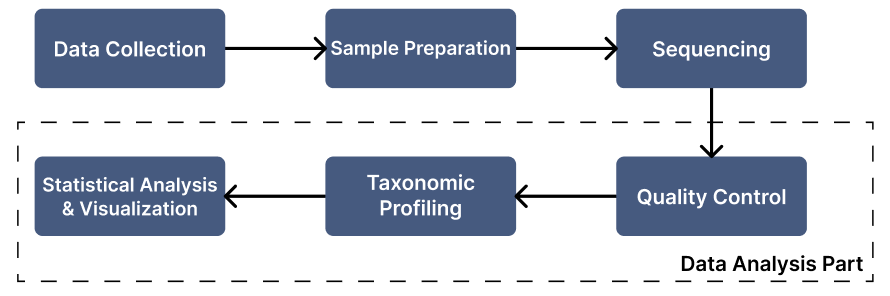
\includegraphics[scale=0.5]{images/state_of_the_art/microbiome_analysis.png}
            \caption{Common microbiome analysis steps}
            \small Microbiome analysis typically follows a structured methodology. The process begins with data collection, followed by sample preparation, sequencing, and ultimately, data analysis. The latter, as depicted by the dashed section in the figure, encompasses steps such as quality control, taxonomic profiling, as well as diversity analysis, and visualization. For methods like shotgun sequencing and metabarcoding, the tools used in the steps above can be different.
            \label{fig:state_of_art:microbiome_analysis}
        \end{figure}

        \paragraph*{Data collection}
        Sample collection is the first step in microbiome analysis and involves collecting samples from the environment of interest, such as soil, water, or host organisms. The use of appropriate sampling techniques is essential to maintain the integrity of the microbial community. Methods such as wiping, filtration, and direct sampling are commonly used and protocols vary depending on the sample type and study objectives.


        \paragraph*{Sample preparation}
        Sample preparation involves a series of procedures to prepare the collected samples for downstream high-throughput sequencing and analysis. Sample preparation encompasses processes that isolate and concentrate microbial DNA or RNA from complex sample matrices, convert it into a format suitable for sequencing, and generate libraries for high-throughput sequencing.

        For metabarcoding, which is also referred to as amplicon sequencing, the sample preparation process involves extracting genomic DNA from the collected samples, amplifying targeted DNA regions using PCR with specific primers (usually 16S rRNA gene for bacteria and ITS region for fungi), and preparing amplicon libraries for sequencing. This targeted approach enables the identification of specific taxa present in the sample, based on the sequenced marker genes. The advantages of this method are its simplicity, speed, low cost, and mature analytical techniques, while the disadvantage is its limitation to the target marker genes so no global genomic functional context.
                    
        In contrast, for shotgun metagenomics, the sample preparation process involves extracting total DNA or RNA from the collected samples, without any targeted amplification. The extracted nucleic acids are then fragmented and converted into sequencing libraries, capturing the entire genetic information within the sample, including both coding and non-coding regions. This approach allows for the characterization of the complete microbial community composition and functional potential within the sample. The limitation of shotgun sequencing is that it is of high cost, often includes contamination including the host, and requires high-performance computing, and high memory.

        \paragraph*{Sequencing}
        
        As for sequencing technologies, there are 2 popular techniques: (1) Illumina and (2) Nanopore. Illumina sequencing is a second-generation sequencing technique that uses reversible dye terminator technology to detect the sequence of DNA molecules. Solexa company, now a part of Illumina company, was founded in 1998. This company invented a sequencing method based on reversible dye terminator technology and engineered polymerases.
                
        In the Illumina sequencing method, the sample is first cleaved into short Fragments. Therefore, in Illumina sequencing, about 100-150bp long reads or fragments are created at the beginning. These fragments are then ligated to generic adaptors and annealed to a slide. Bridge amplification is done to amplify each fragment. This creates a spot with many copies of the same fragment. Later, they are separated into single-stranded fragments and subjected to sequencing. The sequencing slide contains fluorescently labeled nucleotides, DNA polymerase, and a terminator. Because of the terminator, only one base is added at a time. Each cycle terminator has washed away, and it allows the addition of the next base to the site. Furthermore, based on fluorescent signals, the computer detects the base added in each cycle. Illumina sequencing technology constructs the sequence within 4 to 56 hours\cite{quail2008large}.
                
        Nanopore sequencing, a third-generation sequencing method, employs the protein nanopore to determine the nucleic acid sequence of a nucleotide sequence. The technology has seen considerable expansion in both basic and applied research since Oxford Nanopore Technologies (ONT) introduced the first Nanopore sequencer, MinION, in 2014. This technique relies on a nanoscale protein pore, or "nanopore," which serves as a biosensor and is embedded in an electrically resistant polymer membrane \cite{wang2021nanopore}. A motor protein controls the translocation speed by guiding the nucleic acid molecule through the nanopore in a step-by-step fashion. Changes in the ionic current during translocation correspond to the nucleotide sequence in the sensing region, which is then decoded using computational algorithms, allowing for real-time sequencing of individual molecules. Besides regulating translocation speed, the motor protein possesses helicase activity, facilitating the unwinding of double-stranded DNA or RNA-DNA duplexes into single-stranded molecules that can pass through the nanopore.


        \subsubsection{Data analysis}
            As shown in figure \ref{fig:state_of_art:microbiome_analysis}, the data analysis part in the general microbiome analysis contains 3 steps: quality control, taxonomy classification, and diversity analysis and visualization.
            
        \paragraph*{Quality control and pre-processing}
        After sequencing, raw sequence data is subjected to quality control and pre-processing steps by detecting and removing adapter contamination and low-quality reads which could cause reduced accuracy in downstream analysis. Tools such as FastQC \cite{andrews2010fastqc} assess read quality, while Trimmomatic \cite{bolger2014trimmomatic} and Cutadapt \cite{martin2011cutadapt} trim low-quality bases and remove spliced sequences. Pre-processing ensures that only high-quality reads are used for downstream analysis.
        
        \paragraph*{Taxonomic profiling}
        Taxonomic profiling is a crucial step in the microbiome analysis pipeline that aims to identify and classify the microorganisms present in a sample. For metabarcoding (also referred to as amplicon) data, tools such as QIIME2 \cite{bolyen2019qiime2}, Mothur \cite{schloss_introducting_2009} and USEARCH \cite{edgar2010search} assign operational taxonomic units (OTUs) or amplicon sequence variants (ASVs) and assign taxonomy. OTUs are generated through clustering methods. These methods are founded on the principle that organisms with similar target gene sequences are likely to be closely related. In contrast, the ASV approach takes a different route. It begins by identifying the exact sequences that were observed in the sequencing data and quantifying their frequencies. This information is then combined with an error model.
        For shotgun data, classification can be performed using tools such as MetaPhlAn \cite{blanco2023extending} and Kraken \cite{wood2019improved}.


        Below are some state-of-the-art tools and methods used for analyzing metabarcoding data:
        
            \textbf{QIIME 2}
            
                \tool{QIIME 2} represents a cutting-edge, extensible, open-source, and community-developed microbiome bioinformatics platform \cite{bolyen2019qiime2}. 

                QIIME 2 has integrated and automatic data provenance tracking that ensures decentralized tracking of analyses. It eliminates guesswork about the executed commands, as QIIME 2 artifacts, comprising data and metadata, facilitate automatic tracking of data type, format, and provenance. This enhances the replicability and reproducibility of analyses.
                
                Each QIIME 2 artifact is associated with a semantic type that helps identify appropriate inputs for analysis and prevents incompatible artifacts from being used. This semantic type system aids users in avoiding semantically incorrect analyses.
                
                QIIME 2 features a plugin-based system, allowing users to access a broad range of microbiome analysis methods. Users can install plugins developed by both the QIIME 2 team and third-party developers, expanding the availability of tools and techniques.
                
                QIIME 2 supports various user interfaces, including a command line interface (\tool{q2cli}), a web-based graphical user interface (\tool{q2galaxy}), and a Python 3 API (Artifact API). The \tool{q2cli} requires command line interaction but has comprehensive documentation. The \tool{q2galaxy} is user-friendly and requires no command inputs, while the Artifact API is suited for advanced users, supporting interactive computing using Python 3.

                    
            \textbf{Mothur}
            
                \tool{Mothur}, an open-source and extensible microbial community analysis tool, was developed by Schloss et al. at the University of Michigan's Department of Microbiology and Immunology \cite{schloss_introducting_2009}. The tool caters to the bioinformatics analysis needs of microbial community ecology.
                
                \tool{Mothur} integrates algorithms from tools such as \tool{DOTUR}, \tool{SONS}, \tool{TreeClimber}, \tool{LIBSHUFF},  \tool{$\int$-LIBSHUFF}, and \tool{UniFrac}, in addition to its own features.
                
                \tool{Mothur} offers additional features, including diversity assessment, visualization tools like Venn diagrams, heat maps, and dendrograms, sequence quality screening functions, a NAST-based sequence aligner, and a pairwise sequence distance calculator.
                
                Users can run \tool{Mothur} in three modes - interactive, batch, and command line. The interactive mode provides prompt feedback and is ideal for beginners or working with individual files.
                
                \tool{Mothur} has extensive community-supported documentation through a MediaWiki-based wiki and a phpBB-based discussion forum. The wiki format allows users to read, edit, and expand content, promoting diverse experiment design and data analysis.

            \textbf{DADA2}
            
                \tool{DADA2} is a cutting-edge bioinformatics tool designed for fast and accurate sample inference from metabarcoding data with single-nucleotide resolution \cite{callahan2016dada2}. It offers several advantages over traditional methods, making it an essential tool for researchers in the field of microbial ecology and other disciplines that rely on metabarcoding sequencing data.

                \tool{DADA2} is known for its ability to infer exact amplicon sequence variants (ASVs) from amplicon data, resolving biological differences down to 1 or 2 nucleotides. This level of resolution allows for the detection of subtle differences in microbial communities.
                
                \tool{DADA2} is highly accurate in identifying sequence variants, reporting significantly fewer false-positive sequence variants compared to other methods that produce false OTUs. This ensures that researchers can rely on the data generated by \tool{DADA2} for robust downstream analyses.
                
                \tool{DADA2}'s output of ASVs can be directly compared between studies without the need for reprocessing pooled data, facilitating meta-analyses and cross-study comparisons.
                
                \tool{DADA2}'s computational efficiency is another advantage, as the software's compute time scales linearly with the sample number, and memory requirements remain flat. This allows for the analysis of large datasets without compromising on processing time or computing resources.


            \textbf{Comparions of QIIME 2, Mothur and DADA2}

                \begin{table}[H]
                    \centering
                    \begin{tabular}{|l|p{3cm}|p{3cm}|p{3cm}|}
                    \hline
                    \textbf{Feature} & \textbf{QIIME 2} & \textbf{Mothur} & \textbf{DADA2} \\
                    \hline
                    Resolution & High, with the ability to distinguish closely related microbial taxa & High, but inferior to DADA2's single-nucleotide resolution & Single-nucleotide resolution \\
                    \hline
                    Comparability & Extensive interoperability and compatibility with other tools & Limited compatibility with external tools & ASV output allows direct comparisons between studies \\
                    \hline
                    Flexibility & Plugin-based system for expanding microbiome analysis functionality & Allows users to run individual commands, batch files, or directly from the command line & Less flexibility in creating customized analysis pipelines \\
                    \hline
                    User Interface & Offers command line interface, graphical user interface, and Artifact API & Interactive mode, batch mode, and command line mode & Primarily designed for use with the R programming language \\
                    \hline
                    Documentation & Comprehensive documentation and user support & Extensive community-supported documentation & Thorough documentation and community support \\
                    \hline
                    \end{tabular}
                    \caption{Comparison of QIIME 2, Mothur, and DADA2}
                    \label{metabarcoding_tools}
                \end{table}


            Despite the strengths of each of the three tools (QIIME 2, Mothur, and DADA2), QIIME 2 stands out for its versatility, ease of use, flexibility, and community support as shown in the table \ref{metabarcoding_tools}. The plugin-based system and wide variety of user interfaces make it accessible to both novice and experienced users. Moreover, its efficient computational scaling, high accuracy, and interoperability make it an attractive choice for microbial community analysis. The integrated and automatic data provenance tracking feature also greatly enhances the reproducibility and transparency of analyses conducted with QIIME 2, making it a more attractive choice for academic and research settings. While Mothur and DADA2 have their own strengths, they lack the versatility and comprehensive user support that QIIME 2 provides. Therefore, QIIME 2 is considered a superior tool for metabarcoding data analysis in microbial community studies.

            some state-of-the-art tools and methods used to analyze shotgun data are described below:
            
            \textbf{Kraken 2}
            
            \tool{Kraken 2} is a sequence classification system that uses a k-mer based approach to assign taxonomic labels to DNA sequences \cite{wood2019improved}. It is designed to be fast and efficient, making it well-suited for large datasets. \tool{Kraken 2} uses a pre-built database of microbial genomes to classify sequences. \tool{Kraken 2} uses k-mers from the DNA sequences to classify them to the lowest taxonomic rank possible, based on the reference database. The output of \tool{Kraken 2} is a list of taxonomic labels and their relative abundance, which can be used for downstream analysis. \tool{Kraken 2} can also generate reports to help interpret the results.
            
            \textbf{Metaphlan}
            
            \tool{Metaphlan} is a metagenomic profiling tool that uses unique clade-specific marker genes to profile the taxonomic composition of microbial communities \cite{blanco2023extending}. It is designed to be highly accurate and sensitive and can identify both bacteria and archaea. \tool{Metaphlan} includes a pre-built database of marker genes and can generate both abundance and presence/absence profiles. The marker genes used by \tool{Metaphlan} are specific to different taxonomic groups and are used to identify the presence and abundance of those groups in metagenomic datasets. \tool{Metaphlan} 's accuracy and sensitivity make it well-suited for detecting low-abundance microbial taxa that may be missed by other methods. The output of \tool{Metaphlan} includes taxonomic abundance estimates and a taxonomic tree, which can be visualized and used for downstream analysis.
            
            \textbf{mOTUs}
            
            \tool{mOTUs} is a metagenomic clustering tool that groups similar sequences into OTUs based on their genomic content\cite{milanese2019microbial}. It is designed to be highly accurate and specific and can identify both bacteria and archaea. mOTUs includes a pre-built database of microbial genomes and can generate both abundance and presence/absence profiles. \tool{mOTUs} algorithm uses a clustering approach that is based on the pairwise similarity of genomic content between sequences. This approach is useful for providing information on the functional potential of the microbial community. The output of \tool{mOTUs} includes a list of OTUs and their relative abundance, which can be used for downstream analysis.
    
            \textbf{Comparison of Kraken 2, Metaphlan and mOTUs}

            In comparing these tools, \tool{Kraken 2} emerges as the superior option for several reasons. Primarily, \tool{Kraken 2}'s speed and efficiency in handling large datasets make it highly suitable for high-throughput sequencing studies. Its k-mers based approach and comprehensive microbial genome database allow for accurate classification to the lowest taxonomic rank possible. Additionally, the detailed reports generated by \tool{Kraken 2} facilitate the interpretation of results and downstream analysis. While \tool{Metaphlan} and \tool{mOTUs} have their own unique advantages and are both highly accurate and specific, the overall speed, efficiency, and comprehensive reporting offered by \tool{Kraken 2} make it the more desirable choice for shotgun metagenomic analysis.
            

        
        \paragraph*{Diversity analysis and visualization}
        Finally, various diversity analysis methods and visualizations of the analyzed data were performed to determine differences in microbial community structure and function. Alpha diversity and beta diversity are commonly used to measure the diversity within samples and between samples. In addition, specialized software such as Pavian \cite{breitwieser2020pavian} and Krona \cite{ondov2011interactive} provide user-friendly interfaces to generate information visualizations.

    
        By following these general steps above and employing appropriate tools and protocols, researchers can perform comprehensive microbiome analyses to gain valuable insights into the complex microbial communities that underpin various ecosystems and host organisms.


        \subsubsection{Workflow management systems}
            Even with the right analysis tools and methods, the complexity of these studies can often be overwhelming, rendering efficient data management and process automation critical to their successful implementation. Scientists often employ different tools and software at various stages of the analysis, which might not be entirely compatible or require different computational environments to function optimally. Thus, in managing and manipulating the generated datasets, particularly in the context of high-throughput sequencing, we are brought to the doorstep of another fundamental aspect of bioinformatics: Workflow Management Systems.
        
            Workflow management pertains to the process of designing, documenting, monitoring, and refining a sequence of operations required to fulfill a particular task.
        
            In the context of bioinformatics, workflow management systems are pivotal as they streamline and automate multistep computational investigations. They offer a standard lexicon for outlining analysis workflows, which in turn aids in replicability and in the establishment of libraries with reusable components.
            
            The primary advantage of these systems is that they enable bioinformaticians to delegate the reproducibility of workflows and the execution of workflows to the management system. Consequently, researchers can focus their attention on the actual functionality of these workflows, the interpretation of their data, and the advancement of their scientific inquiries.
            
            \paragraph*{Snakemake}
                Snakemake is a workflow management system designed for creating reproducible and scalable data analyses. The system uses a human-readable, Python-based language to describe workflows, enabling seamless scaling to various environments, including servers, clusters, grids, and clouds, without needing to alter the workflow definition. Additionally, Snakemake workflows can include descriptions of necessary software, automatically deploying them to any execution environment\cite{molder2021sustainable}.
                
                Snakemake's core concept involves specifying workflows by decomposing them into rules or steps. Each rule dictates the process of deriving a set of output files from a set of input files, which can be accomplished through a shell command, Python code block, external script (Python, R, or Julia), or a Jupyter notebook. The example Snakemake workflow consists of a workflow definition, a directed acyclic graph (DAG) of jobs representing the automatically derived execution plan, and a script referred to from a rule.
           
                The workflow definition language of Snakemake emphasizes maximum readability, which is vital for transparency and adaptability. Factors influencing readability include the use of known words, intuitive punctuation, and operator usage. 
                
                Snakemake is easily deployable through the Conda package manager, Python package, or Docker container.
          
                During workflow processing, Snakemake tracks input files, output files, parameters, software, and code for each executed job. Upon completion, this information can be accessed through self-contained, interactive, HTML-based reports, facilitating the exploration of results alongside their provenance information. Snakemake reports are portable and archivable, as their presentation does not rely on server backends.
        
                Like many other advanced workflow management systems, Snakemake enables workflow execution to scale across various computational platforms, from single workstations to large compute servers, common cluster middleware, grid computing, and cloud computing. Snakemake's design ensures that scaling a workflow to a specific platform only requires modifying command-line parameters, leaving the workflow itself unchanged. Configuration profiles allow for the persistence and sharing of Snakemake command-line setup for any computing platform.
                
            \paragraph*{Nextflow}
                Nextflow is a platform that facilitates scalable and reproducible scientific workflows using software containers, allowing for the adaptation of pipelines written in widely-used scripting languages \cite{di2017nextflow}. Its fluent domain-specific language (DSL) streamlines the implementation and deployment of intricate parallel and reactive workflows on clouds and clusters, with Linux serving as the foundation for data science.
                
                Nextflow simplifies the process of creating computational pipelines by seamlessly integrating various tasks. It allows for the reuse of existing scripts and tools, eliminating the need to learn a new language or API to begin using the platform.
                
                Nextflow supports Docker and Singularity container technologies, enabling seamless integration with the GitHub code-sharing platform. This feature allows users to create self-contained pipelines, manage versions, and quickly reproduce previous configurations.
                
                Nextflow offers an abstraction layer between the pipeline logic and the execution layer, enabling execution on multiple platforms without modification. Out-of-the-box executors are provided for GridEngine, SLURM, LSF, PBS, Moab, and HTCondor batch schedulers, as well as Kubernetes, Amazon AWS, Google Cloud, and Microsoft Azure platforms.
                
                Built on the dataflow programming model, Nextflow greatly simplifies the development of complex distributed pipelines. Parallelization is implicitly defined by the processes' input and output declarations, resulting in inherently parallel applications that can scale up or out without adapting to a specific platform architecture.
                
                Nextflow automatically tracks all intermediate results generated during pipeline execution. This feature enables users to resume execution from the last successful step, regardless of the reason for stopping.
                
                Nextflow enhances the Unix pipes model with a fluent DSL, simplifying the handling of complex stream interactions. This approach promotes functional composition-based programming, leading to resilient and easily reproducible pipelines.
                
            \paragraph*{Common Workflow Language (CWL)}
                The Common Workflow Language (CWL) constitutes an open standard for outlining the execution of command line tools and their integration to form workflows. CWL-based tools and workflows are compatible with various platforms that adhere to CWL standards, facilitating the scaling of intricate data analysis and machine learning workflows from an individual developer's laptop to massive parallel clusters, cloud, and high-performance computing environments\cite{crusoe2022methods}.
    
                CWL's execution model is explicit, with each tool's runtime environment clearly defined, and any necessary elements specified by the CWL tool-description author. Every tool invocation employs a separate working directory, populated in accordance with the CWL tool description. Additional constructs in the CWL Command Line Tool standard cater to applications requiring specific filenames, directory layouts, and environment variables.
    
                The CWL Workflow Description Standard builds on the CWL Command Line Tool Standard, utilizing the same YAML- or JSON-style syntax and featuring explicit workflow-level inputs, outputs, and documentation. Workflow descriptions consist of a list of steps, including CWL Command Line Tools or CWL sub-workflows, each re-exposing their tool's essential inputs. Inputs for each step are connected by referencing the name of either the common workflow inputs or outputs from other steps. Workflow outputs reveal selected outputs from workflow steps, explicitly indicating which intermediate-step outputs will be returned from the workflow. All connections contain identifiers that CWL document authors are encouraged to name meaningfully.
    
                CWL execution requires the implementation of CWL standards rather than a specific software product. Workflow/tool runners that comply with CWL standards can flexibly execute a user's CWL documents as long as they fulfill the requirements outlined in those documents. However, aspects not defined by CWL standards include Web APIs for workflow execution and real-time monitoring.
    
                The CWL standards impose no technical constraints on file sizes processed or parallel tasks run, with major scalability bottlenecks being hardware-related. As technology advances, CWL standards should keep pace without limiting capabilities.
    
                The CWL ecosystem, developed over the past six years, comprises tools, software libraries, connected specifications, and shared CWL descriptions for popular tools. For example, software development kits (SDKs) for both Python and Java are generated automatically from the CWL schema, enabling programmers to load, modify, and save CWL documents using an object-oriented model corresponding to the standards themselves. Other languages' CWL SDKs can be developed by extending the code generation routines.
    
            \paragraph*{Galaxy}
            
                Galaxy is a versatile open-source bioinformatics platform designed to facilitate the analysis and interpretation of complex biological data. Developed by a collaborative community of researchers, Galaxy is designed to address the challenges faced by life scientists in the era of high-throughput genomics, proteomics, and other histological data\cite{galaxy2022galaxy}.
                By providing a comprehensive set of tools and resources in a user-friendly interface, Galaxy facilitates a collaborative and reproducible approach to biological data analysis, ultimately contributing to the advancement of scientific knowledge.
        
                One of Galaxy's key features is its modular architecture. The architecture allows users to create and share custom workflows that can be customized to address specific biological questions or experimental designs. By integrating numerous analytical tools and resources, Galaxy allows for the seamless processing of data across multiple steps and formats. This supports both novice and experienced researchers in gaining meaningful insights from complex datasets.
        
                The Galaxy web user interface offers a comfortable setting for conducting data analysis. However, its utility can be challenged when it comes to handling repeated or looped tasks. Here, Bioblend, a tool designed to interface with Galaxy's API, becomes invaluable\cite{sloggett2013bioblend}.
        
                An Application Programming Interface (API) is a set of protocols established by a software program, outlining how it can be operated by an external program. Galaxy offers a comprehensive API that facilitates developers in accessing its functionalities through high-level scripts. Notably, the Galaxy user interface is transitioning to be fully based on the Galaxy API.
                
                Currently, there are three methods to interact with the Galaxy API. The first method involves plain HTTP requests, which can be cumbersome. The second method uses an object-oriented package, which, however, is still under development. The third method is using Bioblend. Bioblend is the superior choice for bioinformaticians seeking to automate extensive data analyses from the ground up. This tool enhances collaboration by empowering users to both establish the necessary infrastructure and automate complex analyses over vast datasets within the familiar Galaxy environment.
                
                Utilizing Bioblend offers numerous advantages. It allows for programmatic interaction with the server and offers complex control functionalities like branching and looping, which are currently not achievable in workflows. Moreover, Bioblend helps automate repetitive tasks and promotes integration with external resources.


            \paragraph*{Comparison of workflow management systems}

            Among Snakemake, Nextflow, and CWL, Galaxy emerges as an excellent choice for managing workflows that involve the tools mentioned above for several reasons. This selection is primarily influenced by a few distinguishing attributes of Galaxy.
            
            Firstly, Galaxy is distinguished by its user-friendly interface. In contrast to many other workflow management systems that necessitate advanced technical skills, Galaxy's interface caters to users with varying levels of expertise. The construction of workflows is simplified through intuitive drag-and-drop operations, making it accessible even to novices in the field. Moreover, the visualization capabilities of Galaxy further enhance its usability, enabling clear representation and understanding of the constructed workflows.
            
            Secondly, Galaxy stands out for its robust support system, especially when compared to platforms like Snakemake. While both platforms facilitate various bioinformatics tools, what differentiates Galaxy is its extensive community support. This community backing allows users, including those who may not have advanced expertise, to readily adopt and adapt standardized workflows for their data. For instance, Galaxy integrates widely used tools such as QIIME 2, predominantly for metabarcoding analyses, and Kraken 2 for shotgun data analyses. The seamless integration of these tools within Galaxy's framework simplifies the execution of intricate bioinformatics analyses, thereby promoting efficiency and accuracy in research workflows. Conversely, many alternative systems may necessitate a deeper level of expert knowledge for effective interaction.
            
            Lastly, an integral feature of Galaxy that lends it an edge is the provision of Bioblend, a Python library for Galaxy and BioMart. Bioblend acts as a facilitator for automating extensive data analyses, and simplifying the management of large and complex bioinformatics projects. The integration of a Python-based library within Galaxy's ecosystem offers researchers a powerful tool for scripting and automating data-intensive tasks, enhancing productivity and the reproducibility of analyses.
            
            In summary, Galaxy, with its user-friendly interface, broad tool support, and the ability to automate extensive data analyses via Bioblend, emerges as an excellent choice for managing workflows in bioinformatics. It offers a balanced combination of power, flexibility, and ease of use, making it a reliable and robust choice to be used for workflow implementation.
        
        \subsubsection{Microbiome databases}

           After executing workflows on the data using workflow management systems, microbiome results, and collected data samples can be processed for storage and presentation in a microbiome database. Microbiome databases store microbial community data, metadata, and results of microbial community analyses. These databases are essential to deepening our understanding of microbial ecology, functional dynamics, and their impact on human health and environmental sustainability.
    
            A well-structured microbiome database should contain the following:

            \textbf{Sequence data}
                The database should aggregate and organize various types of sequence data, including 16S rRNA gene sequences, macro-genomic and macro-transcriptomic data. This facilitates comparative analysis and allows researchers to identify taxonomic and functional patterns within microbial communities.
    
            \textbf{Metadata}
                Comprehensive metadata should accompany sequence data detailing relevant information about the sample, such as collection method, location, time, and environmental conditions. This context allows for a deeper understanding of the microbial community and its interactions with the environment.

            \textbf{Accessibility}
                Microbiome databases should ensure accessibility, organization, and standardization of data. This facilitates comparisons between studies and increases the reproducibility and transparency of scientific research.
    
            \textbf{Visualizations}
                Visualizations of the data should be provided. This allows researchers to gain meaningful biological insights more easily instead of just plain text-based results.
    
            \textbf{Collaboration and data sharing}
                Microbiome databases should foster a collaborative research environment by providing mechanisms for data sharing and submission that facilitate the exchange of information and advance scientific knowledge.
            
                In summary, microbiome databases are a valuable resource for bioinformatics research, providing centralized access to a large number of selected microbial data and essential analytical tools. By continuously developing and expanding these databases, researchers can deepen our understanding of the intricate relationships between microbial communities and their environments.

                2 popular microbiome databases are outlined below: (1) Mgnify\cite{richardson2023mgnify} and (2) BacDive\cite{reimer2022bac}.
                
        \paragraph*{Mgnify}
            MGnify is a robust, free-access platform from the European Molecular Biology Laboratory-European Bioinformatics Institute (EMBL-EBI) that facilitates the comprehensive exploration, analysis, and preservation of diverse microbiome datasets. Users can access the data under (\url{https://www.ebi.ac.uk/}). This includes metagenomic, metatranscriptomic, metabarcoding, and assembly data. Essentially, it serves as a hub where researchers submit their data, which MGnify then processes using standardized pipelines for taxonomic and functional analysis\cite{richardson2023mgnify}.

            The platform provides users with the capacity to submit their microbiome studies for analysis, to navigate through a wide variety of analyzed microbiome studies, and to visualize and download the results of these analyses. Furthermore, users can access raw data from the European Nucleotide Archive (ENA). MGnify structures its data according to projects, samples, runs, and analyses, thereby ensuring an orderly and easy-to-navigate resource for microbial genomics research.

            MGnify boosts advanced search and browsing functions, along with a comprehensive API for complex inquiries and data downloads. This enables users to search for particular organisms or proteins with certain functions and to switch seamlessly between projects, samples, and runs. Moreover, MGnify provides a search function within its vast non-redundant database of predicted proteins.

            One key feature of MGnify is its utilization of standardized analysis pipelines and its close cooperation with the European Nucleotide Archive (ENA). This affords a context for interpreting results in relation to other datasets and provides a platform for researchers to analyze their pre-publication data. Additionally, MGnify supports the assembly and reanalysis of any pertinent public dataset from the International Nucleotide Sequence Database Collaboration (INSDC) initiative.

            The team behind MGnify is consistently working to expand and enhance the platform to accommodate the ever-evolving field of microbiome research. Their most recent updates are geared towards simplifying access to MGnify's analyses and derived data products. These include improvements to the website and its associated API, the provision of advanced analysis options directly from the web pages, and a significant revamp of the MGnify protein database.
            
            However, it has its limitations when compared to a dedicated beer microbiome database since MGnify is a general platform for microbiome data. A dedicated beer microbiome database would provide more extensive metadata relating to beer production parameters, such as geographical origin, beer types, and breweries that are interesting for understanding the influence of these factors on the microbiome composition and dynamics.
            
        \paragraph*{BacDive}
            BacDive(\url{https://bacdive.dsmz.de}) - the Bacterial Diversity Metadatabase - is a comprehensive resource providing information linked to bacterial and archaeal biodiversity. The database covers a wide spectrum of data, including taxonomy, morphology, physiology, environment sampling conditions, and molecular biology. As of its 2021 update, BacDive hosts information on 82,892 strains. A majority of the data is manually curated and annotated, ensuring reliable information for researchers\cite{reimer2022bac}.

            A unique feature of BacDive is its user-friendly dashboard(\url{https://bacdive.dsmz.de/dashboard}). This feature, designed to guide newcomers, provides statistical overviews on various aspects of the data, including total strains, species count, average cell size, and optimal environmental conditions. In addition, the dashboard includes an interactive display of 49 graphs across eight categories. Clicking on specific data points initiates a search in the advanced search, the isolation source search, or the TAXplorer, making the dashboard an effective launchpad for data exploration.

            Additionally, BacDive has introduced RESTful web services, offering immediate access to machine-readable data in XML and JSON formats. These services enhance access to BacDive's data and improve linkage to external life science web resources. Moreover, the recent update introduces new data fields and features such as gene name search, plasmid search, and 16S rRNA search.

             Despite its strengths, BacDive does have certain limitations when compared to a dedicated beer microbiome database. Notably, BacDive concentrates solely on bacterial diversity and does not include the fungal microbiome, which is an integral part of the beer microbiome. Additionally, similar to MGnify, BacDive is designed for general bacterial biodiversity and lacks a specific focus on the beer microbiome. Consequently, it may not provide in-depth metadata tailored to beer.

        \subsubsection{Open science}
            Apart from the above necessary steps of microbiome analysis, and different workflow management systems, the analysis in the thesis follows the spirit of Open Science. Since the metabarcoding and metagenomics workflows to analyze the beer microbiome data will be on an open-source platform which will be introduced later. And all the data, code, and deliverables for this thesis will be publicly available on GitHub as well, which welcomes the participation of other enthusiasts. 
            
            It is an innovative movement that seeks to promote the free and accessible dissemination of scientific knowledge and has gained substantial traction in the research community\cite{vicente2018open}. The principles of Open Science, including collaboration, reproducibility, transparency, and accessibility, hold immense potential to transform the landscape of scientific research across various disciplines. Bioinformatics, an interdisciplinary field that combines biology, computer science, mathematics, and statistics to analyze and interpret biological data, is particularly well-suited to benefit from the adoption of Open Science practices.
            
        \paragraph*{Reproducibility}
            Reproducibility, the ability to recreate and validate the findings of a study, is fundamental to the scientific method. In bioinformatics, the reproduction of results often requires access to the original data, computational tools, and detailed documentation of the analyses performed. Open Science promotes reproducibility by advocating for open access to data, software, and protocols, enabling researchers to independently verify and build upon the work of others. Implementing reproducible research practices in bioinformatics not only strengthens the credibility and reliability of scientific findings but also minimizes the duplication effort, and thereby enhances the overall efficiency of the research process.
            
        \paragraph*{Collaboration}
            Collaboration is the cornerstone of scientific progress, allowing researchers from diverse backgrounds to pool their expertise, knowledge, and resources to solve complex problems. In bioinformatics, interdisciplinary collaborations are crucial, as they enable the development of novel algorithms, computational tools, and statistical methodologies that facilitate the analysis of large-scale biological data. Open Science fosters a collaborative environment by encouraging data sharing, cross-disciplinary interactions, and the formation of global research networks. By embracing collaboration, bioinformatics researchers can address the challenges posed by the increasing complexity of biological data and accelerate the discovery of novel insights.
    
        \paragraph*{Transparency}
            Transparency in research encompasses the clear and comprehensive reporting of methodologies, data, and results, ensuring that the scientific process is open to scrutiny and evaluation. Bioinformatics is inherently dependent on complex data and computational analyses, which may inadvertently introduce biases or errors. Open Science emphasizes the importance of transparent reporting, including the provision of raw data, detailed descriptions of analytical pipelines, and the use of open-source software, facilitating critical assessment and enabling further research. Greater transparency in bioinformatics strengthens the validity of research findings and contributes to the development of robust methodologies and best practices.
            
        \paragraph*{Accessibility}
            Accessibility is a key principle of Open Science, promoting the democratization of knowledge by ensuring that research outputs are freely available to all, regardless of geographical location or institutional affiliation. In bioinformatics, access to data, tools, and computational resources is essential for the generation of new knowledge and the advancement of the field. By advocating for open-access publication, data sharing, and the development of open-source software, Open Science endeavors to remove barriers to knowledge dissemination and foster a more inclusive research community. Increased accessibility in bioinformatics empowers researchers from diverse backgrounds and resource settings to contribute to the global body of knowledge, fueling scientific innovation and discovery.
        

    
    
    
    
    
    \subsection{Beer Microbiome}
        Beer, likely the oldest and most widely consumed alcoholic beverage globally, traces its origins back to the Middle East and Egypt \cite{bamforth2000brief}. Historical records reveal detailed accounts of mass production in ancient Babylonian Mesopotamia around 1800 BC \cite{preedy2011beer}.
    
        As a testament to its cultural significance, beer continues to play a pivotal role in daily life across various societies. The brewing process has evolved over time, with innovations and regional variations contributing to the development of diverse beer styles.
    
        Comprising more than 90\% water, beer also contains carbohydrates and alcohol, which, when metabolized in the human body, release a certain amount of energy. The alcoholic content in various beer types varies, typically falling within an estimated range of approximately 3.5 to 10\% weight/volume (w/v) \cite{de2016effects}. In Western societies, malted barley serves as the primary ingredient in beer production, although other grains such as wheat, corn, and rice can also be used. Beer can be broadly classified into two main categories: ales and lagers. While the differences between these categories might appear subtle, they have a crucial impact on the beer's characteristics, including flavor, aroma, and appearance.
                
        Regardless of the specific type, all beers undergo the same essential steps in the brewing process. Each stage plays a vital role in shaping the beer's final profile, allowing brewers to create a wide range of flavors and styles to cater to diverse consumer preferences.

        % \subsubsection{Beer microbiome}

            The beer microbiome is a complex ecological system. It consists of different microbial communities. These communities play a vital role in the production, flavor, and stability of beer. Microorganisms such as bacteria and fungi contribute to the beer fermentation process. In recent years, advanced bioinformatics techniques have helped analyze these microbial communities. This allows scientists to better understand their dynamics and optimize the brewing process.
                    
            \paragraph*{Beer bacterial  microbiome}
                The bacterial component of the beer microbiome includes various \textit{lactic acid bacteria} (LAB) and \textit{acetic acid bacteria} (AAB). These microorganisms produce different organic acids. These acids contribute to the beer's sourness and overall flavor profile \cite{bossaert2021description}. LAB mainly comes from the genera \textit{Lactobacillus} and \textit{Pediococcus}. They produce lactic acid during fermentation. AAB primarily comes from the \textit{Acetobacter} and \textit{Gluconobacter} genera. They are involved in the synthesis of acetic acid. The balance of these bacterial populations is essential. It helps develop desired flavor profiles and maintain product stability.
                
            \paragraph*{Beer fungal microbiome}
                The fungal component of the beer microbiome consists mostly of yeasts. \textit{Saccharomyces cerevisiae} and \textit{Saccharomyces uvarum} are the most prevalent species used in brewing. Yeasts have a crucial role in the fermentation process. They metabolize sugars to produce ethanol and carbon dioxide. This shapes the beer's alcoholic content and carbonation levels. 
                
                Aside from \textit{Saccharomyces}, other types of yeast also play crucial roles. To illustrate, \textit{Kluyveromyces} and \textit{Brettanomyces} species are often detected in lambic and gueuze beers. Notably, \textit{Brettanomyces bruxellensis} has a significant impact by producing the unique aroma that develops during the beer's maturation phase\cite{miguel2022non}.


        \subsubsection{Beer fermentation}
            Conventionally, beer production techniques are classified into two groups: bottom-fermenting (lager-fermenting) and top-fermenting (ale-fermenting) processes. By broadening this classification to encompass mixed fermentations, two additional categories can be integrated: non-spontaneous fermentation and spontaneous fermentation \cite{piraine2021mixed}.
    
            \begin{figure}[h]
                \centering
                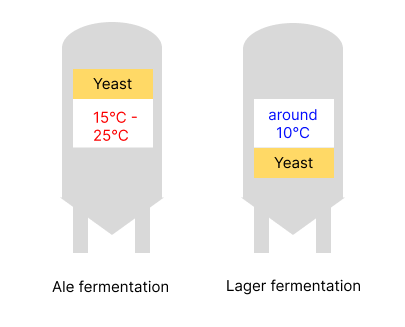
\includegraphics[scale=0.5]{images/beer_fermentation.png}
                \caption{Two types of beer fermentation}
                \small Temperature in Ale (Top) fermentation ideally is between 15°C to 25°C and temperature in Lager (bottom) fermentation ideally is between 6°C and 8°C which is colder compared to Ale fermentation\cite{viejo2019chemical}.
                \label{fig:intro:beer_fermentation}
            \end{figure}
                
            \paragraph*{Top fermentation}
                Top fermentation, also referred to as Ale Fermenting, entails introducing yeast directly onto the wort, where it starts fermenting from the top down. The yeast employed in ale fermentation is \textit{Saccharomyces cerevisiae}, which is also utilized in wine and bread making. 
                
                The ideal fermentation temperature for ale ranges from 15°C to 25°C. Most yeast types perish if the temperature exceeds 40°C \cite{viejo2019chemical}. The yeast used in lager fermentation can tolerate higher alcohol concentrations, which is why top-fermented beers generally have higher alcohol content than bottom-fermented beers. This yeast accelerates the fermentation process, allowing ale to be ready for consumption within a week. In general, top-fermented beers exhibit more robust flavors.

            \paragraph*{Bottom fermentation}
                In bottom fermentation or Lager Fermenting, the yeast in the wort starts working from the bottom up. The yeast typically employed for lager fermentation is \textit{Saccharomyces uvarum}. The optimal temperature range for lager fermentation lies between 6°C and 8°C \cite{viejo2019chemical}.

                Lager yeast becomes inactive when alcohol content surpasses a certain threshold, resulting in lager generally having a lower alcohol content than ale. The fermentation process is considerably slower than that of top fermentation beers, yielding a clearer and more refreshing beer.
                
            \paragraph*{Spontaneous fermentation}
                Spontaneous fermentation is an ancient and natural method of beer production, harnessing the power of wild, ambient microorganisms, predominantly yeast, and lactic acid bacteria, to convert the fermentable sugars in the wort into alcohol, carbon dioxide, and various flavor compounds. This uncontrolled and serendipitous process relies on the unique microbial ecosystem of a given environment, imparting distinctive, complex, and often unpredictable flavors to the resulting beer. The most notable example of spontaneously fermented beer is the Belgian Lambic, a sour and wild-fermented ale that reflects the rich microbiota of the Senne River Valley\cite{spitaels2014microbial}. Spontaneous fermentation is revered for its ability to capture the essence of a specific terroir and its innate capacity to produce unparalleled flavor profiles. However, due to the uncontrollable nature of wild microorganisms, the process can yield inconsistent results and may require lengthy maturation periods.

                While wild yeast, lactic acid bacteria (LAB), and certain other bacteria are typically deemed contaminants in many beer fermentation procedures, these same microorganisms are often desired in the crafting of specific sour beers and wild beer styles. Currently, the international beer market is witnessing a renewed interest in sour beers, as breweries of various sizes globally are exploring new product varieties and complex flavors\cite{bossaert2021description}. For instance, American Coolship Ales, a beer undergoing a complex series of spontaneous fermentations, is gaining popularity for its distinctive flavor profile\cite{bokulich2012brewhouse}. 
                
                This trend underscores the role of these traditionally "undesirable" microorganisms in creating novel and intriguing brews. More and more interest has been focused on identifying these microorganisms.
                
            \paragraph*{Non-spontaneous fermentation}
                In contrast, non-spontaneous fermentation is a controlled and deliberate process that employs selected strains of yeast and, occasionally, bacteria to ferment the wort. This method allows brewers to manipulate various parameters such as fermentation temperature, yeast strain, and wort composition, thereby enabling the production of a vast array of beer styles with consistent and reproducible characteristics. Non-spontaneous fermentation is the predominant method used in modern brewing, given its capacity for precision and the ability to tailor specific flavor profiles to cater to consumer preferences. Examples of beers produced through non-spontaneous fermentation include lagers, and ales, each showcasing distinct flavors and attributes attributed to the particular yeast strains employed and the conditions under which fermentation occurs\cite{white2010yeast}.
    
    
        \subsubsection{Beer microbiome studies overview}
            In this thesis, we have picked five studies related to beer microbiome analysis. Investigating these previous studies is beneficial for our beer microbiome analysis because it allows us to identify and understand the microbial compositions documented in earlier research and we can identify common trends and patterns. By reproducing the results using the data from the studies and comparing them with the original results, we can have a better understanding of our workflows' capability and performance. Among these, we have chosen to focus in detail on three studies that exhibited a higher variety of beers analyzed and were also among the most recent. They are BeerDeCoded: the open beer metagenome project\cite{sobel2017beerdecoded}, Bacterial and Fungal Dynamics During the Fermentation Process of Sesotho, a Traditional Beer of Southern Africa\cite{cason2020bacterial}, Characteristics of bacterial and yeast microbiomes in spontaneous and mixed-fermentation beer and cider \cite{tyakht2021characteristics}, A Culture-Independent Comparison of Microbial Communities of Two Maturating Craft Beers Styles\cite{costa2022culture} and Description of the temporal dynamics in microbial community composition and beer chemistry in sour beer production via barrel aging of finished beers \cite{bossaert2021description}. 3 of the 5 studies mentioned had a higher variety of beers, so they are discussed in detail here.
            
            \paragraph*{BeerDeCoded: the open beer metagenome project}
                The BeerDeCoded project analyzed the targeted metagenomic profile of 39 bottled beers using ITS sequencing of fungal species. These 39 commercial beers originated from 5 different European countries: 30 were from Switzerland, five from Belgium, two from Italy, one from France, and one from Austria.

                After extraction and sequencing the ITSs, a refined set of ITS sequences from the RefSeq database\cite{o2016reference} (Targeted Loci) was utilized to construct an ITS index for the \tool{Burrows-Wheeler Aligner (BWA)} \cite{li2009fast}. Using standard parameters, the \tool{BWA} was applied to align the beer sample reads, which are stored in \tool{FASTQ} format to this ITS index. Subsequently, the files were sorted and indexed using \tool{samtools} \cite{danecek2021twelve}. These BAM files underwent a quality control assessment with the aid of \tool{SAMstat}\cite{lassmann2011samstat}. To ensure accuracy and to remove low-quality, non-uniquely mapped reads, a minimum mapping quality (MAPQ) score of 3 was set as the threshold. Following this, the count of ITS per beer and per species was calculated, with only species having more than 10 reads considered for further analysis.
                
                The analysis revealed 42 distinct fungal species, intriguingly, 24 of these species were exclusive to just one type of beer. The extensive diversity of wild yeasts present in commercial beers was unanticipated, with some beers exhibiting evidence of containing over 10 different fungal species.
                
                Waldbier 2014 Schwarzkiefer, an Austrian beer incorporating pine cones sourced from local forests in its brewing process, stood out with the highest internal transcribed spacer (ITS) diversity, comprising 19 fungal species. In addition, two other beers both showed over 12 fungal species: La Nébuleuse Cumbres Rijkrallpa, a sour/wild ale that incorporates cranberries and fermented corn known as "Chicha", and Chimay Red Cap, a traditional Belgian Trappist beer.
                
            \paragraph*{Bacterial and Fungal Dynamics During the Fermentation Process of Sesotho, a Traditional Beer of Southern Africa}
                Sesotho, a widely consumed spontaneously fermented beer in Lesotho, Southern Africa, is brewed from milled maize, sorghum, or wheat flour, sometimes a blend of these. This beer is recognized for its cloudy appearance, light body, and characteristic sour taste. The goal of this study was to scrutinize the microbial diversity, covering both bacterial and fungal species, across five distinct stages of Sesotho fermentation. This was done at five unique locations in Lesotho, using Next-Generation Sequencing (NGS) methodologies.
                
                Ensuring data integrity and precision, all data sets underwent initial processing and trimming, with the aim of achieving an average quality score of at least 20. Sequences shorter than 200 base pairs were excluded. Subsequently, paired-end reads were amalgamated. A demultiplexing and quality filtering script in \tool{QIIME} was executed with default parameters, producing a FASTA output file. Chimeric sequences, or abnormal sequences composed of two distinct sequences, were recognized and removed. Then representative Operational Taxonomic Units (OTUs) were taxonomically classified, adhering to a 97\% sequence identity standard against the SILVA 132 database for the 16S rRNA bacterial data, and the UNITE database for the fungal ITS data.
                
                For the bacterial results, 9,885 bacterial OTUs were identified, with individual samples containing between 600 and 2,543 OTUs. \textit{Proteobacteria} and \textit{Firmicutes} emerged as the dominant bacterial phyla across all samples and locations. Regarding fungi, 46 OTUs were detected at the same sequencing depth across all samples, with individual samples yielding between 5 and 13 OTUs. The prevailing fungal phyla across all samples and locations were \textit{Ascomycota} and \textit{Mucoromycota}, with \textit{Saccharomyces spp}. being an example of the Ascomycota. This research offers valuable insights into the microbial ecology involved in Sesotho beer fermentation.
                
            \paragraph*{Characteristics of bacterial and yeast microbiomes in spontaneous and mixed-fermentation beer and cider}
                This study concentrates on the microbial communities within 14 commercially available Russian beers, known for their mixed or spontaneous fermentation. These beer samples were either acquired from retail stores or directly supplied by the manufacturers. The analysis hinged on High Throughput Sequencing of 16S rRNA and ITS regions from these beer samples.

                The data was processed utilizing the \tool{Knomics-Biota system}, which was enhanced by authors to scrutinize the prokaryotic and yeast microbiomes associated with food products. Firstly, the reference databases were expanded to accommodate 16S rRNA sequencing data from any niche. Secondly, a new module was incorporated for analyzing the fungal ITS region. This module is based on the UNITE database \cite{nilsson2019unite}, utilizes the Deblur algorithm \cite{amir2017deblur} for amplicon-sequence variant (ASV) identification, and employs the \tool{QIIME2 naive-Bayes classifier}.
                
                Given the diversity in the samples, which encompassed mixed-fermentation beer, it was anticipated that the yeast composition would not be restricted to \textit{Saccharomyces cerevisiae}. As hypothesized, the microbiome was primarily influenced by the balance between \textit{Dekkera} (also known as \textit{Brettanomyces}) and \textit{Saccharomyces}, while other less prevalent contributors included \textit{Issatchenkia}, \textit{Pichia}, \textit{Hanseniaspora}, and \textit{Candida}. On a species level, \textit{Dekkera} was predominantly represented by \textit{D. bruxellensis}, with minor presence of \textit{D. custersiana} and \textit{D. anomala}. \textit{Saccharomyces} was chiefly represented by \textit{S. cerevisiae} and \textit{S. bayanus/pastorianus} among others. On the other hand, the bacterial community was predominantly composed of members from the \textit{Lactobacillales} order. Other bacterial families were generally found in low abundances in the beer samples, except for three instances where the \textit{Enterobacteriaceae}, \textit{Leuconostocaceae}, and \textit{Acetobacteraceae} families were present in considerable (>5\%) quantities.

            \paragraph*{Summary of prior beer microbiome studies}
                These 3 studies focus on different types of beer, but all studies employ metagenomic profiling, targeting fungal ITS and bacterial 16S rRNA regions, to investigate the microbial communities in beers. And the studies utilize similar data analysis steps just like discussed previously, such as quality control, taxonomic profiling, and diversity analysis \& visualization. Across the studies, the predominant fungal phylum observed is \textit{Ascomycota}, within which \textit{Saccharomyces spp}. are identified as key contributors to the beer microbiome. This genus is known for its pivotal role in the fermentation process. The studies report \textit{Proteobacteria} and \textit{Firmicutes} as dominant bacterial phyla, with members of the \textit{Lactobacillales} order frequently detected. These bacteria are responsible for the production of lactic acid and other metabolites that impact beer flavor profiles.
                
\section{Methods}

    This section provides a comprehensive overview of the methodologies employed in various stages of our research. These stages are i) collection of beer microbiome data samples; ii) implementation, evaluation, and automation of bioinformatics analysis workflows for the data and reproducibility analysis; and iii) the construction of the beer microbiome database, BeerMicroDB, which was designed to serve as a comprehensive overview of beer microbiome data and the reproduced results using the workflows created. 
    
    \subsection{Data collection}

        In the beginning, due to uncertainty about the adequacy of beer-related data samples, the decision was made to collect samples not only of beer but also of cider, Kombucha, kefir, and wine. The procedure for data collection was bifurcated. The first avenue involved seeking out research articles on the microbiome of fermented drinks via Google Scholar. The availability of public sample data was then verified for each paper. If such data was available, it was added to a spreadsheet along with relevant metadata. The second method involved a direct search for microbiome samples related to fermented drinks in databases such as ENA or MG-RAST \cite{keegan2016mg}. Any suitable datasets found this way were also added to the spreadsheet. In total, 768 samples were collected.
        
        Once data collection was completed, the Python libraries \tool{pandas} and \tool{matplotlib} were used in a \tool{Jupyter Notebook} to graphically represent the data, facilitating a preliminary understanding of its composition.

        \begin{figure}[H]
            \centering
            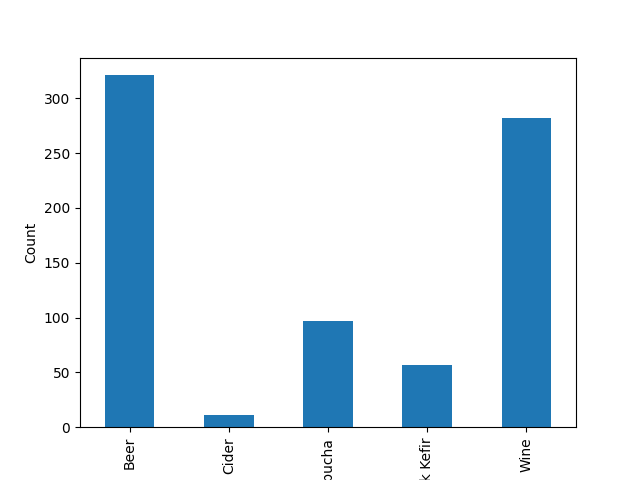
\includegraphics[scale=0.5]{images/methods/data_composition_by_type.png}
            \caption{Overview of fermented drinks}
            \label{fig:methods:data_composition_by_type}
            \small Number of data samples by fermented drink types, which consist of Beer, Cider, Kombucha, Milk Kafir, and Wine.
        \end{figure}

        To deepen our understanding of the collected data, we first examine the number of samples associated with each type of fermented drink shown in figure \ref{fig:methods:data_composition_by_type}. Subsequently, to enhance our insight, we explore how these samples are distributed across various extraction techniques, such as shotgun and metabarcoding techniques. For the metabarcoding approach, we pay special attention to the distribution of sequencing targets, including but not limited to ITS and 16S shown in figure \ref{fig:metabarcoding_data}.

        \begin{figure}[H]
             \centering
             \begin{subfigure}[b]{0.45\textwidth}
                \centering
                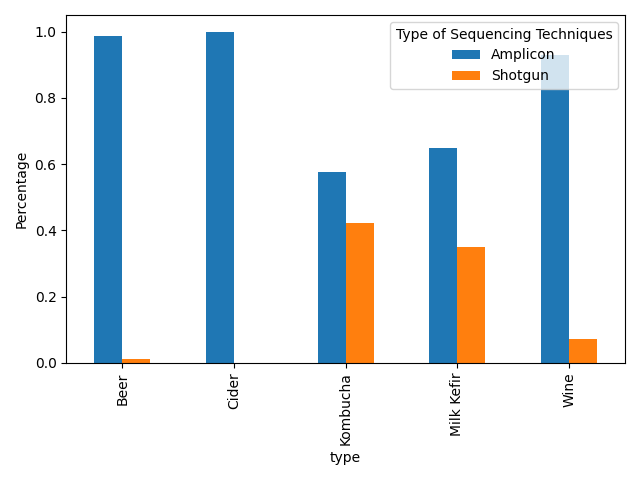
\includegraphics[scale=0.5]{images/methods/data_composition_by_sequencing_techniques.png}
                \caption{Data composition by sequencing techniques}
                \label{fig:methods:data_composition_by_sequencing_techniques}
             \end{subfigure}
             \hfill
             \begin{subfigure}[b]{0.45\textwidth}
                \centering
                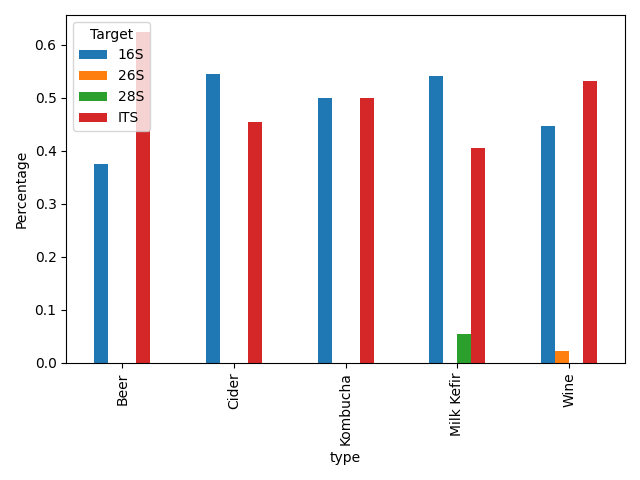
\includegraphics[scale=0.5]{images/methods/metabarcoding_data_composition_by_targets.png}
                \caption{Metabarcoding data composition by targets}
                \label{fig:methods:metabarcoding_data_composition_by_targets}
             \end{subfigure}
                \caption{Data composition by sequencing techniques and metabarcoding targets}
                \label{fig:metabarcoding_data}
        \end{figure}

        Through meticulous data collection, we have assembled a substantial array of beer samples. Our observation indicates that the majority (higher than 95\%) of our metabarcoding data  can be categorized as either ITS or 16S.  The beer sample did not even have 26S and 28S data. With this in mind, and given the adequate amount of data for the beer samples, which is over 300, we have chosen to focus only on these beer samples at the moment.

        While we're concentrating on beer samples now, we're open to the prospect of incorporating data on other fermented drink types in the future. Our current database comprises 317 beer samples. We found that a small subset of these samples (16 to be precise) are housed on the MG-RAST platform, in the form of FASTA files, while all other data samples are in the form of FASTQ files, for keeping consistency, we decided to omit these from our immediate analysis.
        
        In conclusion, our study will concentrate on the remaining 301 beer samples. The volume of data contained within these samples establishes a robust foundation for our continuing investigations. We have made the scripts for plotting the figures, as well as information about the datasets, accessible to the public. These resources can be accessed at the following URL: \url{https://github.com/asdsd/sdfdfs/blob/main/data_plot_n_processing/data_plot.ipynb}.

    
    \subsection{Microbiome analysis workflows}

        This section shows the implementation and evaluation of the workflows used in the thesis and also the methodologies and tools used in the reproducibility analysis.
        
        \subsubsection{Implementation of workflows}

        This section illustrates the implementation of metabarcoding and shotgun workflows accordingly.
        
        \subsubsection*{Metabarcoding workflow}
            Based on the characteristics and comparison of state-of-the-art tools for analyzing metabarcoding data discussed in the section "State of the art: Data Analysis" we use QIIME 2 as the workflow for analyzing metabarcoding data.

        \paragraph*{QIIME 2 Set up on Galaxy Europe}
            QIIME 2 was available as 109 Galaxy wrappers and initially not available on Galaxy Europe and therefore needed to be installed. This involved extracting the QIIME 2 Galaxy tools from the qiime2/galaxy-tools GitHub repository, which contains Official QIIME 2 tools for Galaxy, by using scripts designed to extract all tool IDs into a YAML file and subsequently merging them into the usegalaxy-eu/usegalaxy-eu-tools repository.
        
        After completing this process, the QIIME 2 tools can be accessed through the Galaxy Europe instance. However, to ensure that these tools are executed using docker when invoked, the associated tool IDs must also be added to the job\_conf.yml file in the usegalaxy-eu/infrastructure-playbook repository.
        
        Thus, with the above procedure, the QIIME 2 tools have been successfully configured on the Galaxy Europe instance. The scripts for setting up QIIME 2 on Galaxy Europe can be accessed at the following URL: \url{https://github.com/YedilSerzhan/beer_microbiome/tree/main/qiime2_tools_crawler}.

        \begin{figure}[H]
            \centering
            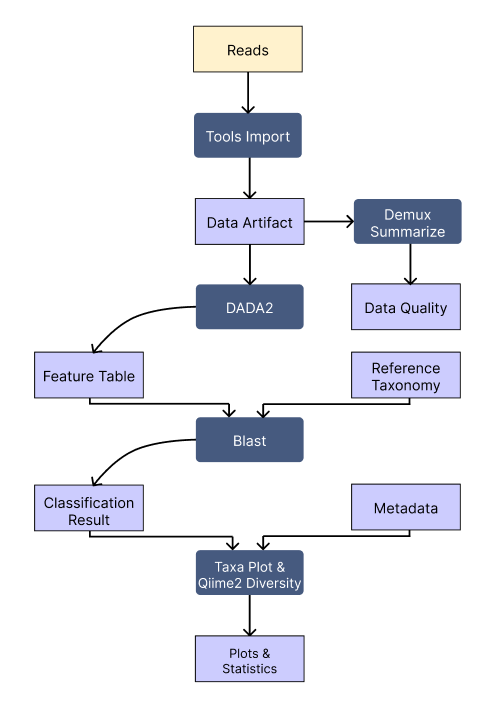
\includegraphics[scale=0.5]{images/metabarcoding_workflow.png}
            \caption{The metabarcoding workflow}
            \small The metabarcoding workflow is implemented using QIIME 2. The steps contain data importing, DADA 2 denoising, taxonomy profiling using BLAST, and visualization \& diversity analysis. (Elements with dark blue color are for tools and purple color are for results of the intermediate steps)
            \label{fig:methods:amplicon_workflow}
        \end{figure}
            
        \paragraph*{Data importing}
            Firstly data files from ENA should be uploaded to Galaxy using the upload function. However, all QIIME 2 tools interact with artifacts instead of traditional data files like FASTQ or FASTA files. A QIIME 2 artifact is a file with .qza extension. In order to convert the input data to an artifact, the tool \tool{qiime2 tools import} needs to be used. There is one parameter "Type of data to import" that needs to be set. For a FASTQ data file, we should choose the "SampleData[PairedEndSequencesWithQuality]" option. Then we need to specify the data file and the file format to import from. Normally in the QIIME 2 CLI version, we can choose the files and format by creating a manifest file, which declares the name and location of each data file to be imported. However, in Galaxy, the location of uploaded data files can't be accessed for security reasons. So in QIIME 2 Galaxy version, we can do it by choosing the option "Casava One Eight Single Lane Per Sample Directory Format" and renaming each data file to the format like "L2S357\_15\_L001\_R1\_001.fastq.gz".The underscore-separated fields in this file name are (1) the sample identifier (2) the barcode sequence or a barcode identifier (3) the lane number (4) the direction of the read (i.e. only R1, because these are single-end reads) and (5) the set number. This certainly has set some limitations for the variety of types of data to process, for example, FASTA files can not be properly processed using QIIME 2 Galaxy.


        \paragraph*{Quality control and feature table construction}

            After importing the data, the quality of the data can be accessed using the tool \tool{qiime2 demux summarize}, which can provide an interactive plot of the quality of the data. Next depending on the data quality information, parts of the data can be truncated or trimmed. 

            The quality control and amplicon sequence variant (ASV) feature table construction can be done using the tools \tool{DADA2}. Deblue is also available for feature table construction but it needs additional quality filtering steps, so dada2 is chosen here. Rather than adopting the conventional approach of "OTU-picking" that is commonly used in metabarcoding workflows, DADA2 \cite{callahan2016dada2} introduces a unique algorithm that simulates the inaccuracies generated in the course of metabarcoding. By employing this error model, the algorithm can deduce the actual composition of a sample. It generates tables of amplicon sequence variants (ASVs), which provide a higher level of resolution in comparison to traditional methods. Based on whether the data is paired or not,  \tool{qiime2 dada2 denoise-single} or \tool{qiime2 dada2 denoise-paired} will be used.
            
            \textbf{Options:}
                For DADA2 denoising, depending on the quality of the data, a few parameters can be set: 1. "trunc\_len": Position at which sequences should be truncated due to a decrease in quality. 2."trim\_left": Position at which sequences should be trimmed due to low quality  3. "max\_ee": Reads with a number of expected errors higher than this value will be discarded. This procedure takes normally around 10 minutes depending on the size of the data. These options should be set depending on the quality information gotten from the result of \tool{qiime2 demux summarize}. 
            
            \textbf{Outputs:}
                The outputs consist of 3 files. 1. "feature table": The resulting feature table is a tabular representation of the data that maps samples to ASVs.  2. "representative sequences": The resulting feature sequences. Each feature in the feature table will be represented by exactly one sequence. 3. "denoising stats": stats about the denoising procedure like how many reads are removed, the percentage of reads that are preserved, and so on. This information can help you have an understanding of how well the denoising is conducted and whether you want to change the parameters and do it again.
    
            \textbf{Visualization for outputs:}
                In order to view the output results, we can use the following tools. For a feature table, we can use \tool{qiime2 feature-table summarize} to generate visual and tabular summaries of a feature table. For the denoising stats, we can use \tool{qiime2 metadata tabulate} to generate a visualization that shows a tabular view of data. And it supports interactive filtering, sorting, and exporting to common file formats.


        \paragraph*{Taxonomy profiling}
            In this step, we’ll perform annotation of the features that were observed in the last denoising step by performing taxonomic classification of the sequences. The tool used in the workflow is \tool{qiime2 feature-classifier classify-consensus-blast}, the function of which is assigning taxonomy to query sequences using BLAST+. Performs BLAST+ local alignment between query and reference reads, then assigns consensus taxonomy to each query sequence from among max accepts hits, min consensus of which share that taxonomic assignment.
    
            \textbf{Inputs and reference database:}
            The required inputs for this tool are  1. Query sequences. 2. Reference sequences. and 3. reference taxonomy labels. The query sequences come from the output representative sequences of DADA 2 denoising. The reference sequences and reference taxonomy labels come from a reference database that we can choose. Until now, for QIIME 2, the available options are UNITE for fungal ITS, Silva for 16S/18S rRNA, and Greengenes for 16S rRNA. In our case, we stick to UNITE for fungal ITS and Silva for 16S rRNA.  

            \textbf{Optional parameters:}
            There are 4 important optional parameters that can be set for consensus-blast. (1) maxaccepts: the maximum number of hits to keep for each query. The first N hits will be chosen in the reference database that is similar to the query the default value is 10. (2) perc\_identity: A float number from 0.0 to 1.0 to reject a match if the percent identity to query is lower. The default value is 0.8. (3) query-cov: A float number from 0.0 to 1.0 with a default value of 0.8. The algorithm rejects matches if query alignment coverage per high-scoring pair is lower than this value. (4) min-consensus: A float number ranging from 0.5 to 1.0 represents the minimum fraction of assignments that must match the top hit to be accepted as consensus assignments. The default value is 0.51. Throughout the processing of all data, most of them are set to use the default values.

            \textbf{Algorithm outputs:}
            There are 2 outputs generated in the end. They are classification and search results. The classification file is the taxonomy classifications of query sequences. And the search results file shows the top hits for each query.

                Both files can be visualized using the \tool{qiime2 feature-table summarize} tool.


        \paragraph*{Diversity analysis and visualization}
            For a more comprehensive grasp of the results, we can employ diversity analysis to assess the richness and diversity within and among the samples. The use of visualization tools can further enhance our insight into the results, offering a more detailed and intuitive understanding of the data.

            There are 2 tools that can be used to do the diversity analysis. The tool \tool{qiime2 diversity alpha} is for computing a user-specified alpha diversity metric for all samples in a feature table. And tool \tool{qiime2 diversity beta} can be used to compute a user-specified beta diversity metric for all pairs of samples in a feature table. The input is the feature table generated by the dada2-denoising tool. And we can choose a metric out of dozens of options.

            Apart from visualizing the intermediate results from the previous steps using tools \tool{qiime2 metadata tabulate} and \tool{qiime2 feature-table summarize}. We can also use \tool{qiime2 taxa barplot} to generate an interactive bar chart visualizing the taxonomic classification results. 

                The inputs are (1) Feature table: the feature table generated by the DADA2 denoising tool. And (2) Taxonomy: Taxonomic annotations for features in the provided feature table, which is the file generated by the tool \tool{qiime2 feature-classifier classify-consensus-blast}.

                The output file is a barplot.qzv file which can be visualized using the QIIME 2 View website to generate an interactive bar chart plot can include multi-level sorting from level 1 kingdom to level 7 species, plot recoloring, sample relabeling, and SVG figure export. If a proper metadata file is also provided as input, you can also group and sort by the metadata columns. 

        
        \subsubsection*{Shotgun workflow}
        
            As we transition to the more comprehensive shotgun sequencing approach, which indiscriminately sequences all the DNA within a sample, we are met with a change in both the scope and the complexity of the analysis. Consequently, the workflow for shotgun sequencing requires a shift in the analytical tools and methods employed. This section talks about the workflow implementation for shotgun data.
            
        \paragraph*{Existing workflow}

            There is already a Galaxy tutorial available on workflows on identifying beer micro-organisms before this thesis (\url{https://training.galaxyproject.org/training-material/topics/metagenomics/tutorials/beer-data-analysis/tutorial.html}).
                        
            \begin{figure}[H]
                \centering
                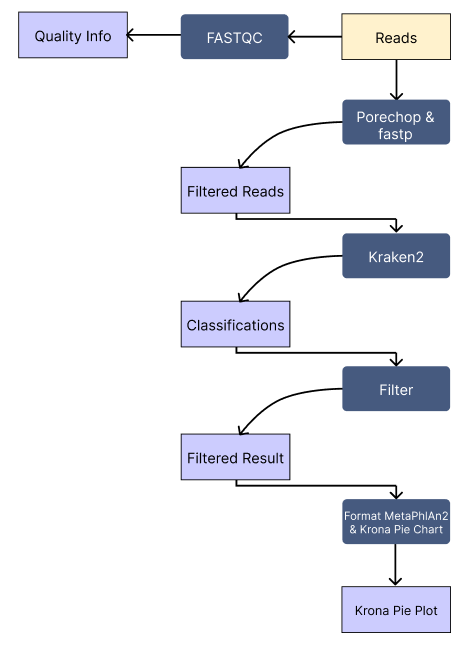
\includegraphics[scale=0.5]{images/existing_shotgun_workflow.png}
                \caption{The existing shotgun workflow}
                \small The existing workflow initiates with quality control measures employing tools such as FASTQC, Oirechop, and fastp. Subsequently, taxonomic profiling is undertaken using Kraken 2. Once profiled, the filtered results are visualized utilizing the Format MetaPhAn2 and Krona Pie charts.
                \label{fig:methods:existing_shotgun_workflow}
            \end{figure}

            The established workflow illustrated in figure \ref{fig:methods:existing_shotgun_workflow} begins with the utilization of \tool{FASTQC} \cite{andrews2010fastqc} to evaluate the quality of the reads. The resulting HTML file vividly portrays the quality scores distributed over all bases. \tool{Porechop} \cite{wick2017completing} is subsequently employed to eliminate sequencing adapters and chimeras, or contaminants. Moreover, the tool \tool{fastp} \cite{chen2018fastp} aids in filtering sequences possessing low-quality scores. One can review the HTML report generated by \tool{fastp} to ascertain how the data quality has been enhanced.

            The subsequent step is taxonomic classification, for which we utilize \tool{Kraken2}. The database incorporated in this phase is the "Prebuilt Refseq indexes: PlusPF". If the "Create Report" option in Kraken2 is selected, a report file encompassing detailed information is produced. The report's first column displays clades, extending from taxonomic domains (like Bacteria, Archaea, and so forth) to species. The second column discloses the number of reads allocated to the clade rooted at that particular taxon.
            
            For visualizing the results, we employ \tool{MetaPhlAn2}  \cite{blanco2023extending} to transfigure the report into the Krona format. Subsequently, the \tool{Krona pie chart} tool can process the converted report file to construct a Krona pie chart. This chart is a multilayered pie chart that exhibits the community profile. The central part of the chart represents higher taxonomy levels (such as the domain), whereas the outer parts provide more detailed information (such as species).
            
        \paragraph*{Updates to the shotgun workflow}

            The existing workflow for shotgun sequencing analysis has been in place for an extended period. During this time, there have been significant updates to both the tools and databases involved in the process. Notably, the advent of the Kraken software suite \cite{lu2022metagenome} has necessitated further updates to the shotgun workflow.

            \begin{figure}[H]
                \centering
                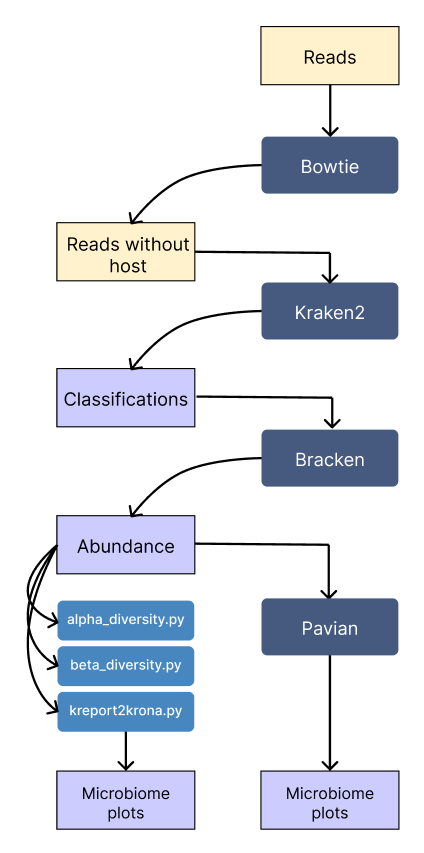
\includegraphics[scale=0.5]{images/shotgun_workflow.png}
                \caption{The shotgun workflow}
                \small Relative to the previous workflow, the updated procedure incorporates Bowtie2 at the outset to eliminate host DNA from the reads. Following the classification by Kraken 2, the data is processed by Bracken to yield abundance information. This information is subsequently visualized using Pavian and KrakenTools, as depicted by the three scripts presented in the figure.
                \label{fig:methods:new_shotgun_workflow}
            \end{figure}
            
        The process of the shotgun workflow illustrated in figure \ref{fig:methods:new_shotgun_workflow} commences with the removal of human host DNA using Bowtie2. For some datasets collected, the host DNA is already removed, then this step can be skipped.

        Then it is followed by the taxonomic classification of sequencing reads using \tool{Kraken2}\cite{wood2019improved}. Each read is then allocated to a taxonomic group (species, genus, or higher-level taxa). The database used here is Standard plusPFP (Standard plus protozoa, fungi, and plant) version 2022-06-07. Optionally a report can be generated showing the aggregate counts of each classified result.
        
        And then subsequent step involves calculating the relative abundance of different species within the sample. \tool{Bracken} was devised to function alongside \tool{Kraken 2} for species abundance computation, utilizing the classification results from \tool{Kraken 2}. \tool{Bracken} \cite{lu2017bracken} then processes the classified read counts and estimates the abundance of each taxon in the sample.
        
        In the final analysis, \tool{KrakenTools} and \tool{Pavian} \cite{breitwieser2020pavian} offer a comprehensive toolkit for downstream statistical analysis and visualization of the classification and abundance estimation outcomes.
        
        \tool{Pavian} can be employed to examine and visualize the sample to identify differences. In addition, \tool{alpha\_diversity.py} can be utilized to measure the diversity in a sample, and \tool{beta\_diversity.py} can be applied to compare diversity across samples. \tool{kreport2krona.py} can convert the Kraken report into the Krona format, which can be visualized using \tool{Krona} by generating a Krona plot.

          \tool{KrakenTools} are not available in the suite of Galaxy tools, hence there is a need to integrate them into the Galaxy EU instance. The process of doing so involves several steps:

            1. Construct the Wrappers
            
            \tool{Planemo} is a command-line utility employed in creating Galaxy and Common Workflow Language artifacts, which encompass tools, workflows, and training materials. The procedure commences with the command planemo tool\_init --id 'id' --name 'name', which generates an XML file containing significant tags such as requirements, command, inputs, outputs, and help.
            
            The requirements tag should include the necessary packages to execute the tool that requires wrapping. For \tool{KrakenTools}, this mainly pertains to Python.
            
            The command tag houses the command line necessary to operate the tool, comprising input files, parameters, and outputs. These options will subsequently be defined in the inputs and outputs sections.
            
            The inputs tag encompasses the tool's input, which will be displayed on the tool's page within Galaxy for users to select input files or parameters. The input encompasses several parameter types, including data, integer, float, and boolean values. Advanced tools may also permit the setting of conditional parameters.
            
            The outputs tag involves the tool's output, which should also be encompassed within the commands.
            
            The help tag should offer valuable information to assist new users in learning how to employ the tool.

            Proper configuration is essential for creating a user-friendly interface that facilitates easy understanding of the tool. This consideration is not only vital for the current workflow but also for all researchers utilizing the Galaxy platform.
            
            2. Construct Test Cases
            
            A proficient tool wrapper should include tests to ensure the smooth operation of the tool. These tests can also be set within the XML file. Multiple tests can be constructed, each involving example inputs and example outputs. 
            
            \tool{Planemo} utilizes the commands in the XML file to generate results using the inputs. If the generated result aligns with the anticipated outputs, it is declared that the tool is functioning correctly. All potential edge cases should be taken into account in these tests. Importantly, the example input and output files should not exceed 1MB in size.
            
            3. Submit the Pull Request on Tools-IUC
            
            Tools-IUC (https://github.com/galaxyproject/tools-iuc) is a GitHub repository that contains a selection of Galaxy repositories used in the Tool Shed (https://toolshed.g2.bx.psu.edu/). These repositories are maintained and developed by the Intergalactic Utilities Commission. Tools-IUC maintains high standards for Galaxy tools, further ensuring the smooth operation of the tool.
            
            4. Submit the Pull Request on Galaxy EU
            
            Following submission to Tools-IUC, this does not automatically make the tools usable. They must also be added to a Galaxy instance, in this case, Galaxy EU. Hence, a pull request should also be submitted to the Galaxy Europe. This is achieved by adding all the tool ids to the job\_conf.yml in the Galaxy infrastructure playbook, thereby instructing the Galaxy job dispatcher to pick up the tools.
            
            Finally, alpha\_diversity.py, beta\_diversity.py, and kreport2krona.py are integrated into the Galaxy EU instance and are prepared for use.

        
        \subsubsection{Evaluation of workflows}

            Despite the user-friendly features of the Galaxy platform, executing workflows on a large dataset, such as the more than 300 beer samples mentioned earlier, can be a ton of work. Fortunately, through the use of Bioblend, a Python library designed for interfacing with the Galaxy API, it is possible to automate the execution of workflows. The automation process shown in figure \ref{fig:methods:evaluation_of_workflows} is carried out through several discrete steps:
            
            \begin{figure}[H]
                \centering
                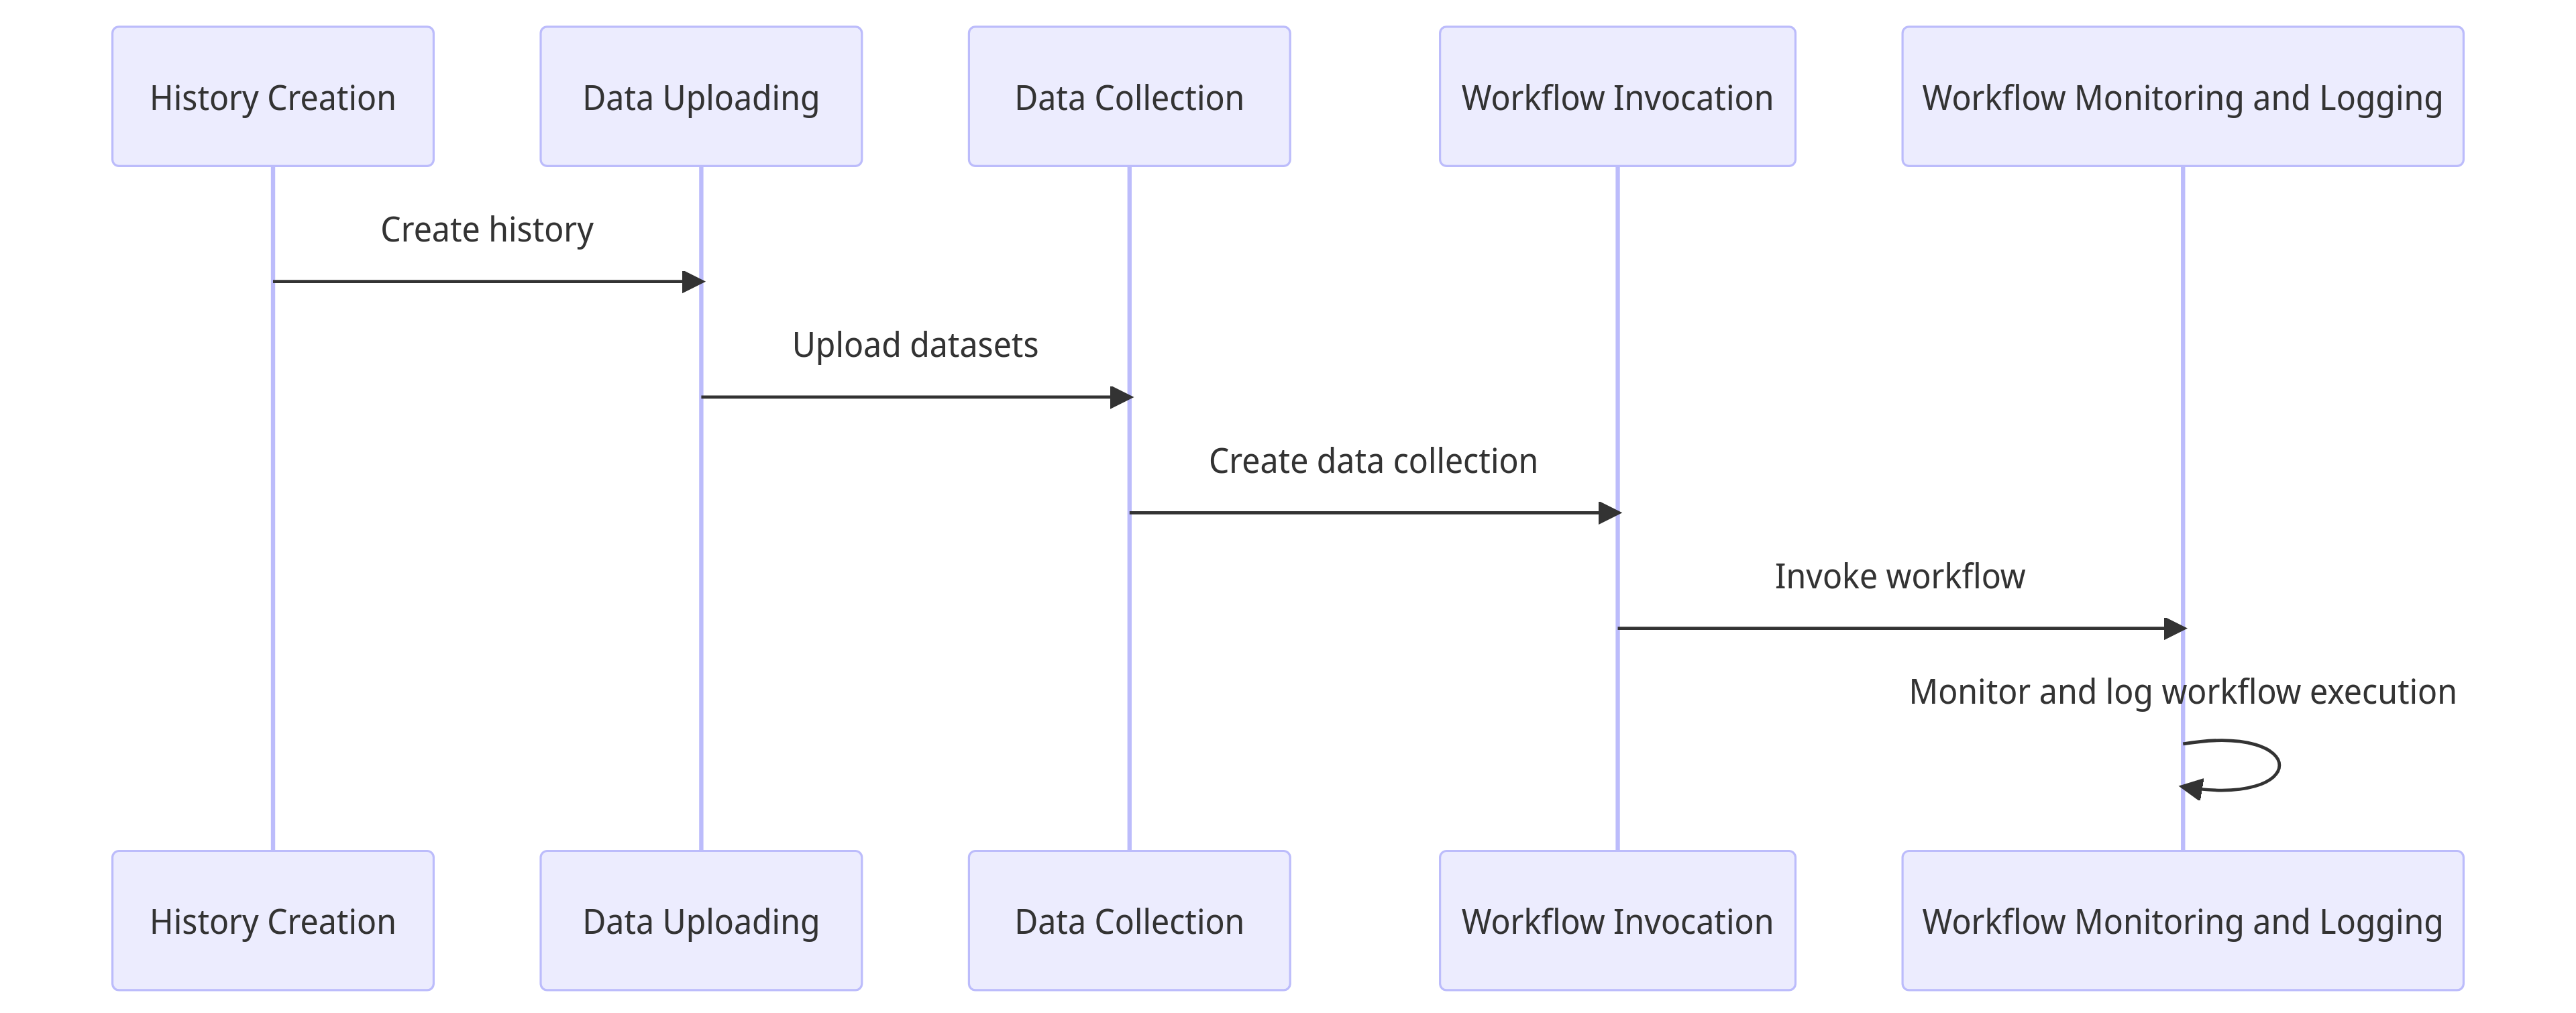
\includegraphics[scale=0.11]{images/evaluation_of_workflows.png}
                \caption{Automation of workflows execution}
                \label{fig:methods:evaluation_of_workflows}
                \small The figure illustrates the automation of workflow execution via Python scripts, leveraging Bioblend. The encompassed steps entail the creation of history, data upload procedures, formulation of data collection, the invocation of the workflow, and diligent workflow monitoring complemented by logging.
            \end{figure}   

            History Creation: In the Galaxy system, the concept of a 'history' denotes a unique computational environment that encapsulates specific datasets and analyses. For every distinct study, the script generates a new history, establishing an isolated workspace for data storage and manipulation. This new history is then associated with its corresponding project ID in a locally stored JSON file, providing easy access for future retrieval.
            
            Data Uploading: The next step in the process involves uploading the project's datasets to the newly created history. This is achieved by forming a single string of the dataset links, which is then uploaded through the upload\_dataset function. This function returns the result of the upload operation, which is further utilized in the subsequent steps. To ensure the robustness of the automation, the script actively monitors the status of the dataset upload operation. If the data is not yet available, the script pauses for a minute before rechecking, thereby preventing premature progression to the next steps.
            
            Data Collection: The datasets are then systematically paired if needed and organized into a Galaxy collection using the create\_paired\_dataset\_collection function. This preparation facilitates efficient downstream analyses by streamlining the data structure.
            
            Workflow Invocation: The datasets having been suitably prepared, the script proceeds to invoke the desired workflow. This is facilitated by mapping the datasets to the inputs of the workflow, identified by its unique ID. The workflow is then run on these datasets within the current history via the gi.workflows.invoke\_workflow function.
            
            Workflow Monitoring and Logging: Perhaps the most crucial step in this automated pipeline is monitoring the execution of the workflow. The updated monitor\_workflow\_execution function keeps track of the workflow status and logs it into a CSV file. This consistent tracking enables the prompt detection of potential issues and the successful completion of the workflow, thereby enhancing the reliability of the process.
            
            By doing these steps, it allows for the efficient handling and processing of multiple projects simultaneously and minimizes manual intervention and potential errors. The scripts for doing these steps are available here \url{https://github.com/YedilSerzhan/beer_microbiome/tree/main/data_plot_n_processing}.


            \subsubsection{Reproducibility analysis}

            This section describes the methodologies and tools used to examine workflow reproducibility, with a particular focus on the three previous studies chosen. I employed \tool{Python} programming language (version 3.9) and \tool{Jupyter Notebook} to conduct the analysis. 
            
            Python libraries \tool{Pandas}\cite{reback2020pandas}, \tool{Matplotlib}\cite{hunter2007matplotlib}, and \tool{Seaborn}\cite{Waskom2021} are utilized for data manipulation and visualization. \tool{Pandas} is a robust and widely used library that offers versatile data structures for efficient data manipulation and cleaning. \tool{Matplotlib} is a highly customizable plotting library that provides a vast array of tools to create high-quality figures for data visualization. \tool{Seaborn}, a statistical data visualization library built on \tool{Matplotlib}, streamlines the creation of informative and attractive plots.
            
            To assess the difference of diversity between original and reproduced data, I applied the Shapiro-Wilk test for normality and the paired-sample t-test, which were implemented using functions from the \tool{scipy.stats} module. The Shapiro-Wilk test is a widely used statistical method for determining if a given dataset is normally distributed. The paired-sample t-test, on the other hand, is employed to compare the means of two related groups, which is particularly useful for assessing the effects of different treatments on a given sample set. The \tool{shapiro} and \tool{ttest\_rel} functions from the \tool{scipy.stats}\cite{2020SciPy-NMeth} module were employed to conduct the Shapiro-Wilk test and paired-sample t-test, respectively. The metrics of the alpha diversity include Chao1, Shannon, and Simpson. Chao1 metric primarily estimates species richness, which is the number of different species present in a sample. Shannon Index encapsulates both species richness and evenness within a community. While also capturing species richness and evenness, the Simpson Index places more weight on the most abundant species.
            
    \subsection{Beer microbiome database: BeerMicroDB}

        The results generated from the analysis of beer data samples collected using the workflows mentioned above serve as the foundation for the beer microbiome database, MicroBeerDB.

        \subsubsection{Database implementation}

        
        \begin{figure}[H]
            \centering
            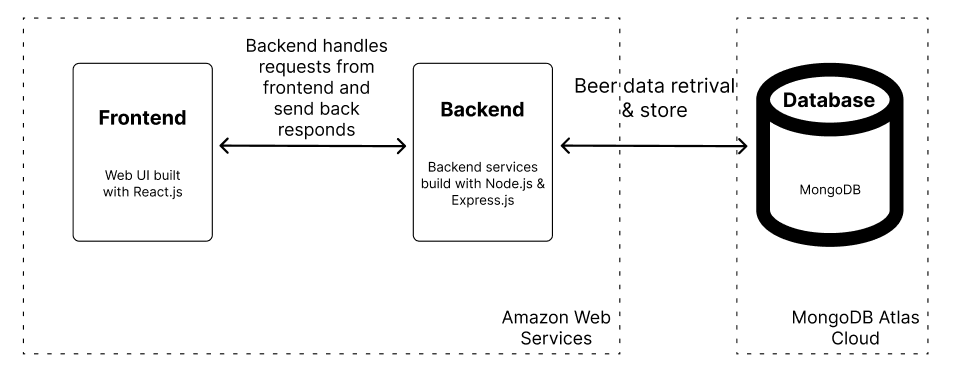
\includegraphics[scale=0.5]{images/system_architecture.png}
            \caption{The system architecture diagram of BeerMicroDB}
            \small The frontend of BeerMicroDB is constructed using React.js. Resources for this frontend are sourced from requests to the backend, developed with Express.js. This backend interfaces with a database established in MongoDB. Both the frontend and backend are deployed on Amazon Web Services, while the database resides on the MongoDB Atlas Cloud.
            \label{fig:methods:system_architecture}
        \end{figure}   

        The MicroBeerDB consists of 3 parts: 1. a frontend website built with React.js providing a web user interface. 2. Backend services built with Node.js and Express.js providing API services. 3. MongoDB hosted on MongoDB Atlas Cloud to store required data.

        \paragraph*{Frontend implementation}

            The frontend implementation of the Beer Microbiome Database website is primarily built using React, a powerful JavaScript library for constructing user interfaces, along with Material-UI, a popular React UI framework.

            \begin{figure}[H]
                \centering
                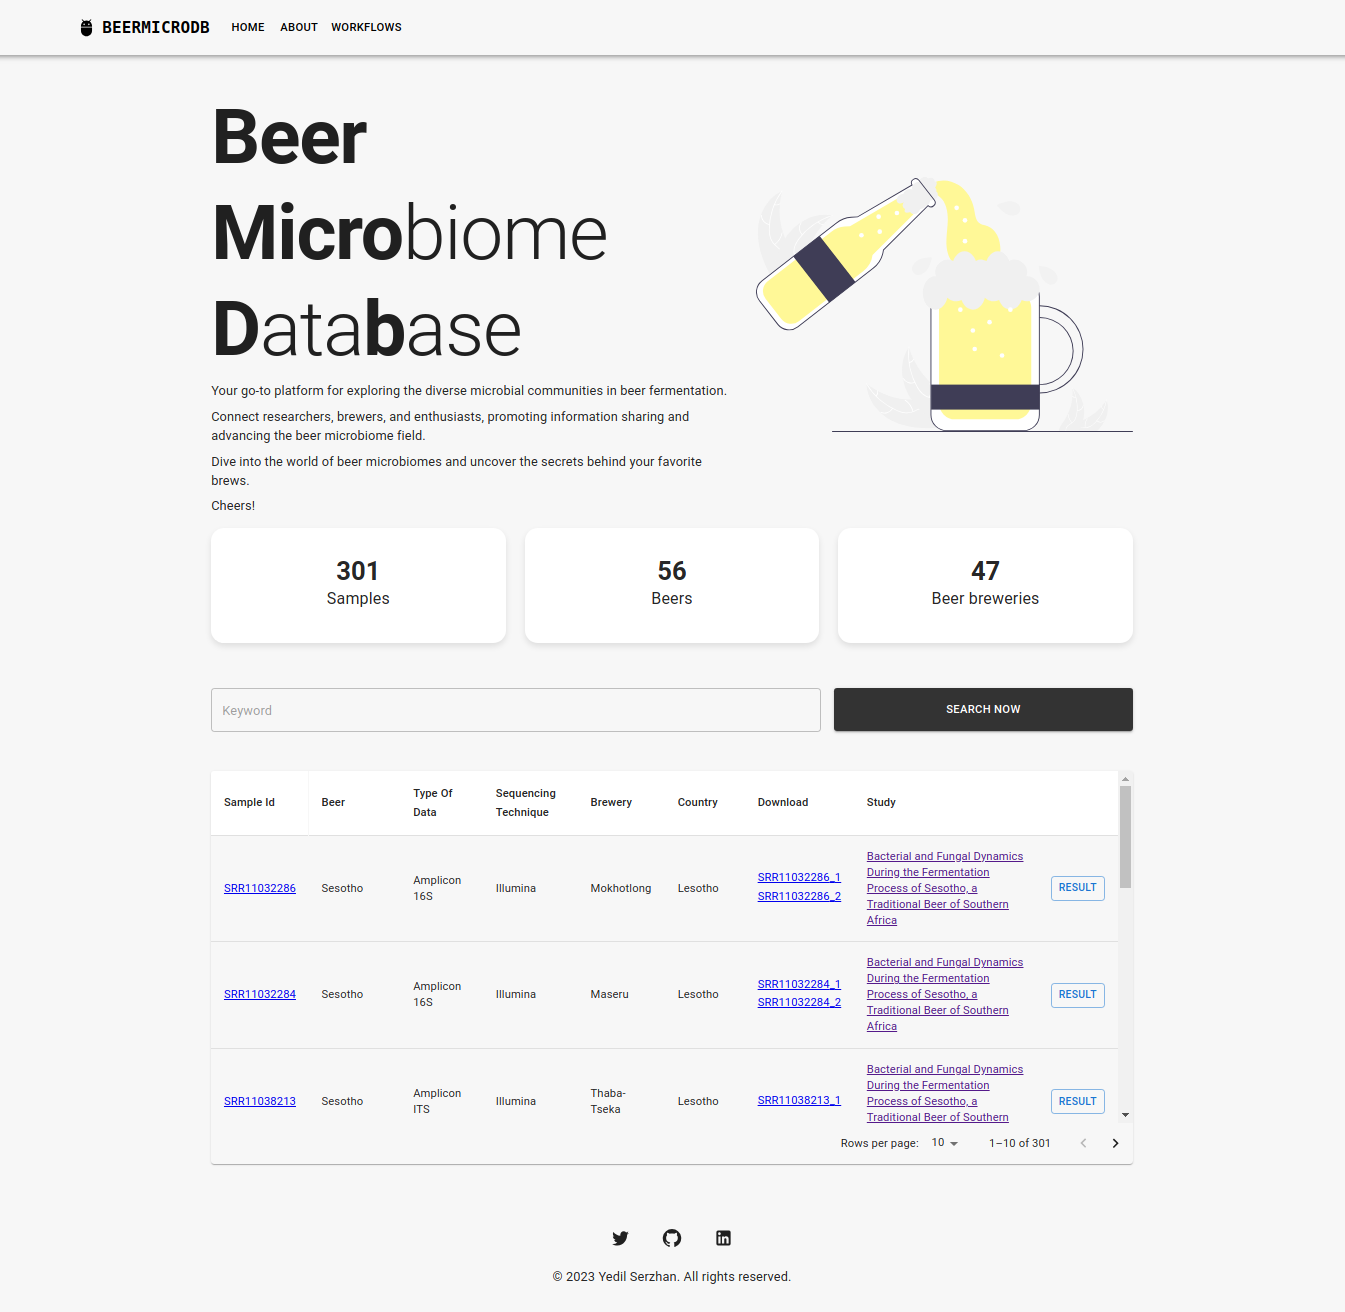
\includegraphics[scale=0.3]{images/home_page.png}
                \caption{BeerMicroDB Home page}
                \small The homepage features a welcoming and explanatory message accompanied by an image of beer at the top. This is followed by a section presenting statistics pertaining to BeerMicroDB. Further down, a search bar allows users to seek specific information, with the results displayed in a table format beneath it.
                \label{fig:methods:beermicrodb_home_page}
            \end{figure}  

            The Home page shown in figure \ref{fig:methods:beermicrodb_home_page} serves as the primary entry point to the application. Here, a combination of Material-UI components is used to create a visually appealing layout. The Home page contains a search bar, and a table constructed using Material-UI components displaying various microbiome samples. This page makes an asynchronous fetch request to a server upon mount to retrieve the microbiome sample data. This data is then managed using the useState and useEffect hooks from React to implement a search functionality, allowing users to filter through the microbiome samples based on their search criteria. The sample table includes pagination, offering a user-friendly way to navigate through potentially large sets of data. Each row in the table represents a single sample and provides a link to the study page that the sample belongs to. 

            The Study page, a dynamic component of the application, employs React Router's useParams hook to capture the study ID from the URL. This ID is subsequently used to dynamically import corresponding study results. This page shows the community profiling result at the species level for each sample belonging to the study.
            
            The About page delivers valuable insights about the project's purpose, context, methodologies, and data sources. The Workflows page exhibits the shotgun and metabarcoding sequencing workflow diagram, elucidating the process involved in analyzing the microbiome samples.
            
            All pages have a consistent layout and are equipped with a navigation bar and a Footer component, providing guidance to different components of the website. It utilizes the BrowserRouter, Routes, and Route components from the react-router-dom library to handle the navigation between different parts of the website.
                        
            In summary, the tech stack for the Beer Microbiome Database frontend implementation allows for the creation of dynamic, interactive web pages. And it provides a smooth user experience. The user interface is divided into distinct components, promoting the reusability and maintainability of the code. The frontend code base is available at \url{https://github.com/YedilSerzhan/beer_microbiome/tree/main/frontend}. 

        
        
        \paragraph*{Backend implementation}
        
            The backend is built with Express, a minimalistic and flexible Node.js web application framework, coupled with the Mongoose library for MongoDB \cite{banker2016mongodb}. 

            \begin{figure}[H]
                \centering
                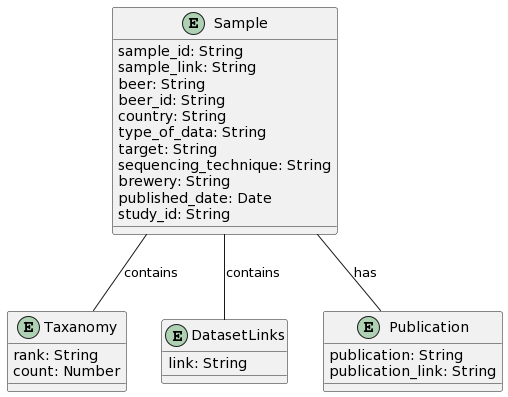
\includegraphics[scale=0.5]{images/db_model.png}
                \caption{Database models}
                \small In the MongoDB, the sample document model encompasses both metadata and the outcomes of microbiome analysis pertinent to each respective sample.
                \label{fig:methods:db_model}
            \end{figure}   
        
            The mongoose-based 'Sample' schema illustrated in figure \ref{fig:methods:db_model} stands as the cornerstone of our database model. This schema was carefully designed to accommodate a plethora of attributes intrinsic to the beer microbiome samples, such as 'sample\_id', 'beer', 'brewery', 'taxonomy', and more. Notably, 'taxonomy' is an array of objects, capturing information on various taxonomic ranks and their respective counts - a fitting representation of the complexity of microbiome data. In addition to these, the model carries metadata attributes including 'sequencing\_technique', 'country', 'published\_date', 'dataset\_links', and more, thereby encapsulating the diverse spectrum of data associated with each microbiome sample.
            
            The implementation of RESTful API operations is achieved through distinct route handlers for each HTTP method (GET, POST, PUT, DELETE). Each route corresponds to a specific action - obtaining all samples, getting a single sample, creating a new sample, updating an existing sample, and deleting a sample. The utilization of asynchronous functions in each route ensures non-blocking code execution.

            The backend code base is available at \url{https://github.com/YedilSerzhan/beer_microbiome/tree/main/backend}. 
                
        \subsubsection{Data ingestion}

        Data ingestion is the process of populating a database. In our case, we need to populate the results of workflows on the beer sample data to the microbiome database we are building.

        Firstly we perform data preprocessing on a DataFrame 'df' that contains the beer microbiome result. The taxonomy, dataset\_links, and publication related to the sample are objectified and saved to 'db\_ready.json', ready for ingestion.
                
        Then a code snippet initiates the later process by setting up a connection with the MongoDB database using the 'mongoose' library. Once the connection is established, the 'fs' (File System) module reads the 'db\_ready.json' file, containing the data to be populated. The JSON file is read asynchronously to prevent the blocking of subsequent operations.
        
        Each object in the JSON array is instantiated as a 'Sample' model, which is defined by the 'Sample' schema in Mongoose. This operation ensures that the data being saved adheres to the structure and validation rules defined in the schema. A save operation is then executed asynchronously on the instantiated 'Sample' model. If the save operation is successful, a console message confirming the ID of the saved record is printed. Otherwise, an error message is logged.
        
        In this way, the beer microbiome results are populated into the database. The scripts to do the data ingestion can be accessed at \url{https://github.com/YedilSerzhan/beer_microbiome/tree/main/backend/data}.
        
\section{Results}

The results section is divided into two subsections. The first subsection presents the reproduced results from three previous beer microbiome studies that were introduced earlier, along with a comparison between the reproduced results and the original findings. The second subsection provides an overview of BeerMicroDB, where the overall fungal and bacterial microbiome results from the beer samples are presented.

\subsection{Results of reproducibility analysis}

Here are the reproduced results and comparisons between them and the original results from the prior three beer microbiome studies respectively.

\subsubsection{BeerDeCoded: the open beer metagenome project}

    In the BeerDecoded project \cite{sobel2017beerdecoded}, as shown in the figures \ref{fig:results:BeerDecoded_beer_variety}, analysis of 39 ITS samples revealed a total of 20 distinct fungal species, fewer than the 42 species identified in the larger scope of the BeerDEcoded study. The beer sample exhibiting the greatest ITS diversity, comprising 6 unique fungal species, was the Waldbier 2014 Schwarzkiefer. This observation aligns with the general trend observed in the BeerDEcoded project, albeit with fewer species when compared to the maximum of 19 identified in a single sample there. Four other beers, namely Stirling, La Fourbe and BE from Switzerland, and Chimay Red Cap from Belgium, also exhibited high ITS diversity with 5 species each, showing a notable variety of ITS compared to other samples within the BeerDEcoded project.

\begin{figure}[H]
    \centering
    \begin{subfigure}[b]{0.45\textwidth}
        \centering
        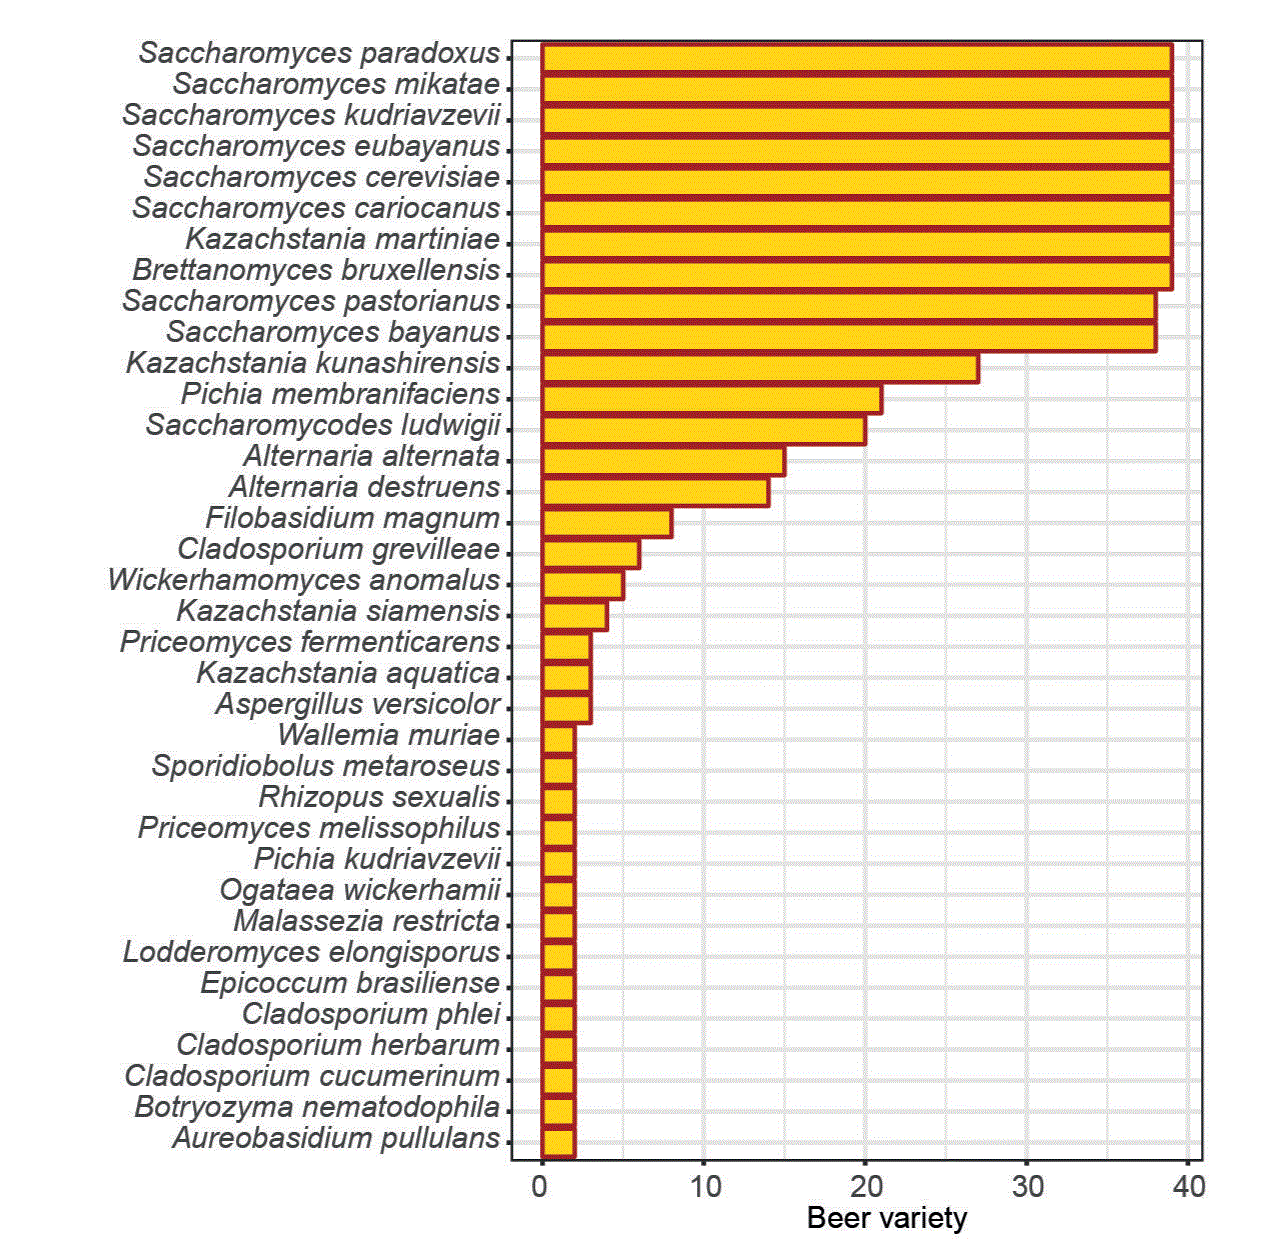
\includegraphics[width=\textwidth]{images/orginal_BeerDEcoded_beer_variety.png}
        \caption{Orginal result}
        \label{fig:results:orginal_BeerDecoded_beer_variety}
    \end{subfigure}
    \hfill
    \begin{subfigure}[b]{0.45\textwidth}
        \centering
        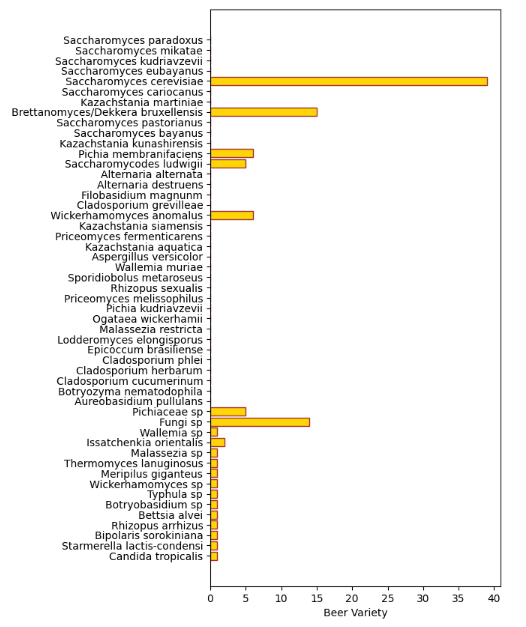
\includegraphics[width=\textwidth]{images/BeerDEcoded_beer_variety.png} 
        \caption{Reproduced results}
        \label{fig:results:reproduced_BeerDecoded_beer_variety}
    \end{subfigure}
    \caption{BeerDecoded beer variety diagram}
    \small The figures present data regarding the quantity of beers associated with each species identified in both the original and reproduced results. For clarity, the figure depicting the reproduced results on the right retains the species order as presented in the original figure. This arrangement aids in a more transparent comparison between the two sets of results.
    \label{fig:results:BeerDecoded_beer_variety}
\end{figure}


    Upon examining the heatmap \ref{fig:results:BeerDecoded_heatmap}, we observe, as expected, that \textit{Saccharomyces} is the most prevalent species, identified in every beer sample, a finding that is in line with the broader BeerDEcoded project results. The next most common species is \textit{Brettanomyces bruxellensis}, appearing in 15 samples, a species found in all samples within the BeerDEcoded project. Unexpectedly, an organism labeled as \textit{Fungi sp} is also found in high abundance. Further investigation revealed that \textit{Fungi sp} is labeled as 'unidentified' in the database. At present, we are uncertain whether this status is due to the workflow's inability to accurately identify it as a known species, or if it truly remains unclassified in the database.

    \begin{figure}[H]
        \centering
        \begin{subfigure}[b]{0.6\textwidth}
            \centering
            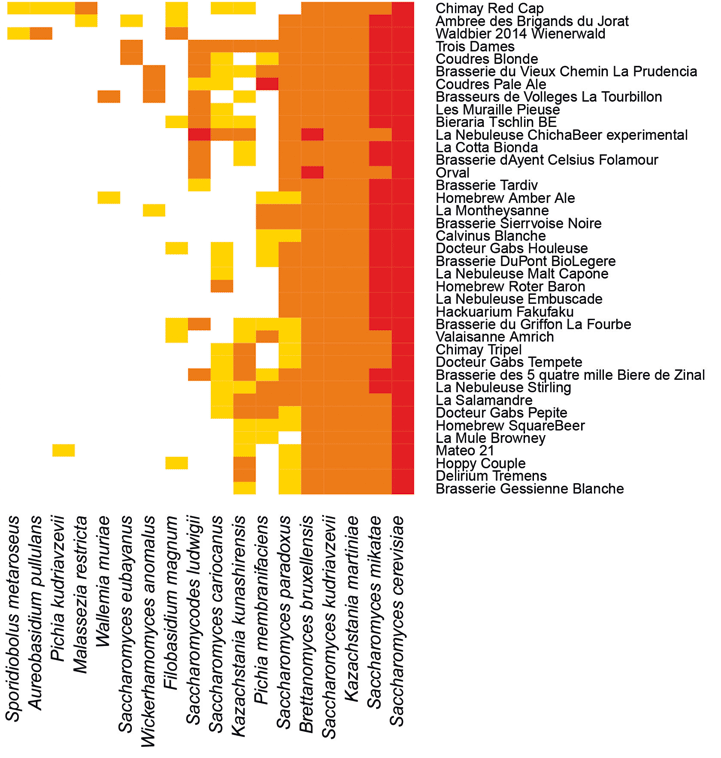
\includegraphics[width=\textwidth]{images/beerdecoded/orginal_beerDecoded_heatmap.png}
            \caption{Original results}
            \label{fig:results:oringal_BeerDecoded_heatmap}
        \end{subfigure}
        \hfill
        \begin{subfigure}[b]{0.6\textwidth}
            \centering
            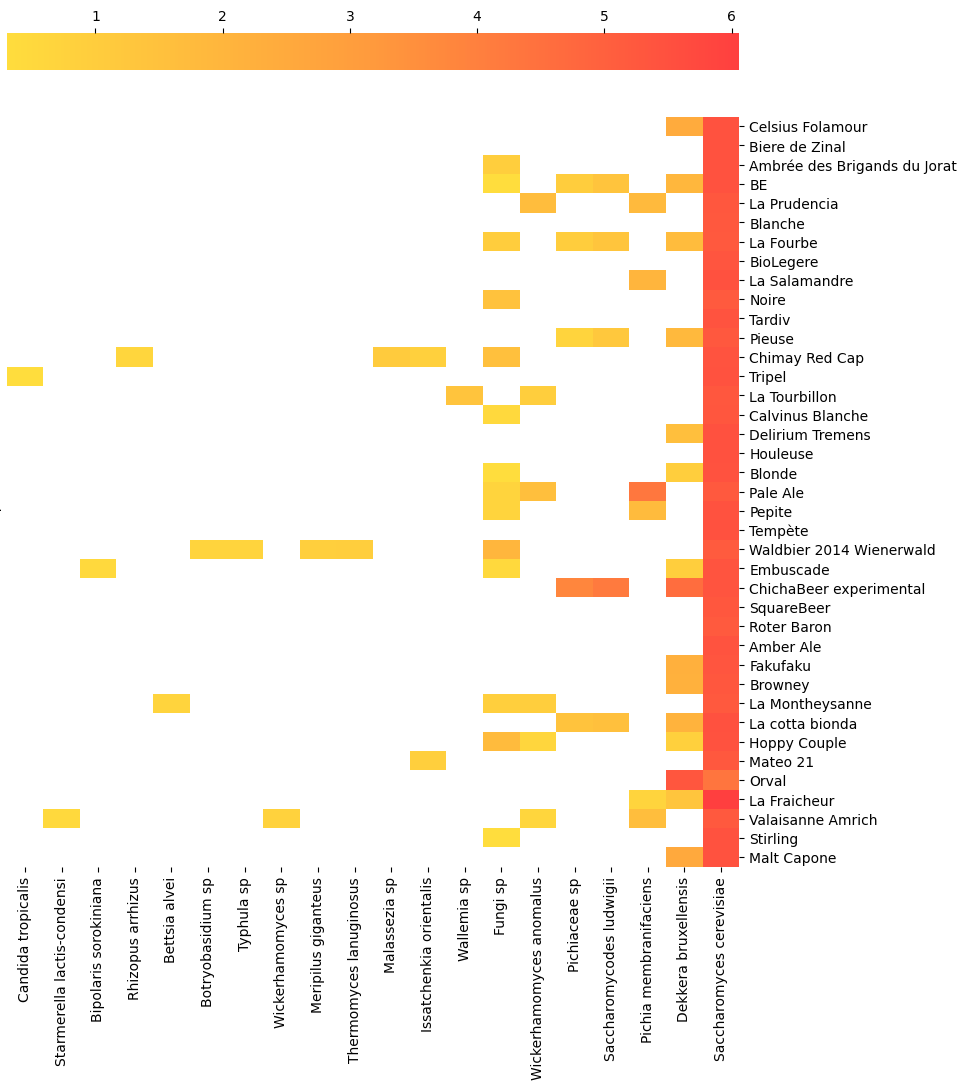
\includegraphics[width=\textwidth]{images/beerdecoded/BeerDecoded_heatmap.png}
            \caption{Reproduced results}
            \label{fig:results:reproduced_BeerDecoded_heatmap}
        \end{subfigure}
        \caption{Heatmap of the number of reads per ITS per beer}
        \small Beer names are shown on the right and species names are shown at the bottom.
        \label{fig:results:BeerDecoded_heatmap}
    \end{figure}
    
    In contrast to the BeerDecoded project, our analytic process was unable to detect 31 species that were identified in the BeerDecoded study. However, we did discover 7 species not previously identified. This discrepancy could potentially stem from the relatively low quality of the samples, which averaged a quality score of around 20. As we utilized the QIIME 2 and BLAST consensus methodologies for taxonomy classification, the less-than-ideal quality could lead to ambiguous results. In instances where one feature sequence may be linked to more than two species, it could result in the feature being labeled as unidentified. This classification approach is notably different from the strategy adopted in the BeerDecoded study. In the latter, they followed an unconventional methodology of constructing a database with assumed taxonomies presumed to be present in the samples. They then proceeded to map the sequences directly to their custom-built database.

\subsubsection{Bacterial and Fungal Dynamics During the Fermentation Process of Sesotho, a Traditional Beer of Southern Africa}

    % \begin{figure}[H]
    %     \centering
    %     \includegraphics[scale=0.7]{images/sesotho_species_relative_abundance.png}
    %     \caption{Sesotho species relative abundance}
    %     \label{fig:methods:sesotho_species_relative_abundance}
    % \end{figure}


     The collection of Sesotho samples took place from five different districts (breweries) namely, Maseru (MSU), Mafeteng (MFT), Thaba-Tseka (HN), Butha-Buthe (Butha), and Mokhotlong (MK). Within each location, five samples were obtained, representing various stages of fermentation. The first sample (1) was gathered one hour after the initial starter culture was added to commence the first fermentation phase. Subsequently, the second sample (2) was obtained at approximately eight hours into the fermentation process, after the completion of the first fermentation phase. The third sample (3) was collected one hour after introducing the second starter culture, which initiated the second and final fermentation phase. Following that, the fourth sample (4) was acquired approximately eight hours after the second fermentation, prior to the beer undergoing sieving, which involves the separation of sorghum malt from the beer. Lastly, the fifth sample (5) was taken from the final product, around eight hours into the maturation stage.
    
    Figures \ref{fig:results:sesotho_phyla_relative_abundance}, \ref{fig:results:sesotho_family_relative_abundance}, and \ref{fig:results:sesotho_genus_relative_abundance}, presented in this thesis and the original study, respectively, depict the distribution of fungal taxa in Sesotho beer at the Phylum, Family, and Genus levels.

    \begin{figure}[H]
        \centering
        \begin{subfigure}[b]{1\textwidth}
            \centering
            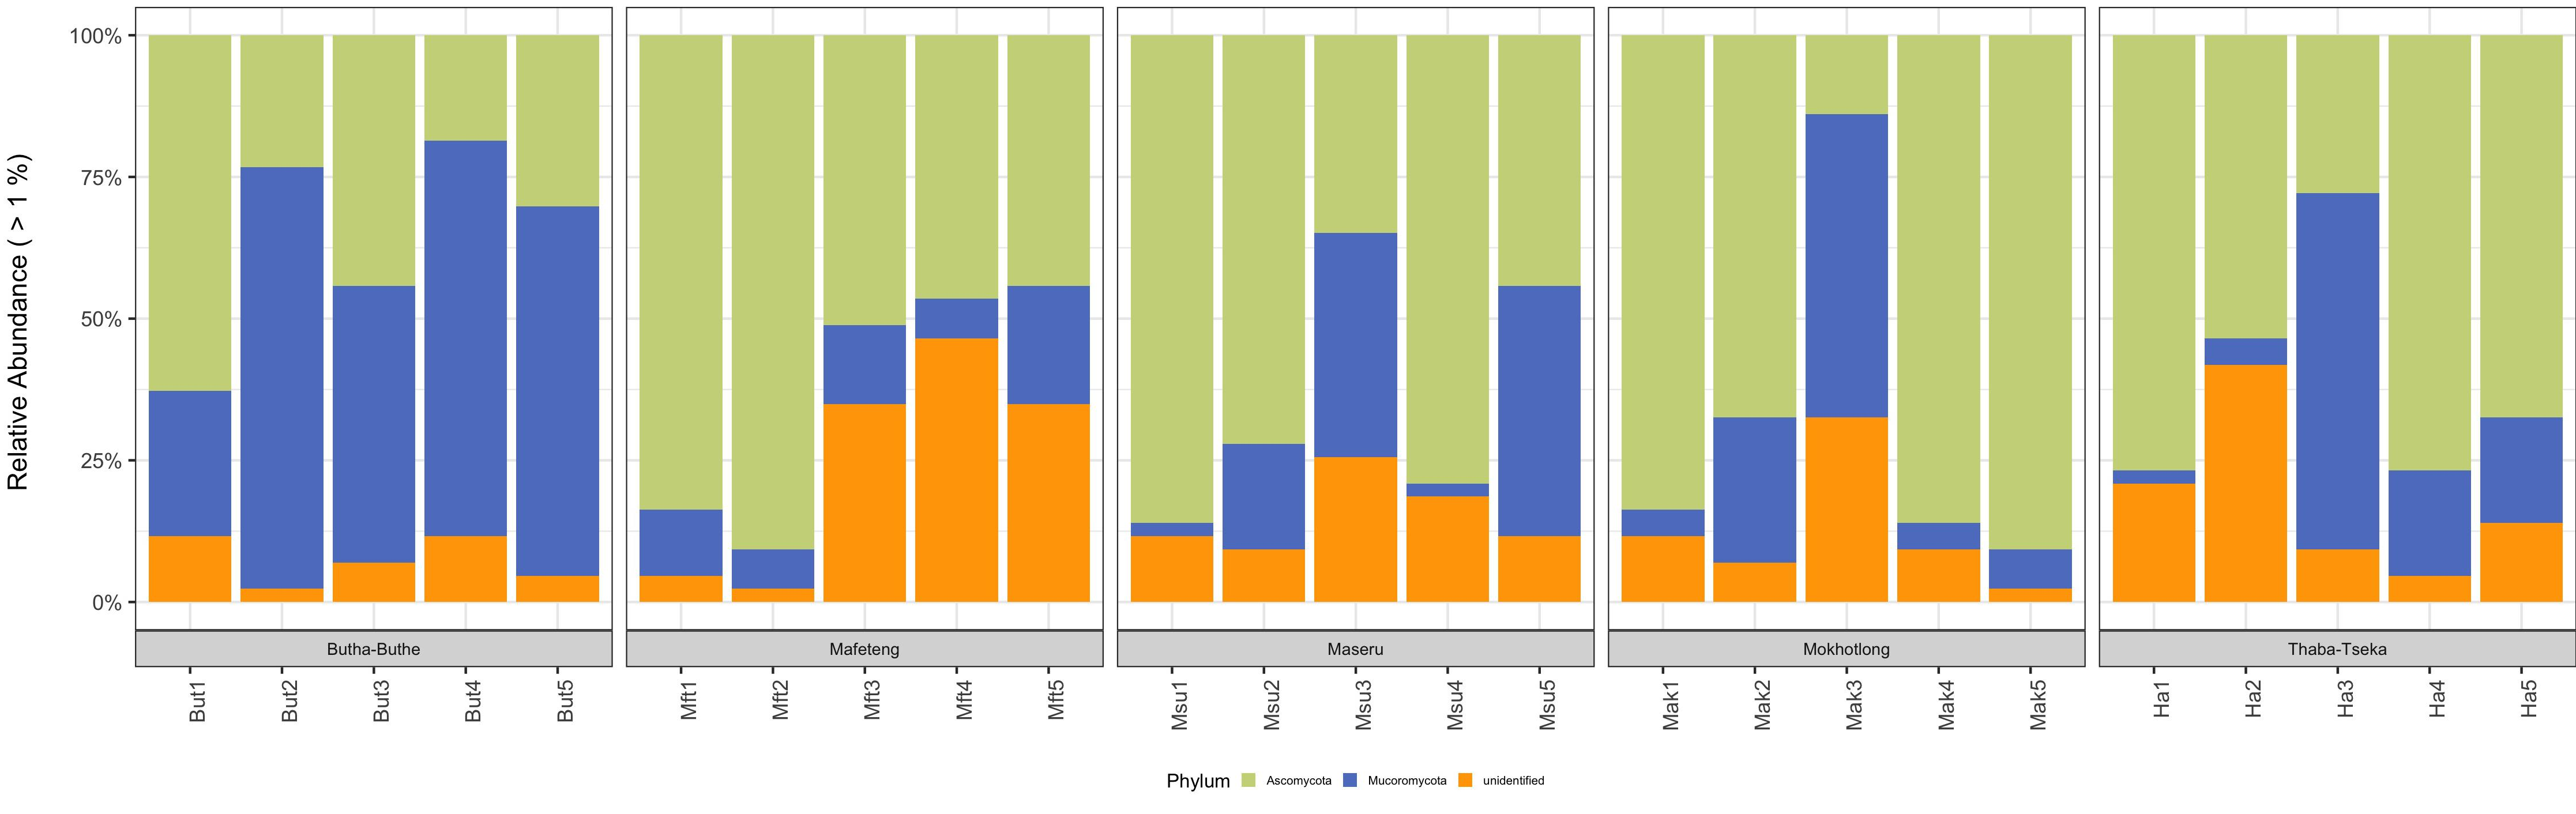
\includegraphics[width=\textwidth]{images/sesotho/original_sesotho_phyla_relative_abundance.png}
            \caption{Original results}
            \label{fig:results:original_sesotho_phyla_relative_abundance}
        \end{subfigure}
        \hfill
        \begin{subfigure}[b]{1\textwidth}
            \centering
            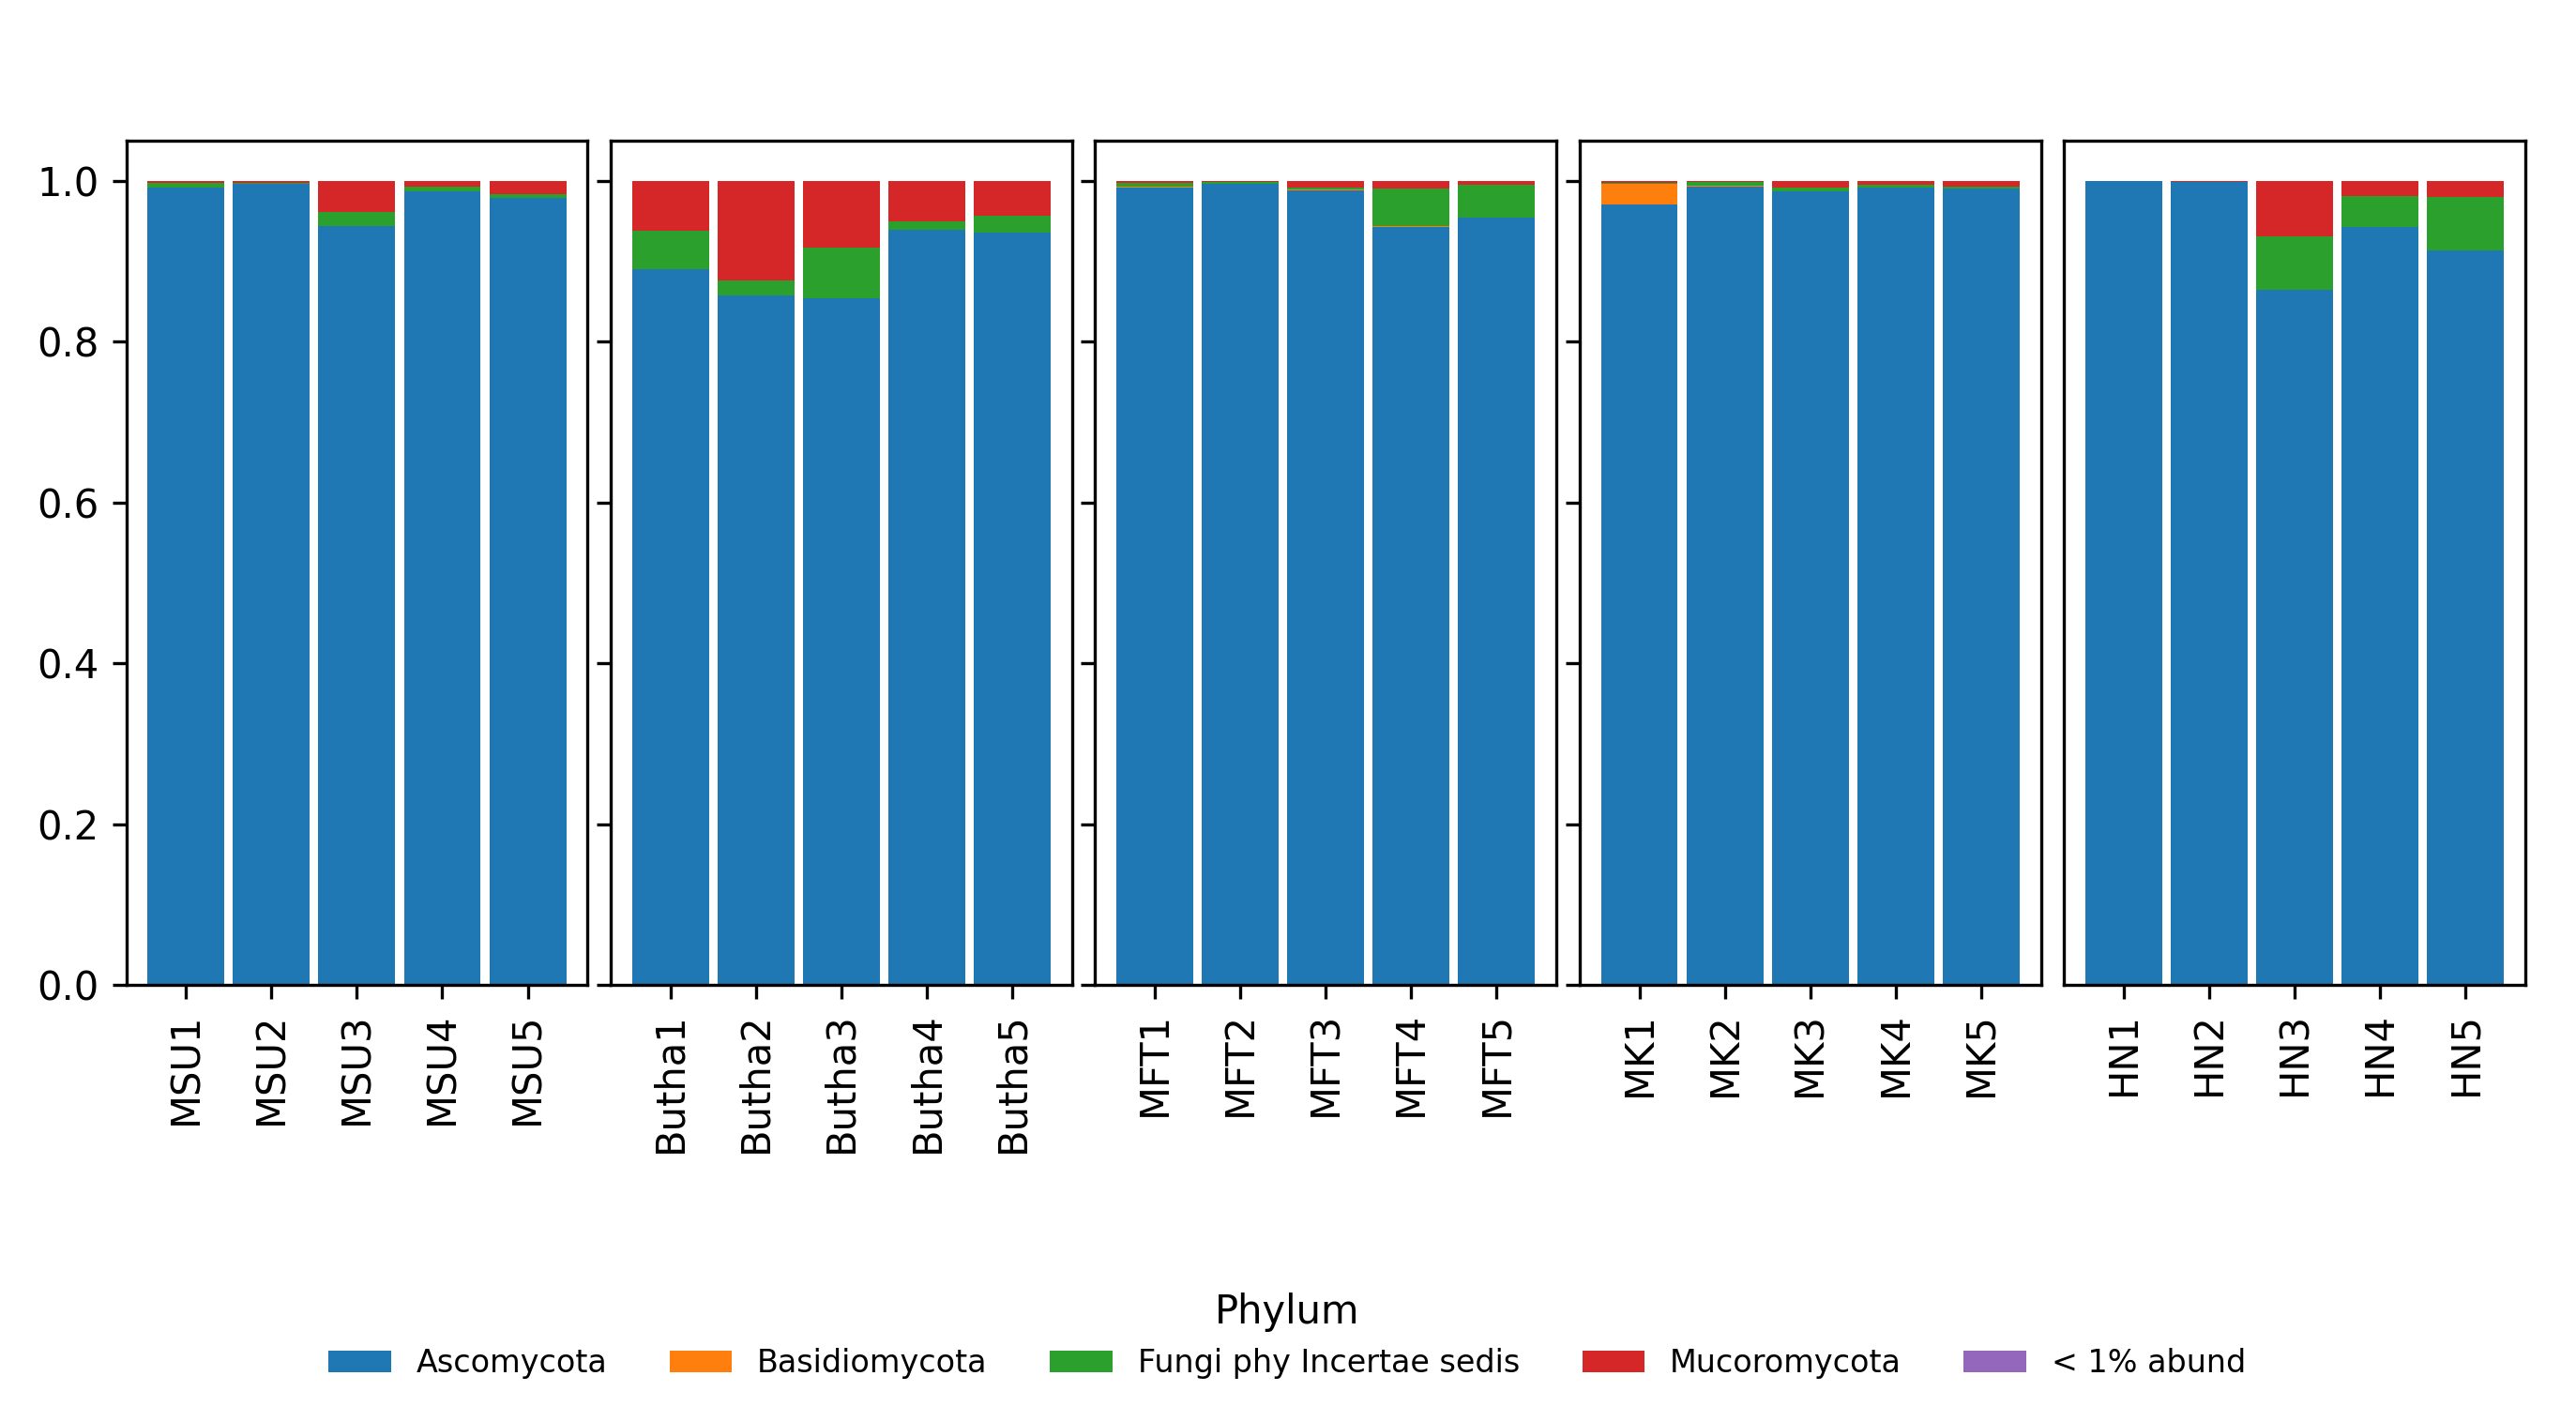
\includegraphics[width=\textwidth]{images/sesotho/sesotho_phyla_relative_abundance.png}
            \caption{Reproduced results}
            \label{fig:results:reproduced_sesotho_phyla_relative_abundance}
        \end{subfigure}
        \caption{Distribution of fungal Phylum in Sesotho.}
        \small In the graphical representation, the x-axis delineates the various breweries, labeled as Maseru (MSU), Mafeteng (MFT), Thaba-Tseka (HN), Butha-Buthe (Butha), and Mokhotlong (MK). To illustrate, the label "MK1" denotes a sample sourced from Mokhotlong during the first stage of fermentation. The fungal phyla Ascomycota and Mucoromycota emerged as the predominant groups in the study. Notably, Ascomycota displayed a higher dominance in the reproduced results compared to the original findings.
        \label{fig:results:sesotho_phyla_relative_abundance}
    \end{figure}
    
    Similar to the original findings, Ascomycota and Mucoromycota were the predominant fungal phyla observed in all samples and locations as shown in figure \ref{fig:results:sesotho_phyla_relative_abundance}. However, in this thesis, the presence of Basidiomycota was also identified. Basidiomycota fungi are widely distributed in nature and can be found in various habitats such as soil, plants, and air. If the raw ingredients, such as sorghum or maize, are contaminated with Basidiomycota spores during the brewing process, these spores can enter the beer mixture and subsequently proliferate during fermentation.

        \begin{figure}[H]
        \centering
        \begin{subfigure}[b]{1\textwidth}
            \centering
            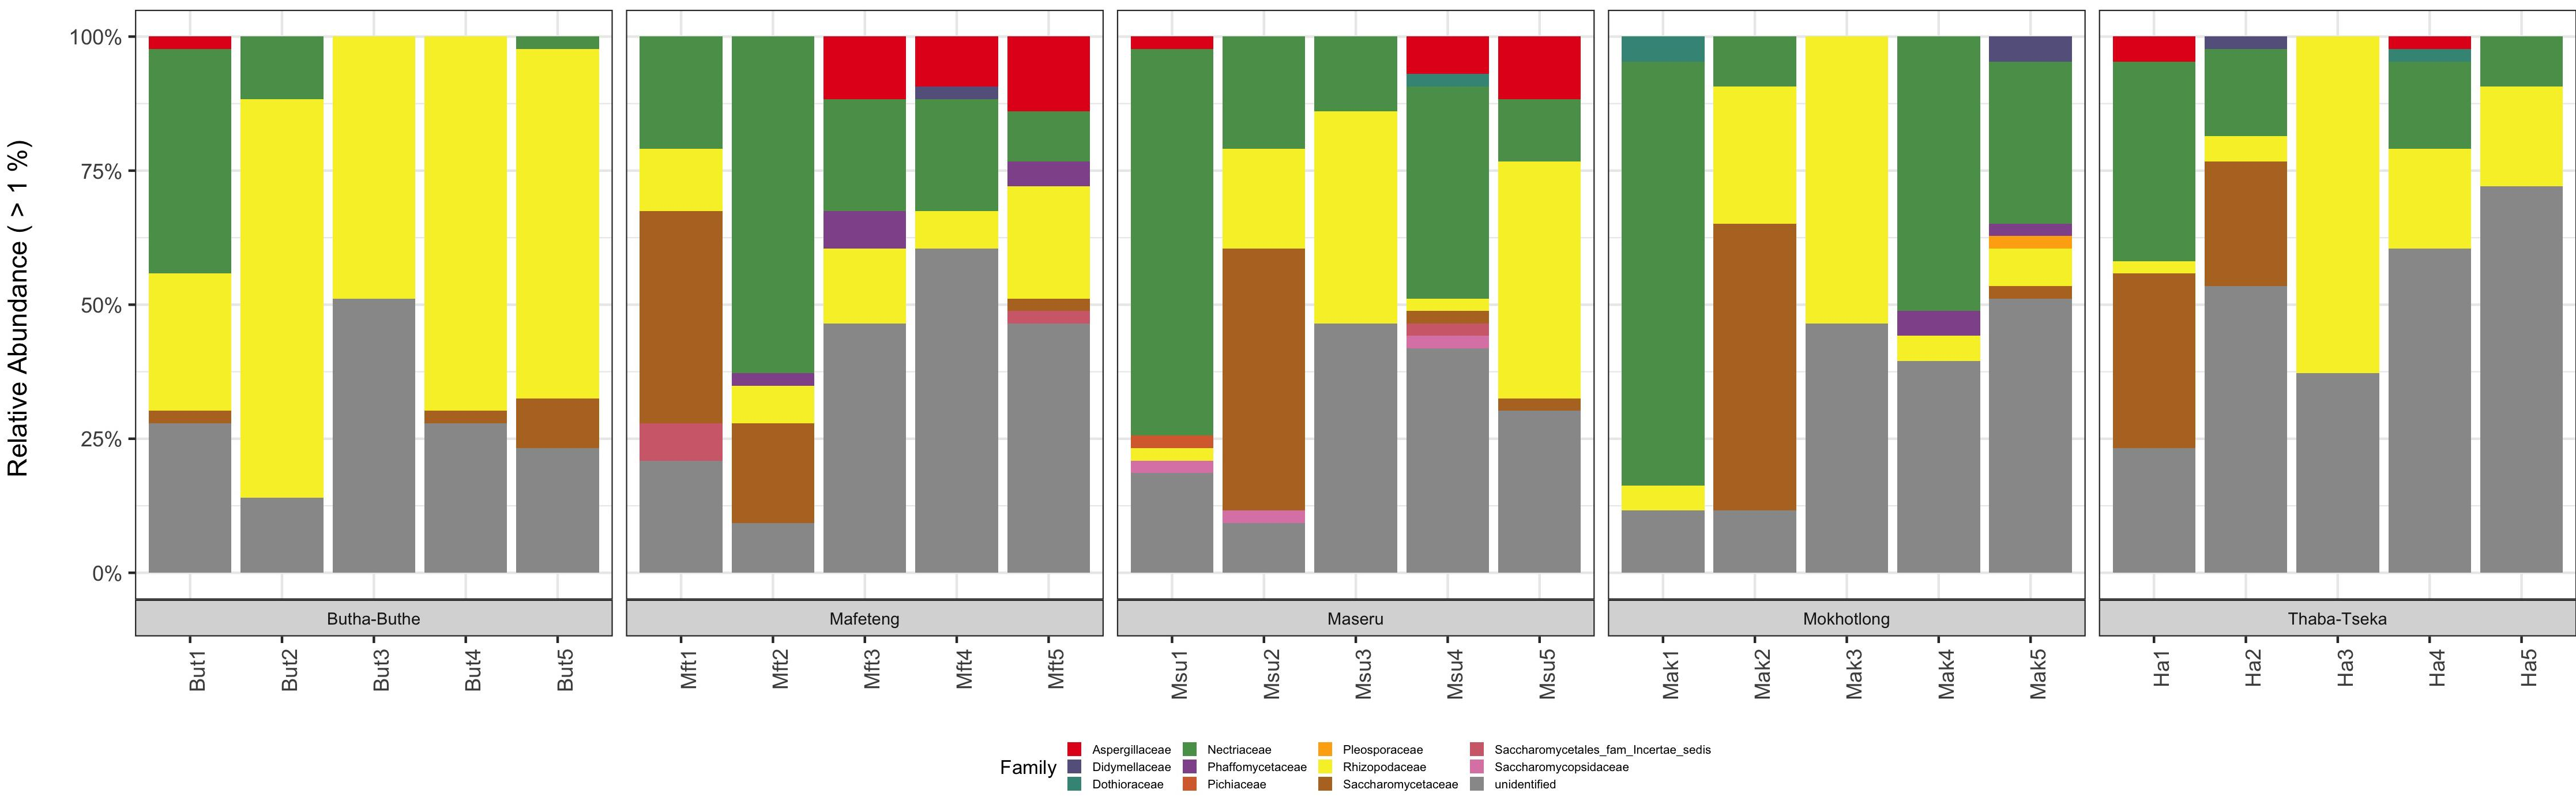
\includegraphics[width=\textwidth]{images/sesotho/original_sesotho_families_relative_abundance.png}
            \caption{Original results}
        \end{subfigure}
        \hfill
        \begin{subfigure}[b]{1\textwidth}
            \centering
            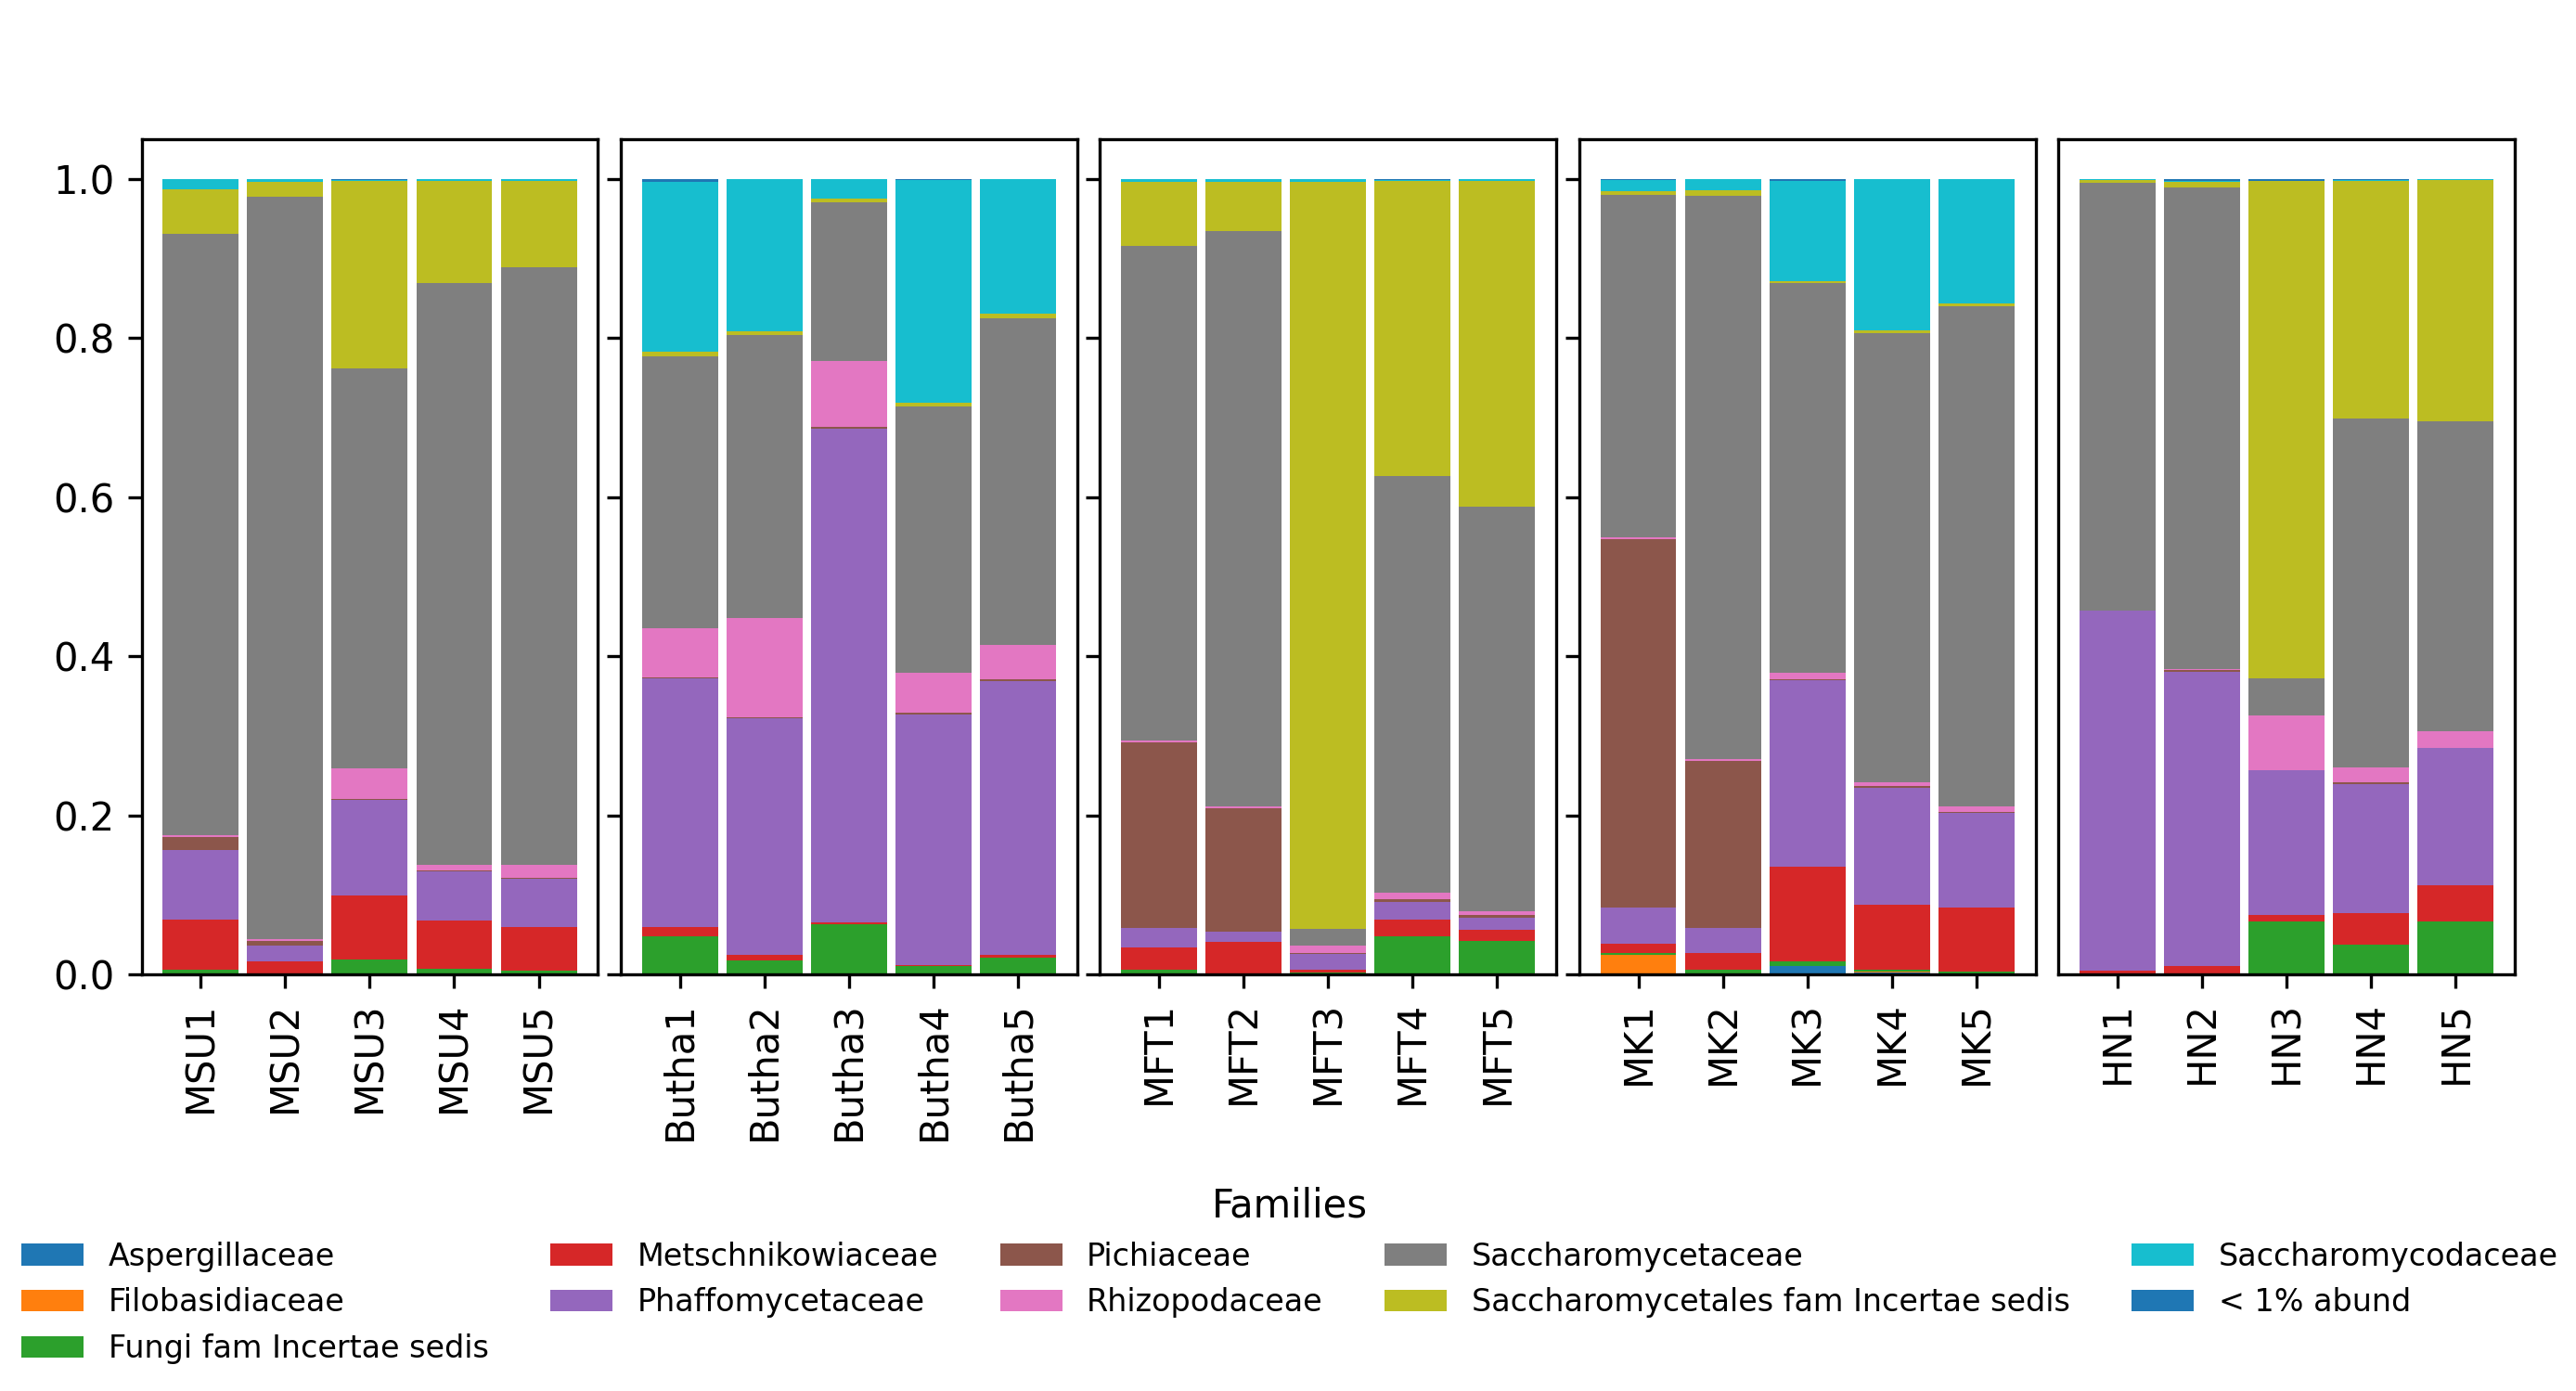
\includegraphics[width=\textwidth]{images/sesotho/sesotho_family_relative_abundance.png}
            \caption{Reproduced results}
        \end{subfigure}
        \caption{Distribution of fungal Family in Sesotho.}
        \small In alignment with the original findings, the reproduced data also identified the presence of \textit{Phaffomycetaceae} and \textit{Pichiaceae}.
        \label{fig:results:sesotho_family_relative_abundance}
    \end{figure}
    
    As seen in figure \ref{fig:results:sesotho_family_relative_abundance}, consistent with the Original results, we observed the presence of \textit{Saccharomycetaceae} and \textit{Nectriaceae} from the Phylum Ascomycota, as well as \textit{Rhizopodaceae} from the Phylum Mucoromycota. Additionally, we detected a substantial abundance of \textit{Phaffomycetaceae} and \textit{Pichiaceae}, which are families of yeasts belonging to the order Saccharomycetales.

    \begin{figure}[H]
        \centering
        \begin{subfigure}[b]{1\textwidth}
            \centering
            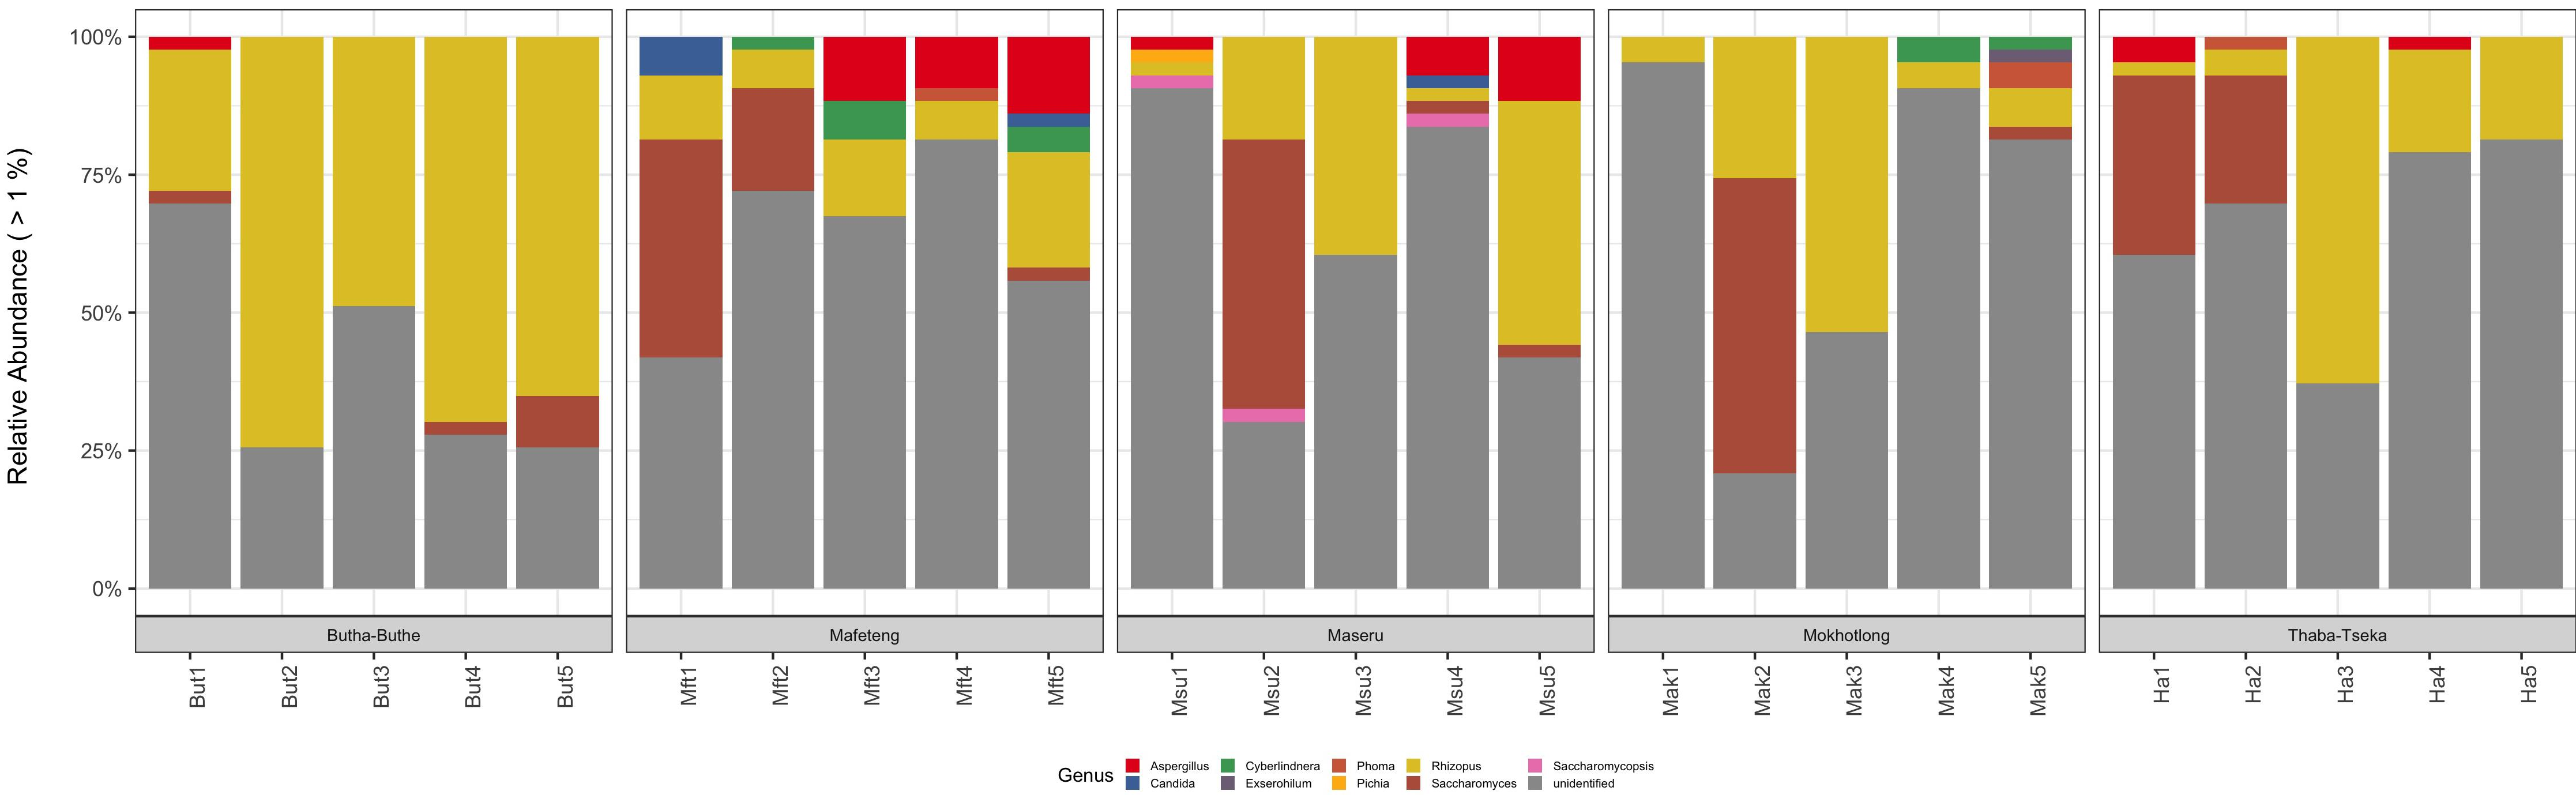
\includegraphics[width=\textwidth]{images/sesotho/original_sesotho_genera_relative_abundance.png}
            \caption{Original results}
        \end{subfigure}
        \hfill
        \begin{subfigure}[b]{1\textwidth}
            \centering
            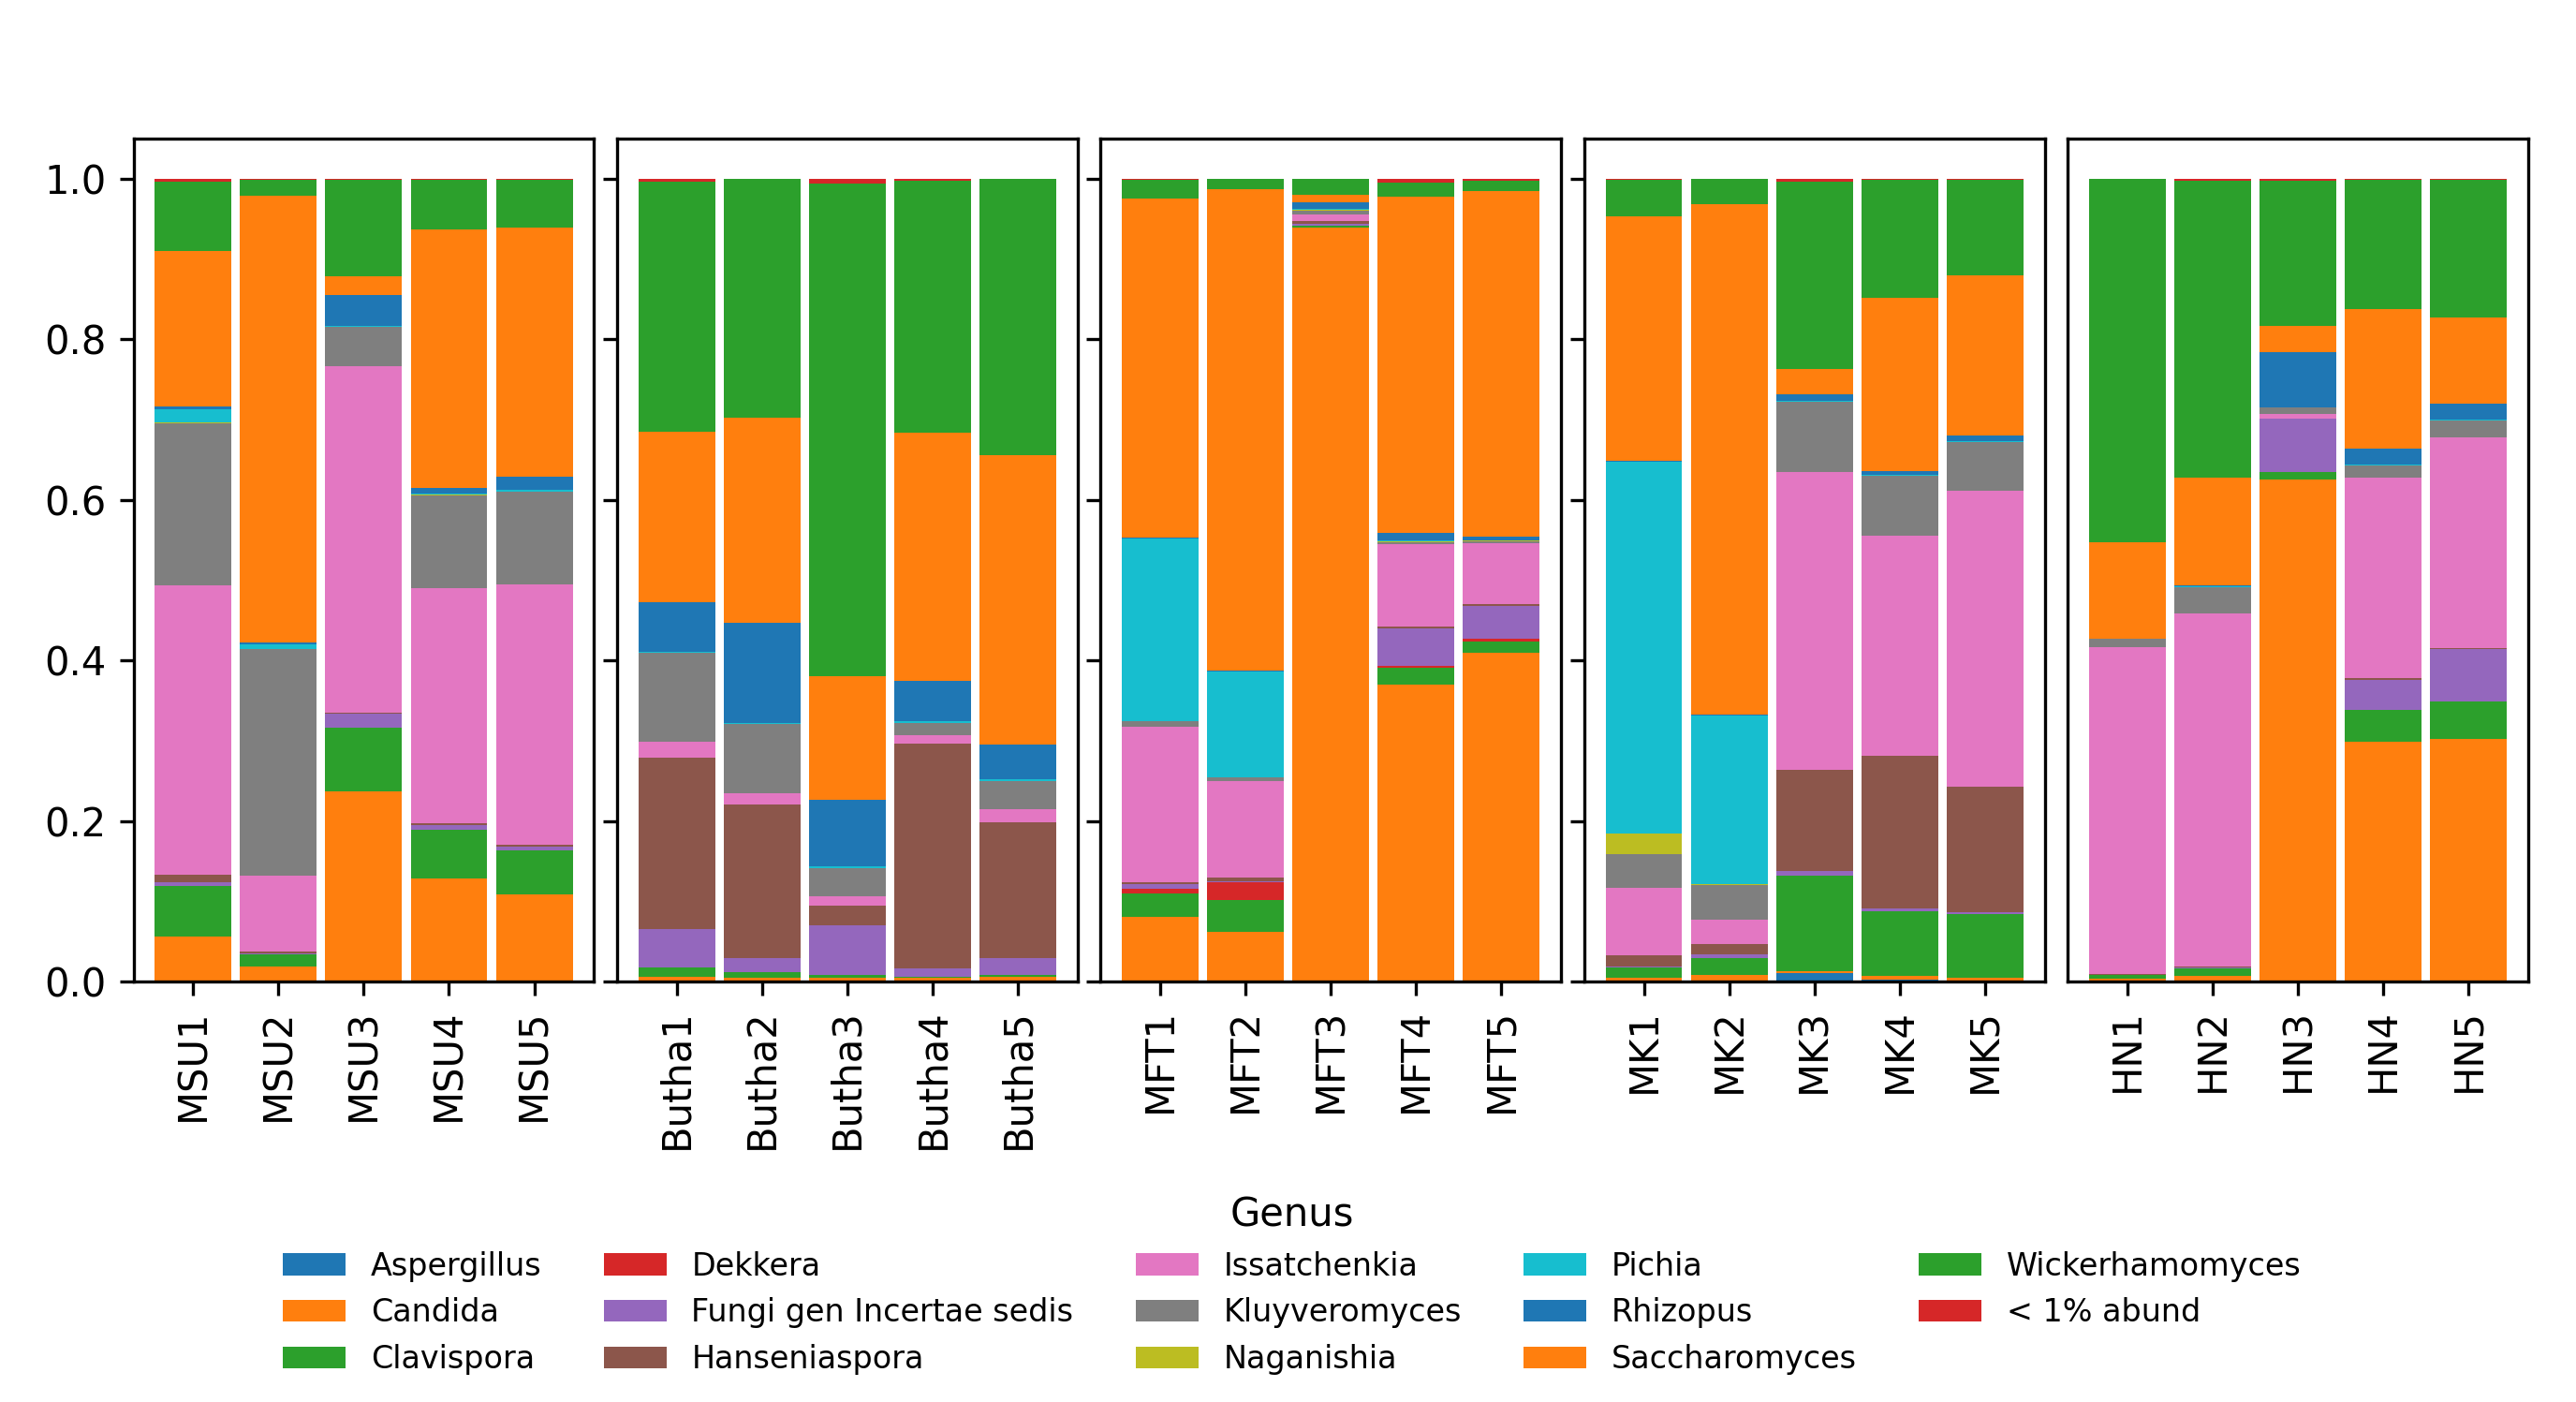
\includegraphics[width=\textwidth]{images/sesotho/sesotho_genus_relative_abundance.png}
            \caption{Reproduced results}
        \end{subfigure}
        \caption{Distribution of fungal Genus in Sesotho}
        \small Based on the analysis of the distribution of fungal genera in Sesotho, \textit{Rhizopus} emerges as the dominant genus in the original findings. In contrast, \textit{Saccharomyces} is more prevalent in the reproduced data.
        \label{fig:results:sesotho_genus_relative_abundance}
    \end{figure}
    
    Unlike the original findings, where \textit{Saccharomyces} was most prevalent in the 1st and 2nd stages of the brewing process, our analysis revealed the presence of \textit{Saccharomyces} throughout all stages of brewing (Figure \ref{fig:results:sesotho_genus_relative_abundance}). Moreover, \textit{Wickerhamomyces} was also found in significant abundance, which is a genus of fungi within the \textit{Saccharomycetales} order. \textit{Wickerhamomyces anomalus} is known to produce a faintly pleasant odor.

    Overall, this thesis demonstrates a greater diversity of fungal taxa at all taxonomic levels compared to the original study. This disparity could be attributed to the utilization of QIIME 2 instead of QIIME 1, as well as the incorporation of an updated version of the UNITE database, which likely contributed to enhanced taxonomic resolution and accuracy in our analysis.
    
\subsubsection{A Culture-Independent Comparison of Microbial Communities of Two Maturating Craft Beers Styles}

    For this study, two beer styles produced by a commercial craft brewery were selected. The first beer style, named Extra, is classified as a Doppelbock Lager and has an alcohol content of 8\%. The second beer style, called Rubi, falls under the category of a Märzen Lager and has an alcohol content of 6.3\%.

    \paragraph*{Fungal diversity}
    Contrary to other studies shown above, the analysis revealed that \textit{Saccharomyces} was not the dominant genus in spontaneously-fermented craft beer, consistent with previous findings\cite{shayevitz2020barrel}. Instead, the most abundant genus in both beer styles was \textit{Dekkera}, represented by the species \textit{D. bruxellensis}, \textit{D. anomala}, and \textit{D. custersiana} (Figure \ref{fig:methods:doppelbock_relative_abundence_fungal}). This suggests that a souring process occurs during maturation, contributing to the flavor profile. Additionally, \textit{Zygosaccharomyces}, known for its association with fruity flavors \cite{methner2019screening}, was also detected in the reproduced result, consistent with the original findings.
    
\begin{figure}[H]
    \centering
    \begin{subfigure}[b]{0.45\textwidth}
        \centering
        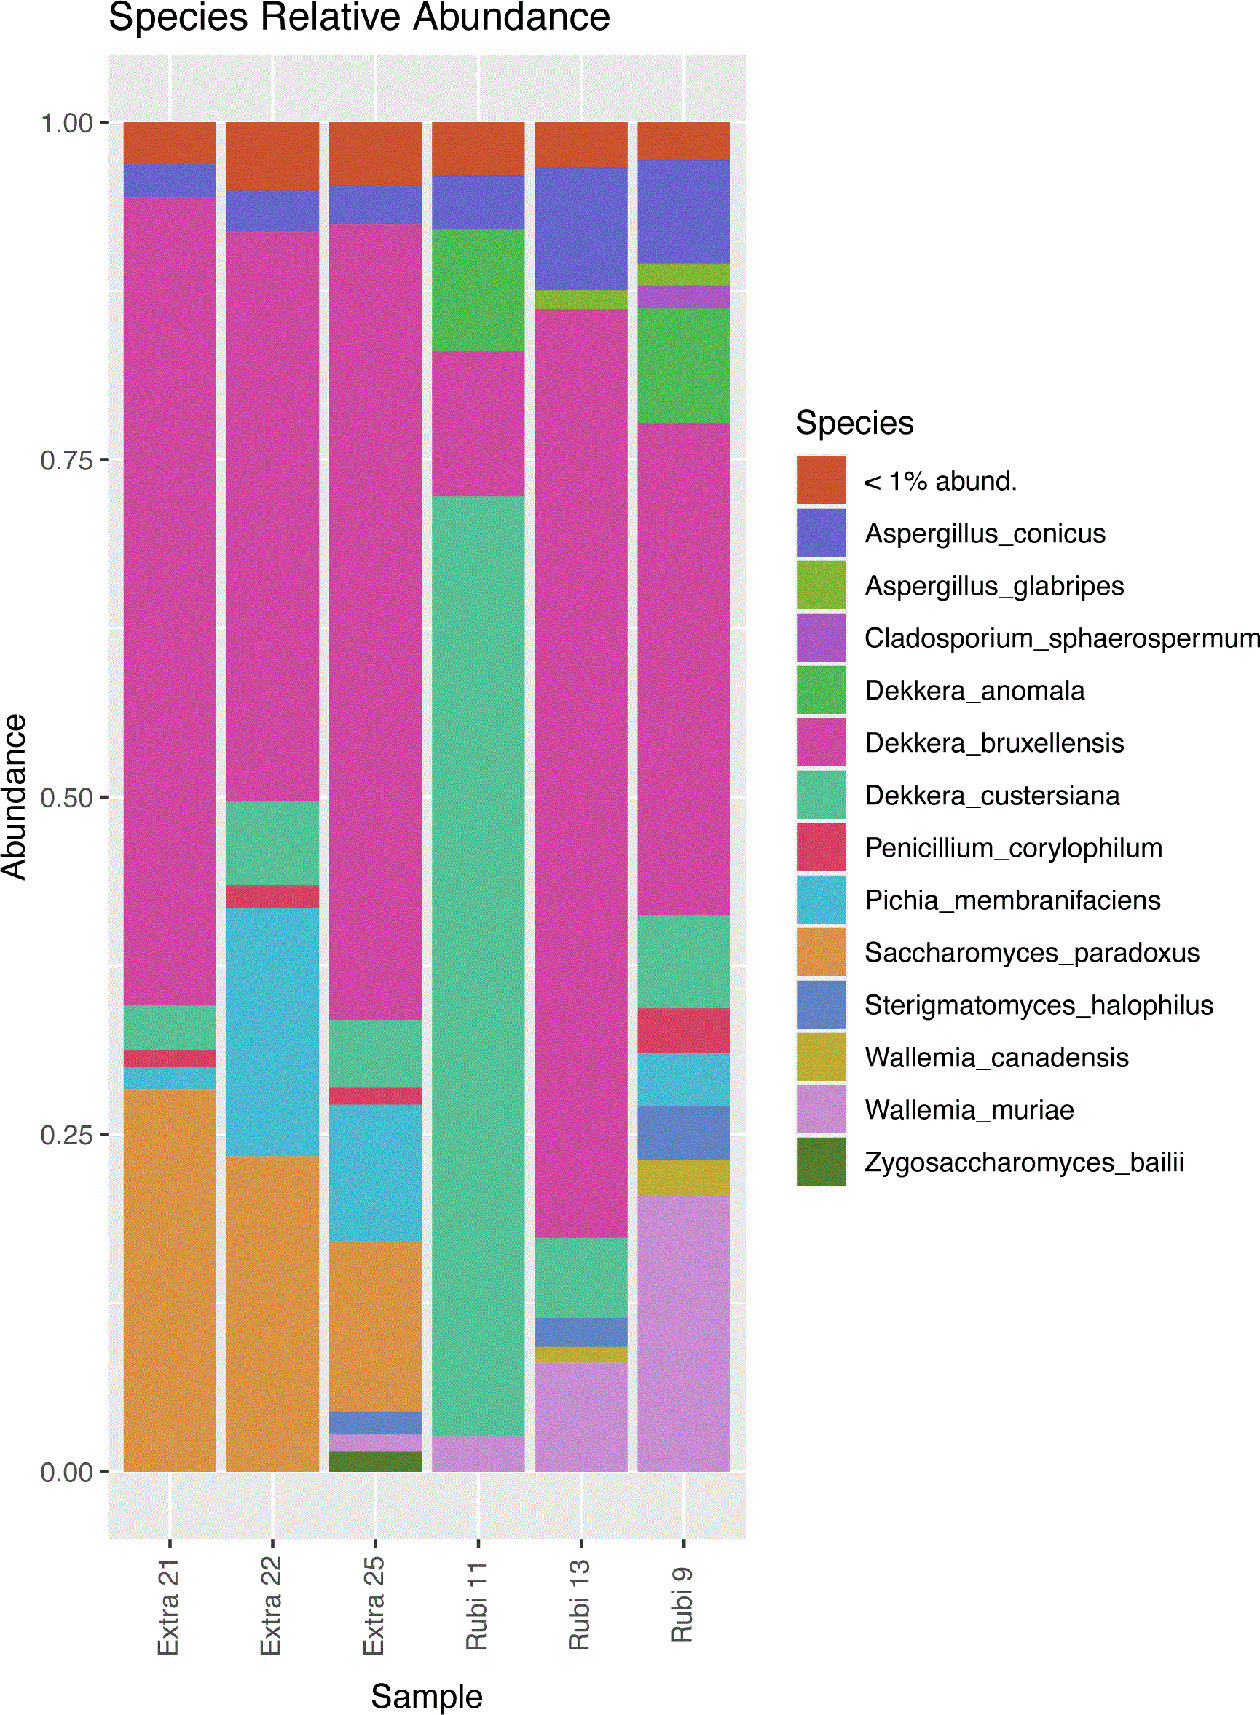
\includegraphics[width=\textwidth]{images/orginal_doppelbock_relative_abundence.jpg}
        \caption{Original results}
    \end{subfigure}
    \hfill
    \begin{subfigure}[b]{0.45\textwidth}
        \centering
        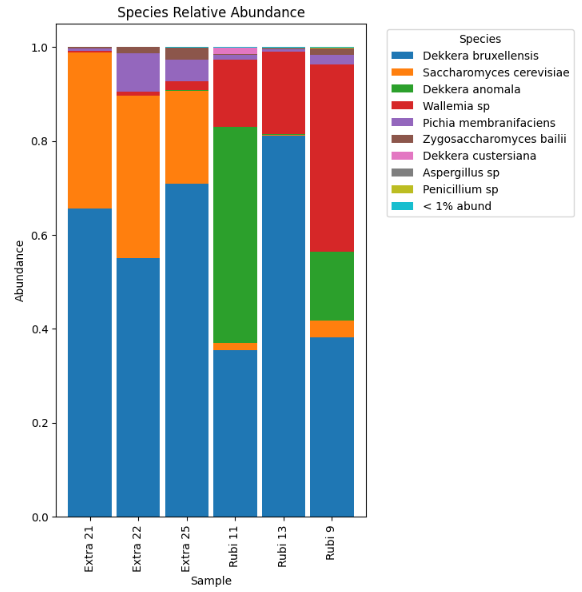
\includegraphics[width=\textwidth]{images/doppelbock_relative_abundence.png}
        \caption{Reproduced results}
    \end{subfigure}
    \caption{Fungal species relative abundance}
    \small The relative abundance of fungal taxa at the species level across various beer styles is depicted. Notably, \textit{Dekkera} stands out as the most abundant genus in both beer styles examined.
    \label{fig:methods:doppelbock_relative_abundence_fungal}
\end{figure}

    In addition to the presence of \textit{Pichia}, the Original results showed the detection of \textit{Aspergillus} and \textit{Penicillium}. Notably, \textit{Hanseniaspora uvarum}, a yeast commonly found on grapes\cite{fleet1993wine}, was also identified, indicating its presence in the samples.

    
\begin{table}[H]
\centering
\begin{threeparttable}
\caption{Comparison of Original and reproduced estimates and T-test results}
\begin{tabular}{c}
\begin{subtable}{\textwidth}
\centering
\caption{Species richness and diversity of fungal communities in Extra and Rubi beer barrels}
\begin{tabular}{|c|c|c|c|c|c|c|}
\hline
\multirow{2}{*}{Sample} & \multicolumn{2}{c|}{Chao1} & \multicolumn{2}{c|}{Shannon} & \multicolumn{2}{c|}{Simpson} \\ \cline{2-7} 
                        & Original & Reproduced & Original & Reproduced & Original & Reproduced \\ \hline
Extra \#21              & 48    & 42  & 2.07    & 2.50    & 0.83    & 0.76    \\ \hline
Extra \#22              & 67.5  & 61  & 2.45    & 2.94    & 0.87    & 0.80    \\ \hline
Extra \#25              & 98.6  & 94  & 2.53    & 3.31    & 0.86    & 0.82    \\ \hline
Rubi \#11               & 70.5  & 65  & 1.88    & 3.46    & 0.72    & 0.82    \\ \hline
Rubi \#13               & 90.2  & 89  & 2.16    & 2.71    & 0.77    & 0.65    \\ \hline
Rubi \#9                & 117.2 & 104 & 3.14    & 4.16    & 0.92    & 0.89    \\ \hline
\end{tabular}
\end{subtable}
\\
\begin{subtable}{\textwidth}
\centering
\caption{T-test results for Original vs Reproduced estimates}
\begin{tabular}{|l|r|r|}
\hline
  Index &  T-statistic &  p-value \\
\hline
  Chao1 &    -3.238 & 0.0230 \\
\hline
Shannon &    -8.748 & 0.0003 \\
\hline
Simpson &     7.000 & 0.0009 \\
\hline
\end{tabular}
\end{subtable}
\end{tabular}
\begin{tablenotes}[flushleft]
\footnotesize
\item \textbf{Note:} Chao1 represents the Chao1 species richness estimator.
\item Shannon denotes the Shannon index of biodiversity. Higher values indicate higher diversity.
\item Simpson represents the Simpson diversity index. Values range from 0 (simplest) to 1 (most diverse).
\end{tablenotes}
\end{threeparttable}
\label{tab:combined_table}
\end{table}

Upon reviewing the results from the original study and the reproduced results of diversity indices for the beer samples on the diversity of fungal communities, several notable points of comparison and contrast emerge.

First, looking at the Chao1 biodiversity index, the reproduced results indicate generally lower estimates across all samples, with a noticeable decrease in Rubi \#9 (from 117.2 to 104) and Extra \#21 (from 48 to 42). Chao1 is a non-parametric estimator used to predict the true species richness of a community, and thus these lower estimates suggest that the reproduced results predict fewer unique species in each sample than the original study.

In contrast, the Shannon index, which measures the entropy (or unpredictability) of species diversity within a community, is consistently higher in the reproduced results across all samples. This suggests that the reproduced results found a greater degree of diversity, possibly with more evenly distributed species within each sample. The most pronounced differences can be observed in Rubi \#11 (from 1.88 to 3.46) and Extra \#22 (from 2.45 to 2.94).

Similarly, the Simpson index, which is a measure of species diversity that gives more weight to the abundant species, also shows an increase in all but one sample (Rubi \#13, where it decreased from 0.77 to 0.65) in the reproduced results. This suggests an increased evenness and diversity, as a higher Simpson's index implies that individuals are distributed more evenly among species.

In summary, with these differences in individual measures and t-test results, the data suggests that the reproduced results have more evenly distributed diversity but less richness.

    \paragraph*{Bacterial diversity}

In our reanalysis of the bacterial communities present in two distinct styles of beer, we found the overall bacterial distribution to be consistent with the original study (Figure \ref{fig:methods:doppelbock_relative_abundence_bacterial}). The primary microbial constituents encompassed just three genera, each with a relative abundance of 1\% or more. These pivotal genera were identified as \textit{Pediococcus}, \textit{Lactobacillus}, and \textit{Acetobacter}.

\begin{figure}[H]
     \centering
     \begin{subfigure}[b]{0.45\textwidth}
         \centering
         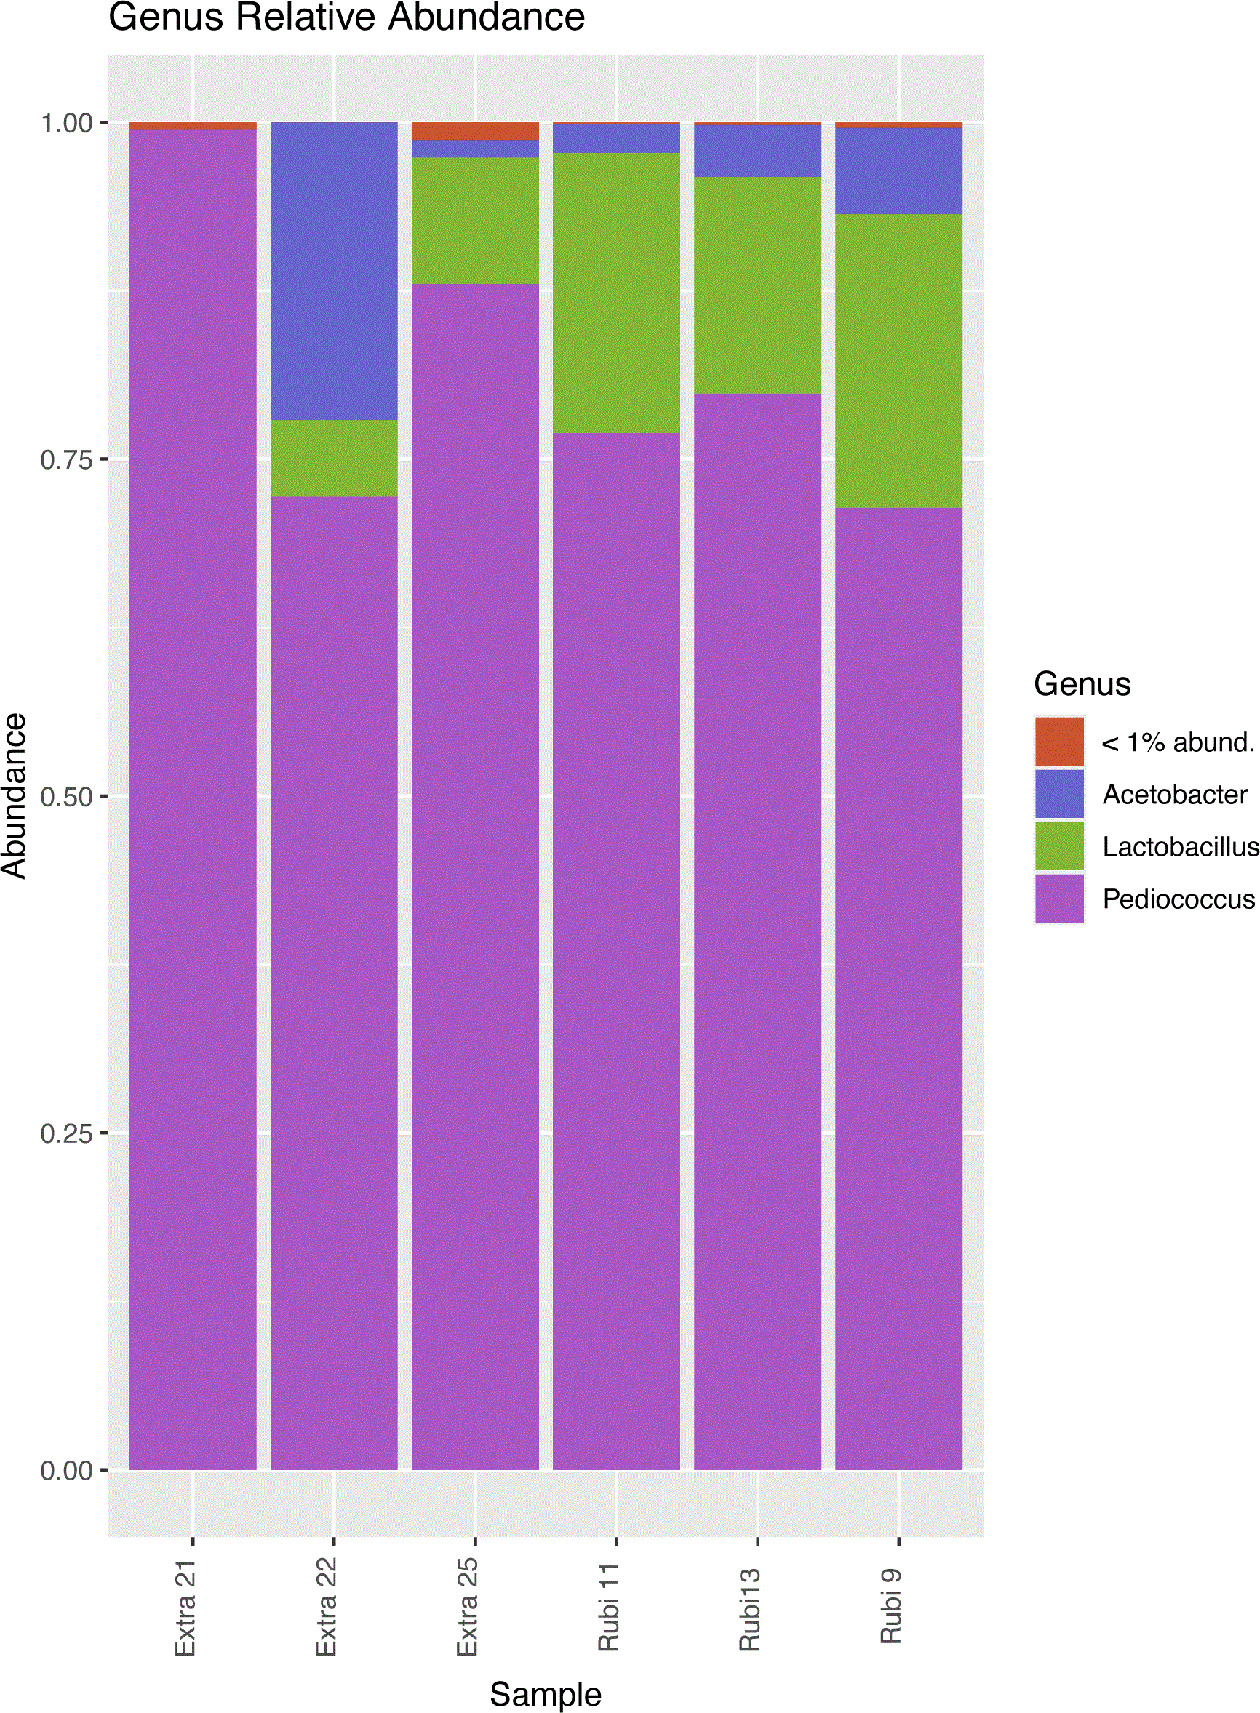
\includegraphics[width=\textwidth]{images/original_doppel_baceteria_genus_relative_abundance.jpg}
        \caption{Original results}
     \end{subfigure}
     \hfill
     \begin{subfigure}[b]{0.45\textwidth}
         \centering
         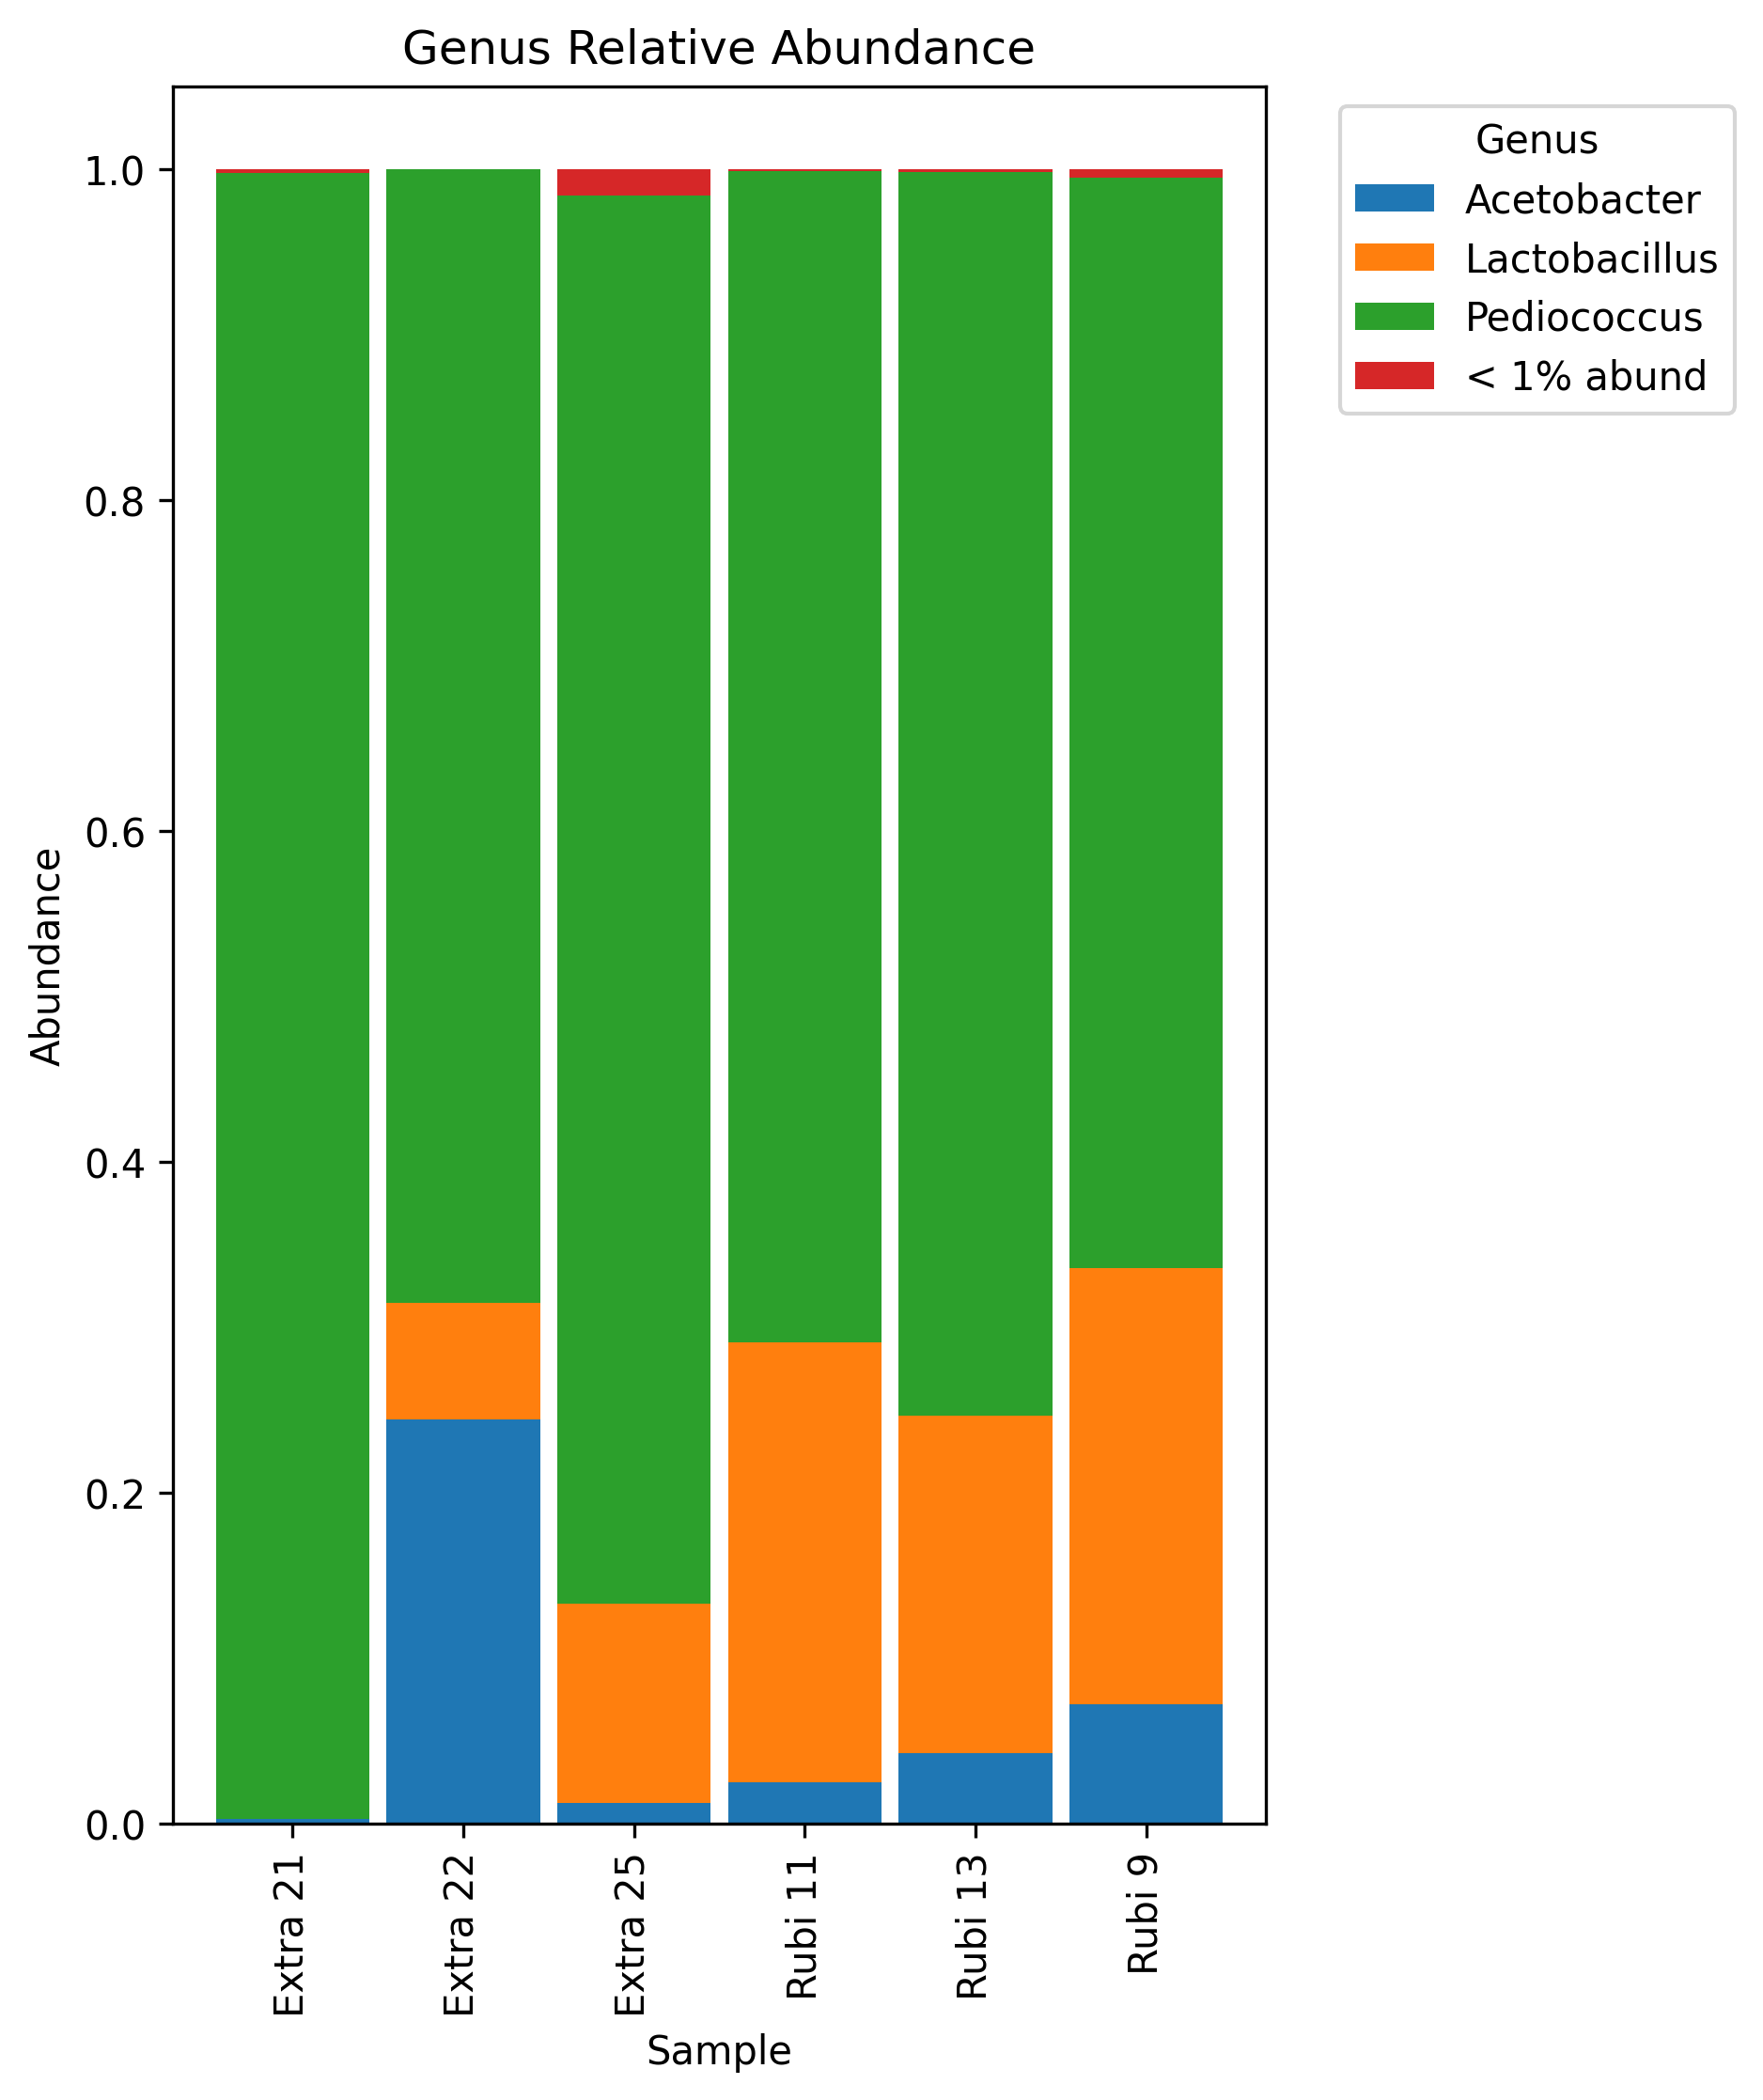
\includegraphics[width=\textwidth]{images/doppel_baceteria_genus_relative_abundance.png}
        \caption{Reproduced results}
     \end{subfigure}
    \caption{Bacterial genus relative abundance}
    \small Regarding the relative abundance of bacterial taxa at the genus level within the beer styles, the produced results align well with the findings of the original study.
    \label{fig:methods:doppelbock_relative_abundence_bacterial}
\end{figure}

Discrepancies in the prevalence of these bacterial genera were more pronounced in the samples of Extra beer when compared to the Ruby variant. A stark example was found in Extra barrel \#21 where \textit{Pediococcus} appeared to be the predominant microorganism, accounting for a staggering 99\% of the bacterial population. Conversely, Extra barrel \#22 was characterized by the highest percentage of \textit{Acetobacter} across all beer samples, recorded at 22\%. Extra barrel \#25 was notable for exhibiting the greatest abundance of \textit{Lactobacillus} among the Extra samples. Interestingly, this marked variability was not reflected in the Ruby beer samples. Instead, we observed a much more uniform distribution of bacterial genera across the Ruby barrels.


\begin{table}[h!]
\centering
\begin{threeparttable}
\caption{Comparison of Original and reproduced estimates and T-test results}
\begin{tabular}{c}
\begin{subtable}{\textwidth}
\centering
\caption{Species richness and diversity of bacterial communities in Extra and Rubi beer barrels}
\begin{tabular}{|c|c|c|c|c|c|c|}
\hline
\multirow{2}{*}{Sample} & \multicolumn{2}{c|}{Chao1} & \multicolumn{2}{c|}{Shannon} & \multicolumn{2}{c|}{Simpson} \\ \cline{2-7} 
                        & Original & Reproduced & Original & Reproduced & Original & Reproduced \\ \hline
Extra \#21              & 10   & 13  & 1.45    & 1.73    & 0.74    & 0.66    \\ \hline
Extra \#22              & 10   & 13  & 1.86    & 2.45    & 0.82    & 0.78    \\ \hline
Extra \#25              & 18   & 31  & 1.88    & 2.57    & 0.81    & 0.77    \\ \hline
Rubi \#11               & 9    & 19  & 1.72    & 2.27    & 0.80    & 0.76    \\ \hline
Rubi \#13               & 17   & 24  & 1.96    & 2.69    & 0.83    & 0.79    \\ \hline
Rubi \#9                & 10   & 11  & 1.75    & 2.30    & 0.81    & 0.77    \\ \hline
\end{tabular}
\end{subtable}
\\
\begin{subtable}{1\textwidth}
\centering
\caption{T-test results for Original vs reproduced estimates}
\begin{tabular}{|l|r|r|}
\hline
  Index &  T-statistic &  p-value \\
\hline
  Chao1 &     3.845 & 0.012 \\
\hline
Shannon &    -4.537 & 0.006 \\
\hline
Simpson &     1.257 & 0.264 \\
\hline
\end{tabular}
\end{subtable}
\end{tabular}
\begin{tablenotes}[flushleft]
\footnotesize
\item \textbf{Note:} Chao1 represents the Chao1 species richness estimator.
\item Shannon denotes the Shannon index of biodiversity. Higher values indicate higher diversity.
\item Simpson represents the Simpson diversity index. Values range from 0 (simplest) to 1 (most diverse).
\end{tablenotes}
\end{threeparttable}
\label{tab:combined_table}
\end{table}


The Chao1 index, an estimator of species richness, appears to show higher values in the reproduced results than in the original, for all samples. The increase in Chao1 values implies that the re-analysis might have identified more species within the samples. A T-test comparing the original and reproduced Chao1 values reveals a significant difference with a p-value of 0.012. This indicates that the difference in species richness estimates between the original and reproduced data is not likely due to chance.

For the Shannon index, which incorporates both species richness and evenness, the reproduced results also display higher values for all samples. The T-test further corroborates this observation with a statistically significant p-value of 0.006. Higher Shannon values suggest that the bacterial communities identified in the re-analysis are not only richer in species but also display a more even distribution among the identified species.

In contrast, the Simpson index, which places greater weight on dominant species, reveals no statistically significant difference between the original and reproduced estimates (p-value = 0.264). This suggests that, despite variations in species richness and evenness, the overall dominance structure of the bacterial communities remains relatively consistent between the original and reproduced results.

In summary, the comparison between the original and reproduced diversity estimates reveals a significant difference in the Chao1 and Shannon indices, but not in the Simpson index. This suggests that while species richness and evenness may be affected by the improved workflow, the overall dominance structure of the communities remains stable across studies.

% The two sets of diversity indices on bacterial diversity, one from the original study and the other from the Reproduction offer interesting insights into the bacterial diversity within the beer samples.

% The Chao1 index, a measure of species richness, is higher in all samples in the reproduced results compared to the original study. This indicates that the reproduced results predict a greater number of unique bacterial species in each beer sample. The most remarkable change can be seen in Extra \#25, where the Chao1 index increased from 18 to 31.

% The Shannon index, which encapsulates both species richness and evenness, is also consistently higher in the reproduced results. This suggests that, according to the reproduced results, each beer sample harbors a more diverse and evenly distributed bacterial community. For instance, the Shannon index in Rubi \#13 increased from 1.96 in the original study to 2.69 in the reproduced results.

% The Simpson index, a measure more sensitive to dominant species, is slightly lower in the reproduced results for most samples, suggesting an increased evenness among bacterial species. The most evident decrease is seen in Extra \#21, where the Simpson index fell from 0.74 to 0.66.

% Despite these changes, both analyses align in their main conclusion: the ANOVA results indicate no significant effect of beer style on bacterial diversity.

\subsection{BeerMicroDB overview}

    \begin{figure}[H]
        \centering
        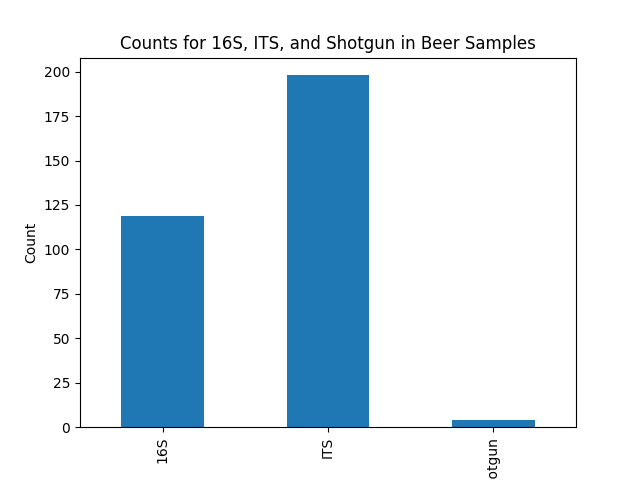
\includegraphics[scale=0.5]{images/overview/16S_ITS_Shotgun.png}
        \caption{Beer sample count}
        \label{fig:results:beer_sample_count}
    \end{figure}

    Overall, the BeerMicroDB database comprises a total of 119 samples analyzed via 16S rRNA gene sequencing, 198 samples examined using ITS sequencing, and a significantly smaller subset of just 4 samples studied using shotgun metagenomic sequencing (Figure \ref{fig:results:beer_sample_count}). It's clear that our current database is predominantly populated with data from metabarcoding methods, namely 16S and ITS sequencing.
    
    Despite the robustness and insights these methods offer, the relative scarcity of shotgun metagenomic data in our collection does present a limitation in terms of the depth and granularity of our microbial community analysis. We acknowledge this disparity in data types and emphasize the need to enhance the proportion of shotgun metagenomic data within BeerMicroDB. As such, we are hopeful that with the recommencement of the BeerDEcoded and Street Science Project, which help public citizens aware of bioinformatics by learning from sequencing to analyzing beer microbiome, we will be able to enrich our database with more shotgun metagenomic data, thus improving the breadth and depth of our analyses and leading to more nuanced insights into the beer microbiome.

\subsubsection{Fungal microbiome overview}

This section gives an overview of fungal microbiome results.

As shown in figure \ref{fig:methods:top10_beer_fungal}, the beer sample with the highest fungal species count was "Sesotho," which contained an impressive number of 70 distinct species. This was followed by "Rubi Marzen Lager" and "Extra Doppelbock Lager," hosting 51 and 46 species respectively. These beers exhibited significantly higher fungal biodiversity compared to others in the analysis. For instance, "Blond Beer (8.88\%)," "Chimay Red Cap," "Waldbier 2014 Wienerwald," "La Fourbe," "Valaisanne Amrich," and "La Montheysanne" exhibited species counts ranging from 7 to 21.

    \begin{figure}[H]
        \centering
        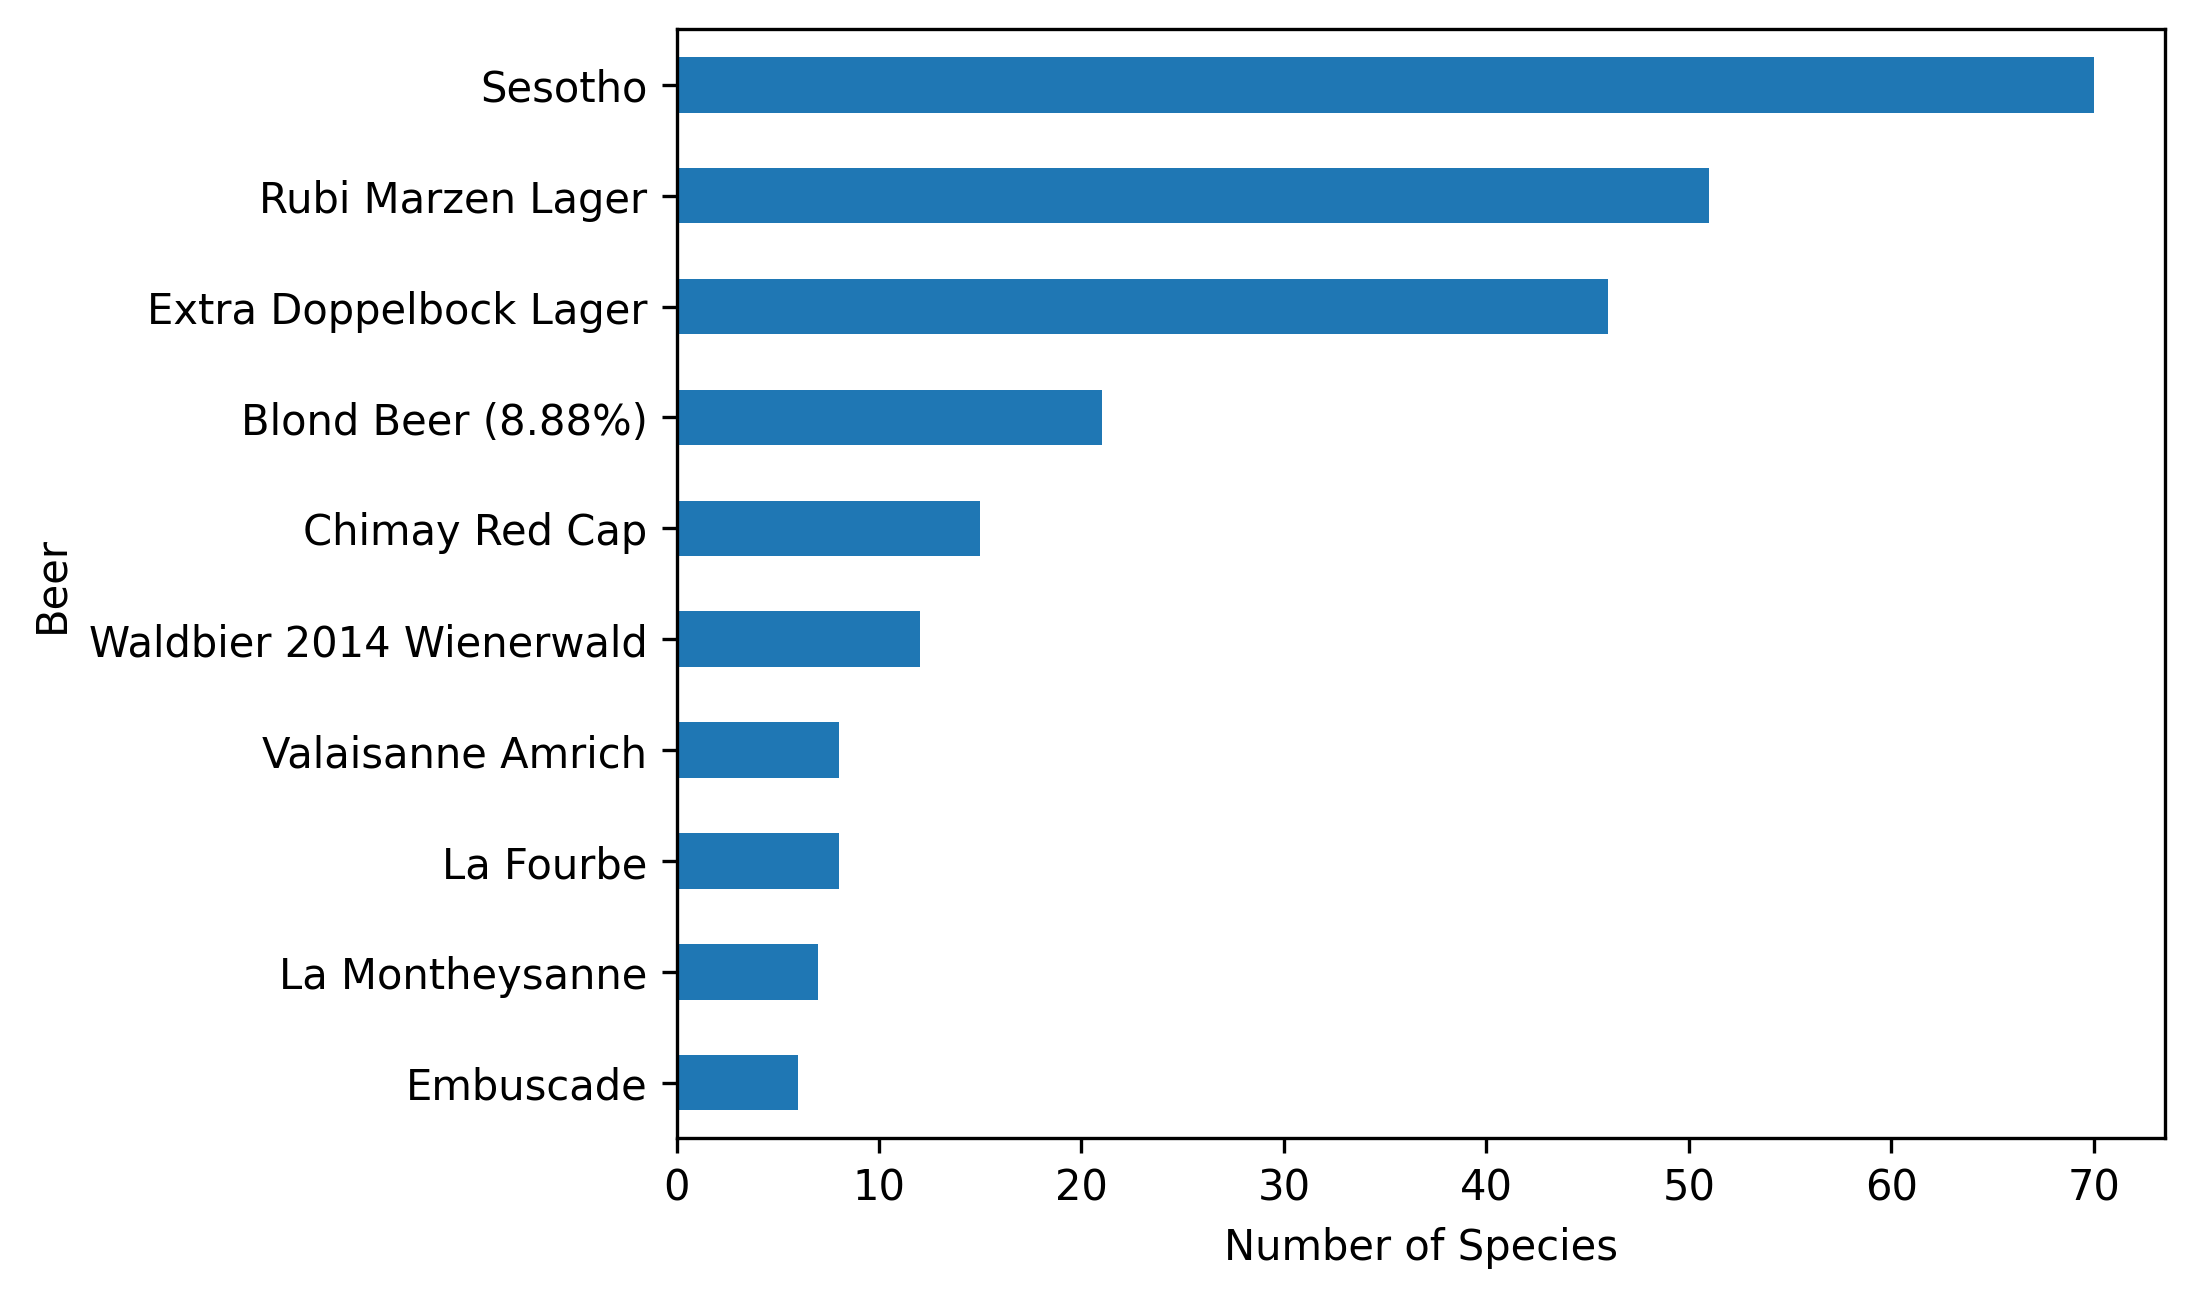
\includegraphics[scale=0.7]{images/overview/top10_beers_fungal.png}
        \caption{Top 10 Beers with the Highest Species Count}
        \small Among all beer types, Sesotho, which undergoes spontaneous fermentation, exhibits the highest count of fungal species.
        \label{fig:methods:top10_beer_fungal}
    \end{figure}
    
The data suggest that beer type and presumably the specific brewing process might significantly influence the diversity of fungal species in the final product. The top beers all have less regulated brewing processes and conditions.

The fungal species with the highest frequency of occurrence across the beer samples was \textit{Saccharomyces cerevisiae} identified in 126 instances (Figure \ref{fig:results:top10_species_fungal}). This is unsurprising, given that \textit{S. cerevisiae} is a commonly used yeast in the brewing industry due to its robust fermentation capabilities and its contribution to beer's distinctive flavor profiles.

    \begin{figure}[H]
        \centering
        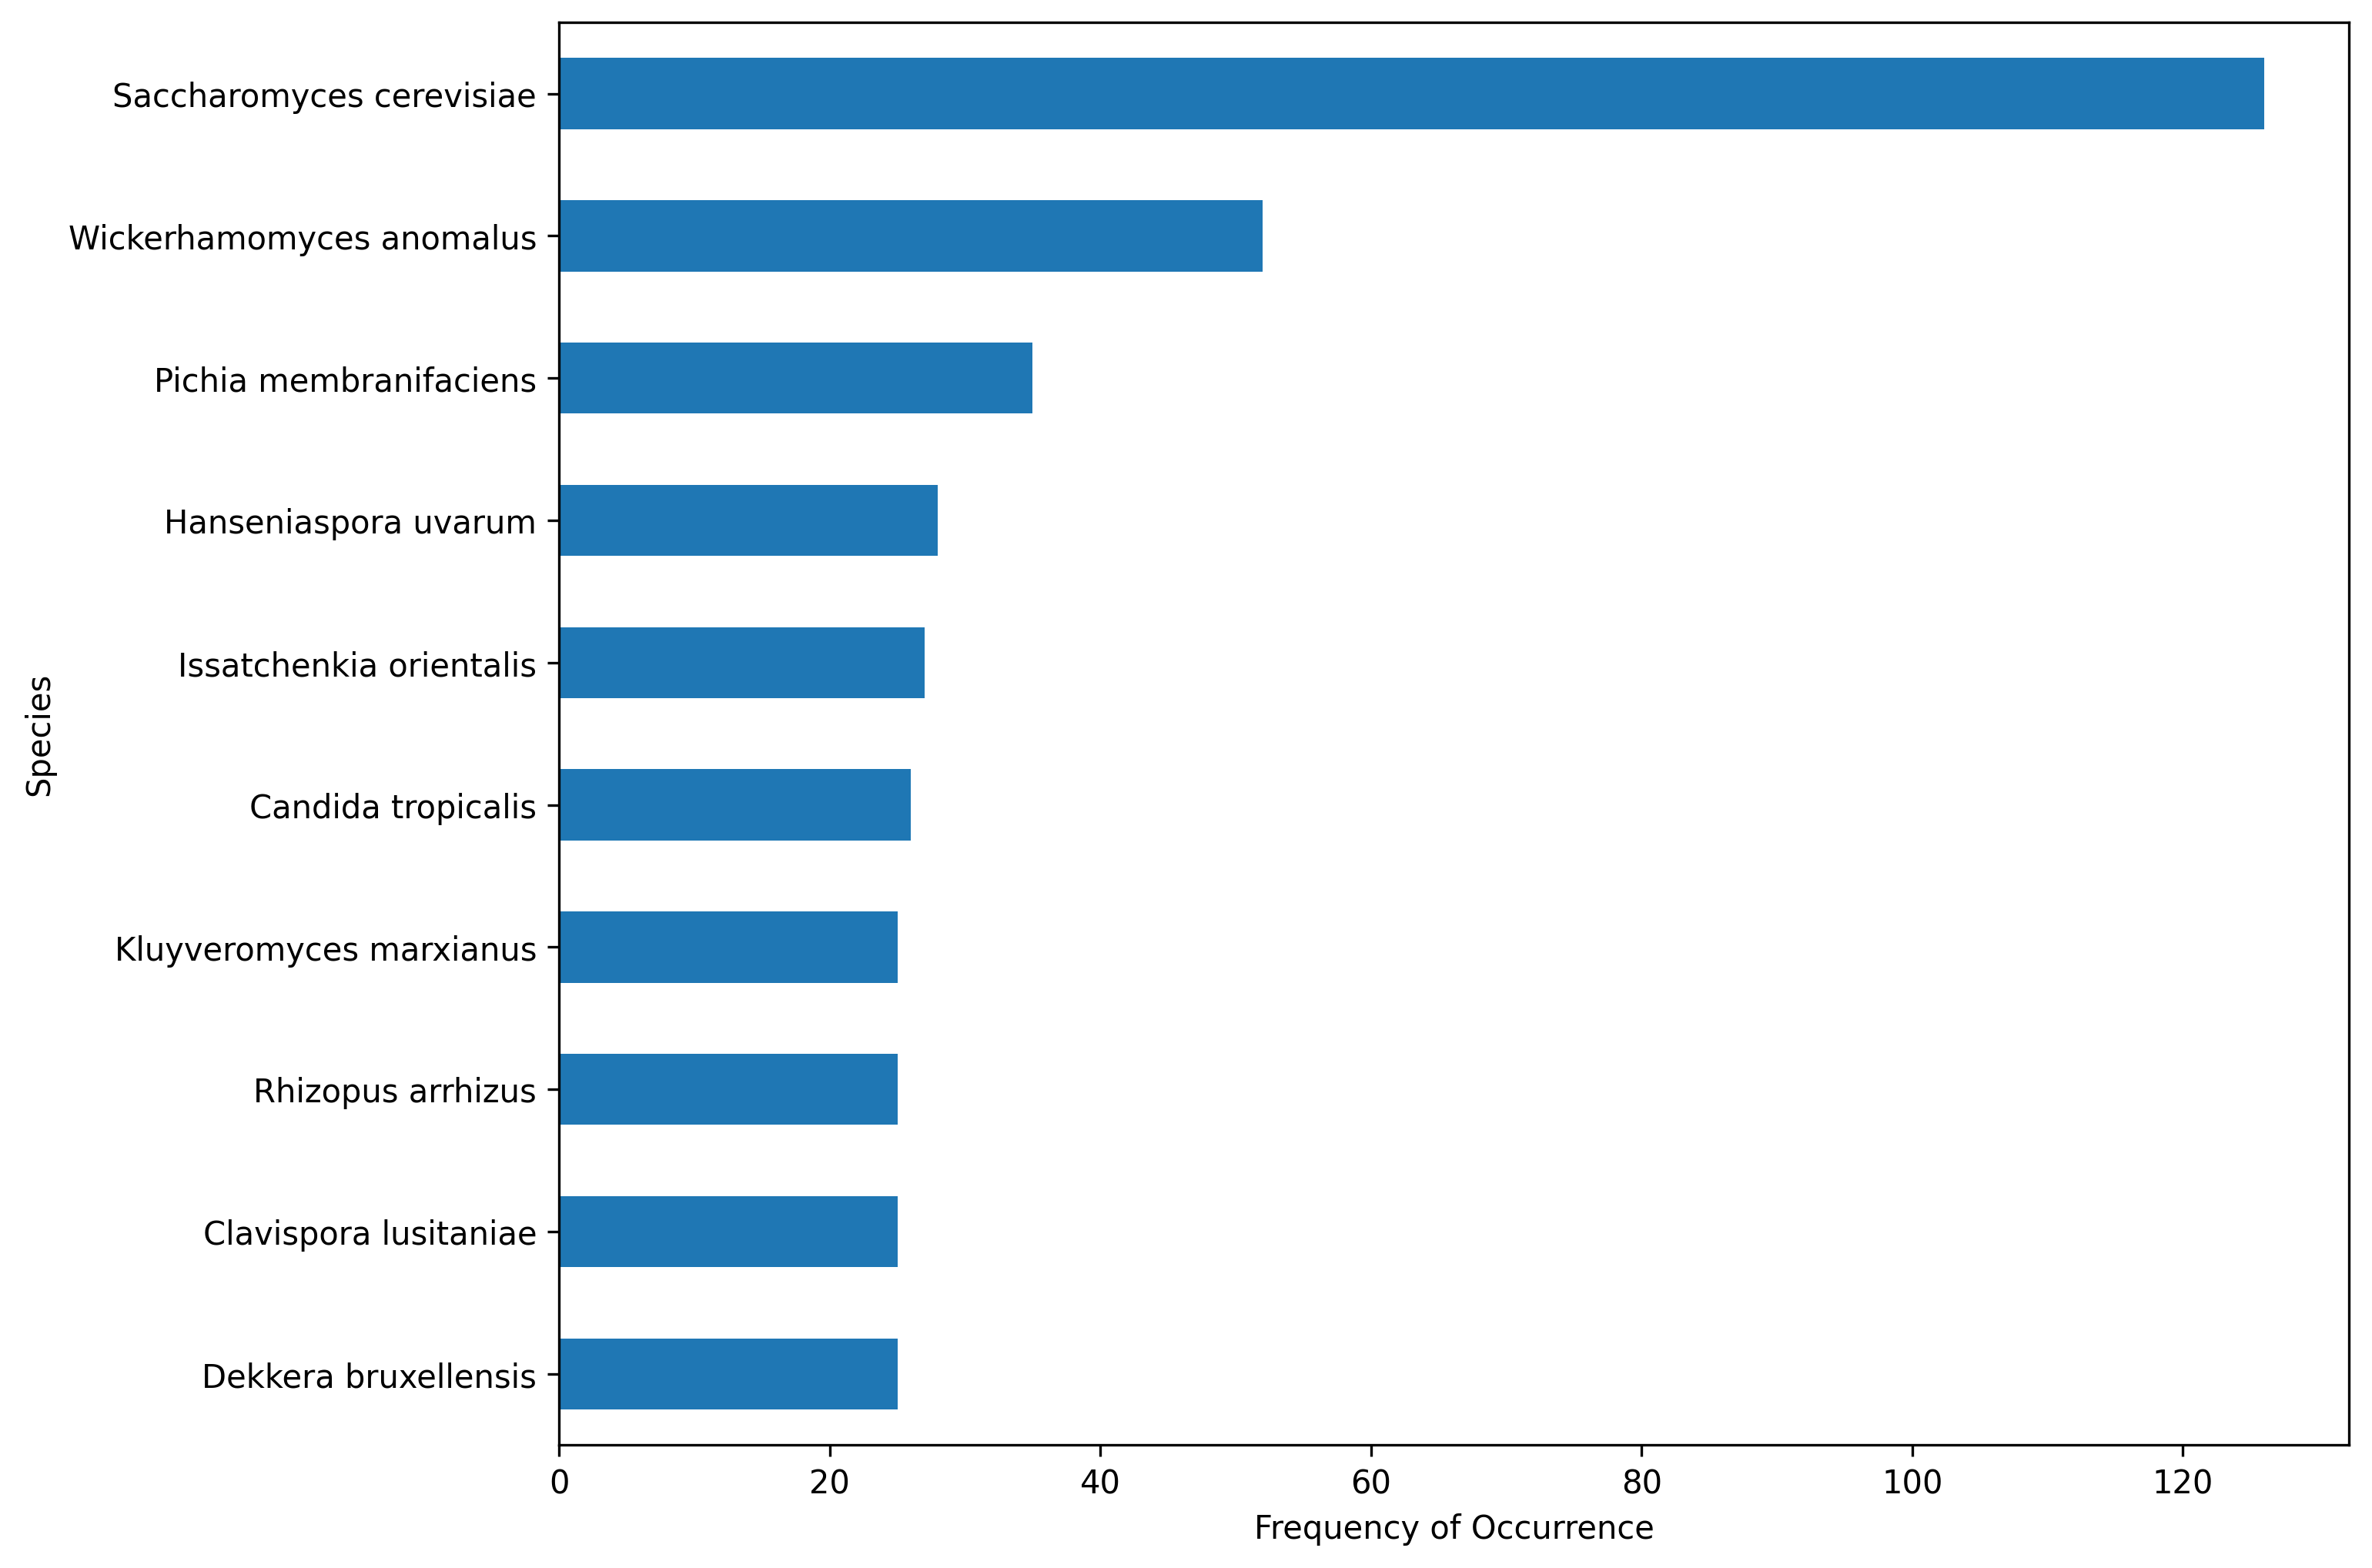
\includegraphics[scale=0.5]{images/overview/top10_species_fungal.png}
        \caption{Top 10 Species with the Highest Frequency of Occurrence}
        \small \textit{Saccharomyces cerevisiae} unequivocally emerges as the most prevalent species. It is closely followed by \textit{Wickerhamomyces anomalus}, which holds a slight advantage over other fungal species in the dataset.
        \label{fig:results:top10_species_fungal}
    \end{figure}
    
Other recurrent species include \textit{Wickerhamomyces anomalus} and \textit{Pichia membranifaciens} noted in 52 and 35 instances respectively, and a group of species including \textit{Hanseniaspora uvarum}, \textit{Issatchenkia orientalis}, \textit{Candida tropicalis}, \textit{Dekkera bruxellensis}, \textit{Clavispora lusitaniae}, \textit{Rhizopus arrhizus} and \textit{Kluyveromyces marxianus} each of which appeared 25-28 times.

These findings highlight the prevalence and importance of these species in the beer brewing ecosystem. It should be noted that while some of these species, such as \textit{D. bruxellensis} can potentially impart off-flavors to beer, others like \textit{K. marxianus} and \textit{W. anomalus} are known to have potentially beneficial effects on flavor and aroma complexity as shown before. Therefore, these species' presence and frequency could play a significant role in shaping the unique characteristics of the beers analyzed.
        


\subsubsection{Bacterial microbiome overview}

This section gives an overview of bacterial microbiome results from the 119 16S samples. The data revealed a diverse range of bacterial species associated with the beers, indicating the presence of complex microbial communities that potentially contribute to the unique flavors and characteristics of each brew. Two key aspects were explored: the top 10 beers with the highest species count and the top 10 species with the highest frequency of occurrence.

    \begin{figure}[H]
        \centering
        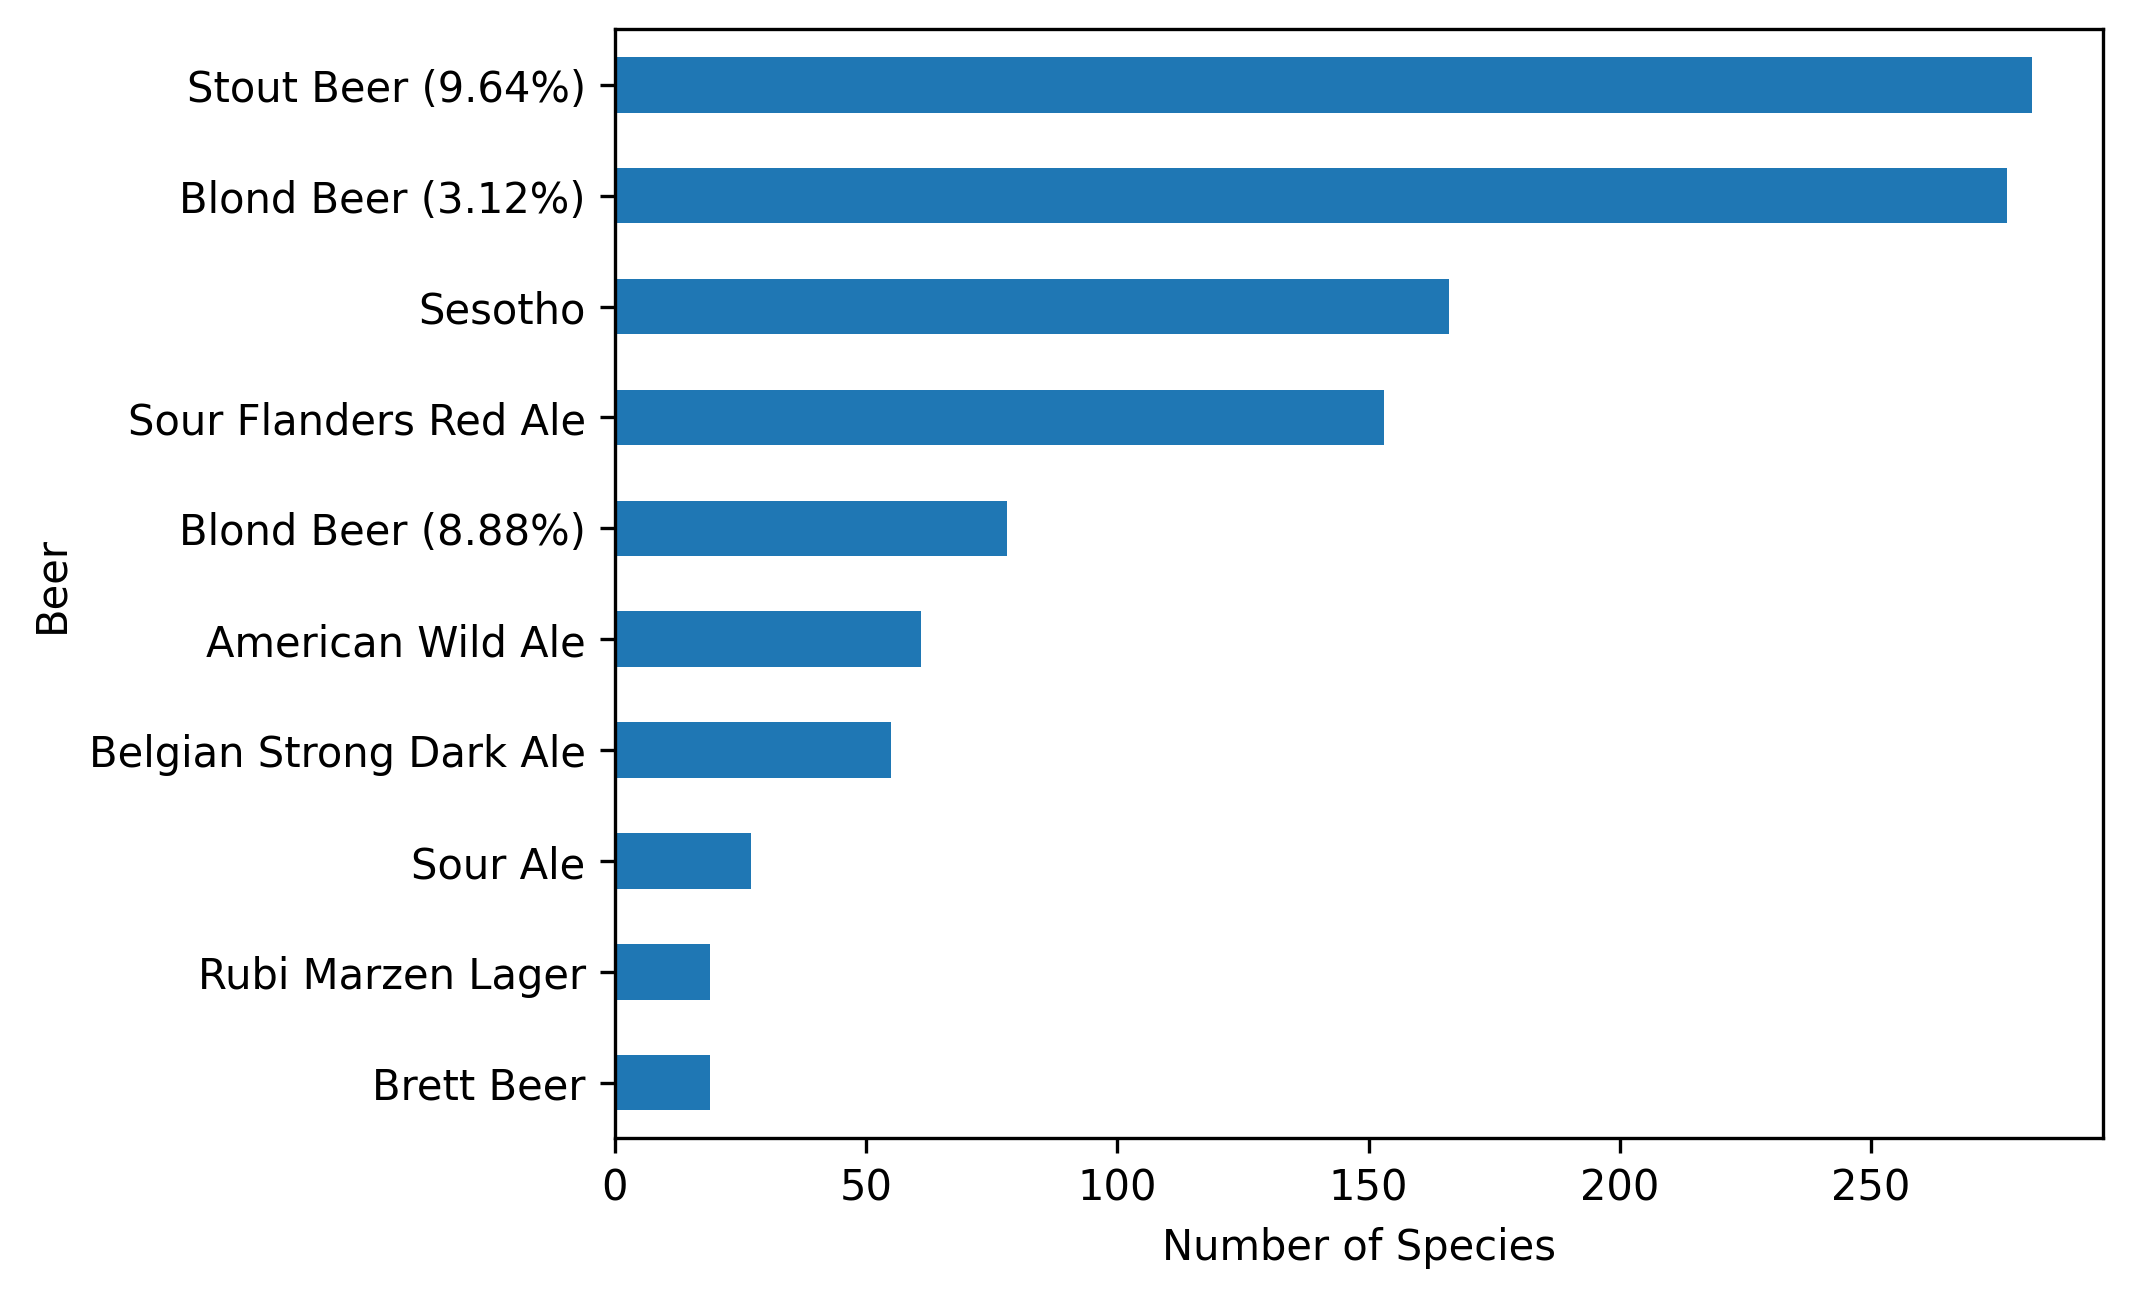
\includegraphics[scale=0.7]{images/overview/top10_beers_bac.png}
        \caption{Top 10 Beers with the Highest Species Count}
        \small The stout beer (9.64\%) and blond beer (3.12\%) lead in terms of bacterial species richness. They are closely followed by Sesotho and sour Flanders red ale in the subsequent rankings.
        \label{fig:results:top10_beer_bacterial}
    \end{figure}

The analysis of the bacterial microbiome in different types of beer unveils a complex and diverse bacterial composition. Notably, Stout Beer with a 9.64\% alcohol content exhibits the highest species count (282), followed closely by Blond Beer at two different alcohol percentages, 3.12\% (277 species) and 8.88\% (78 species) shown in the figure \ref{fig:results:top10_beer_bacterial}.

Interestingly, the presence of a beer called Sesotho, containing 166 species, indicates a potential regional influence on microbial diversity. Other notable inclusions are Sour Flanders Red Ale (153 species), American Wild Ale (61 species), Belgian Strong Dark Ale (55 species), Sour Ale (27 species), Brett Beer (19 species), and Rubi Marzen Lager (19 species).

The stour beer and blond beer went through a barrel aging process, this could be the reason why they have a high bacterial species count. And Sesotho which is spontaneously fermented in the wild environment, could be the reason why it is with high diversities. Overall, as we can see, the sour beer, ale has higher bacterial diversity.

    \begin{figure}[H]
        \centering
        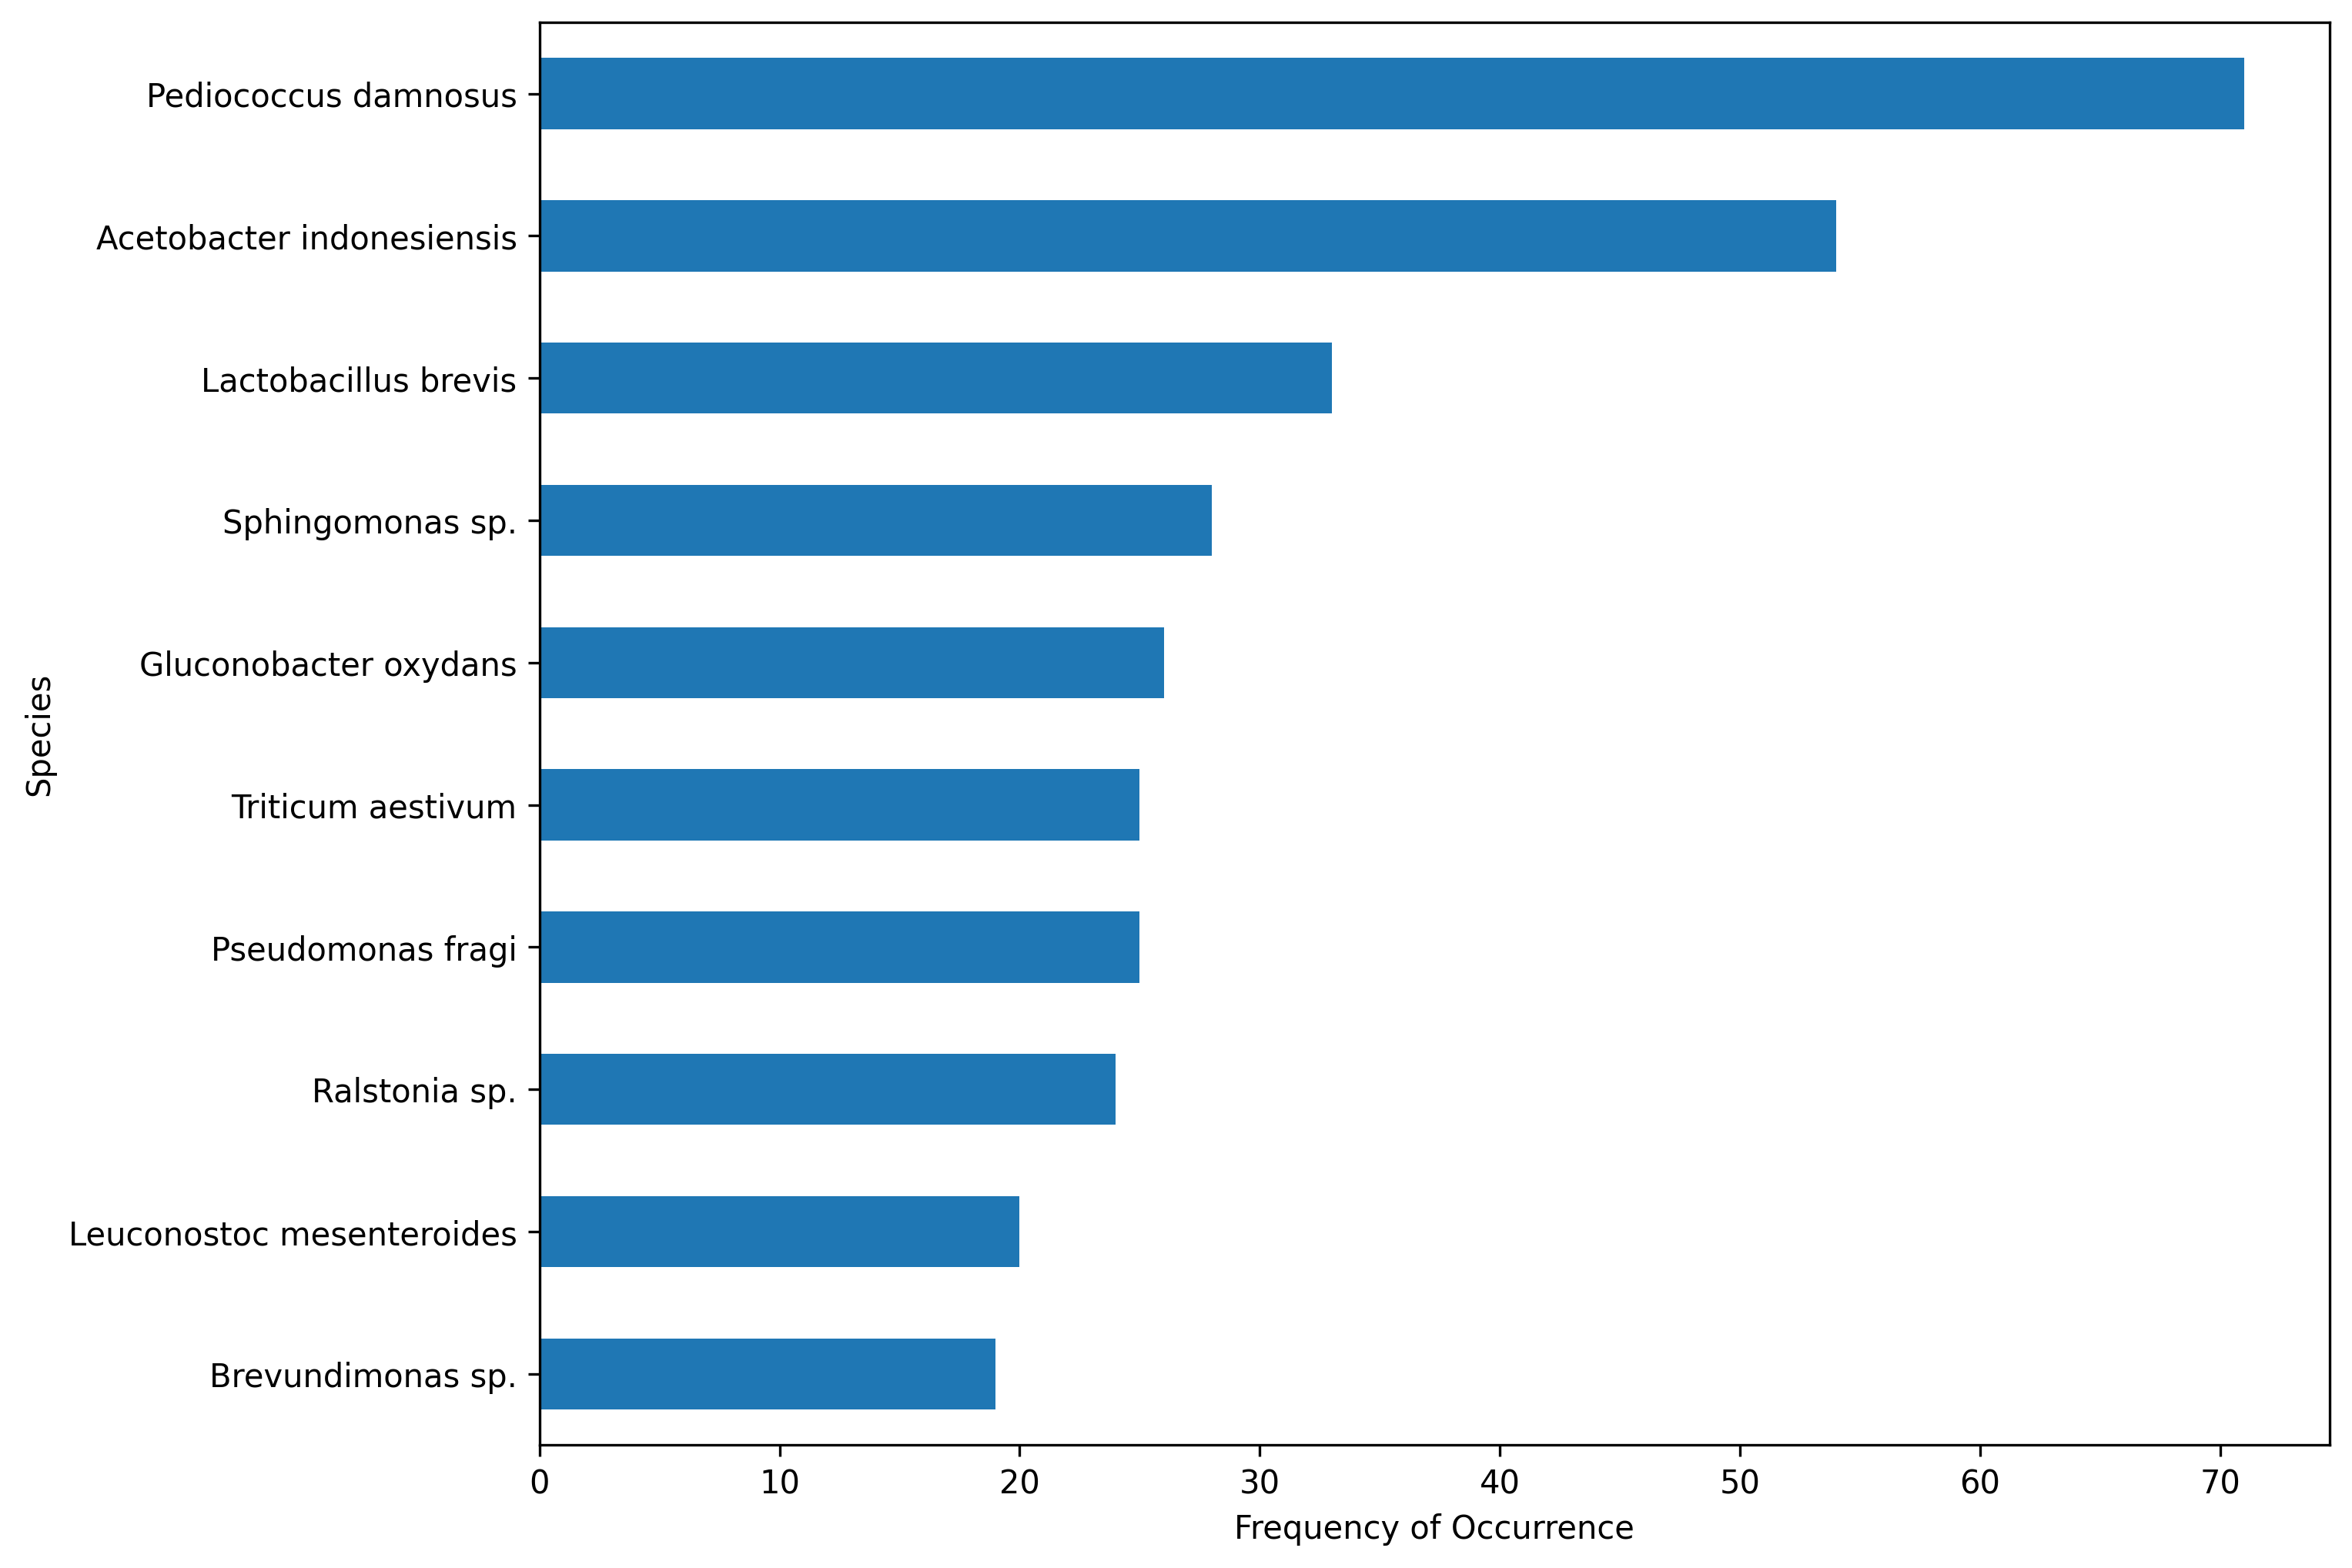
\includegraphics[scale=0.5]{images/overview/top10_species_bac.png}
        \caption{Top 10 Species with the Highest Frequency of Occurrence}
        \small The species \textit{Pediococcus damnosus} emerged as the most dominant, closely followed by \textit{Acetobacter indonesiensis}. Among the subsequent species observed, eight exhibited fewer differences in their frequency of occurrence.
        \label{fig:methods:top10_species_bac}
    \end{figure}
    
A close inspection of the top ten bacterial species, in terms of frequency of occurrence, highlights the significant presence of certain bacteria across different beer samples (Figure \ref{fig:methods:top10_species_bac}). The most prevalent species is \textit{Pediococcus damnosus}, found in 71 samples, followed by \textit{Acetobacter indonesiensis} (54), \textit{Lactobacillus brevis} (33), and \textit{Sphingomonas sp.} (28).

The presence of \textit{Gluconobacter oxydans} (26), \textit{Pseudomonas fragi} (25), \textit{Triticum aestivum} (25), \textit{Ralstonia sp.} (24), \textit{Leuconostoc mesenteroides} (20), and \textit{Brevundimonas sp.} (19) also suggests their common role in various beer types. These species are often involved in fermentation processes and may contribute to the unique flavors, aromas, and characteristics of the beer.

Furthermore, the occurrence of \textit{Triticum aestivum} might be indicative of wheat's role in certain beer formulations. The identification and characterization of these bacteria not only provide insights into the microbiological profile of different beers but also raise potential considerations in quality control, flavor development, and potential health aspects.

In conclusion, these findings serve as an essential resource for understanding the intricate bacterial ecology within various beer types, contributing to ongoing research in brewing science, quality assurance, and sensory analysis. Further studies may elucidate the specific roles and interactions of these microbial communities in shaping the attributes of the diverse world of beer.
     
% \section{Discussion}

\section{Conclusion}

    \begin{figure}[H]
        \centering
        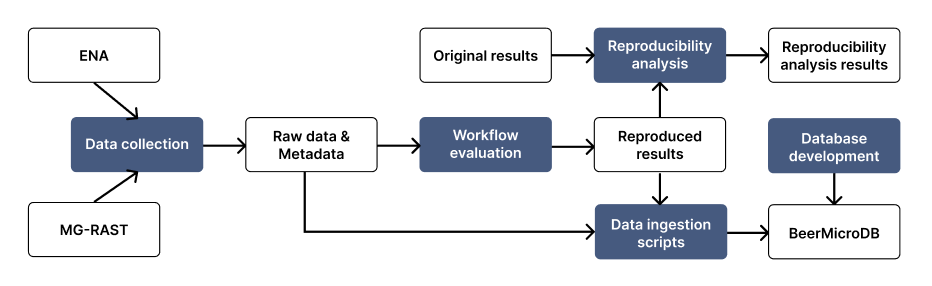
\includegraphics[scale=0.5]{images/overview.png}
        \caption{Thesis overview}
        \small In the overview of the thesis, the white box stands for the data and results, and the blue box symbolizes the action taken. The research starts with data collection, advancing to the evaluation of workflows, followed by an in-depth reproducibility analysis, and culminating in the construction of the BeerMicroDB.
        \label{fig:conclusion:overview}
    \end{figure}

    The thesis commences with the gathering of raw data and metadata from two sources: ENA and MG-RAST. Subsequently, two distinct workflows are employed: a metabarcoding workflow developed using \tool{QIIME 2} and a shotgun workflow facilitated by \tool{Kraken 2}. Both workflows have been implemented on the \tool{Galaxy} platform and automated through the Galaxy API Python library, known as \tool{BioBlend}. For the comparison of reproduced results with original findings, \tool{Jupyter Notebook} combined with \tool{Python} libraries such as \tool{Pandas}, \tool{Matplotlib}, and \tool{Seaborn} was utilized to undertake the reproducibility analysis. Based on the raw data metadata and the reproduced results, BeerMicroDB was constructed, integrating \tool{Express.js} and \tool{MongoDB} for backend operations and \tool{React.js} for frontend development.
    
    Upon the execution of the workflows, while these workflows had some variances, their overarching outcomes were in harmonious alignment with the conclusions of prior studies that we have collected. One of the principal outcomes drawn from these workflows was the evident richness in microbiome diversity observed in certain beer types, particularly those subjected to spontaneous fermentation and aging procedures. The spontaneously fermented beers include sesotho - a traditional African beer, along with Extra Doppelbock Lager and Rubi Marzen Lager. Concurrently, the aging process was predominantly linked with beers such as Blond Beer and stout beer. Contrastingly, when these beers were measured against their industrial counterparts, the distinction was clear. The aforementioned beers showcased a significantly more diverse microbiome profile. This resonates with the idea that traditional and specific brewing methods can indeed have a pronounced impact on the microbial diversity of the final product.
    
    Within the beer samples, bacterial species such as \textit{Pediococcus damnosus}, \textit{Acetobacter indonesiensis}, and \textit{Lactobacillus brevis} were predominant. On the fungal front, the dominance was held by species like \textit{Saccharomyces cerevisiae}, \textit{Wickerhamomyces anomalus}, and \textit{Pichia membranifaciens}.
    
    Our initiative to create a specialized microbiome database, named BeerMicroDB, has accumulated metadata and microbiome compositions encompassing 56 distinct beers and a total of 301 samples that are publicly available for users to browse and have an insight into beers and beer microbiomes. However, the research encountered certain limitations. The number of shotgun datasets is disproportionate relative to the metabarcoding datasets. Additionally, the \tool{QIIME 2} tool on \tool{Galaxy} currently lacks support for manifest files for data importation, given the obscured nature of data pathways in the cloud environment to its users. It's also worth noting that the present iteration of BeerMicroDB is limited to read-only access. The in-depth analysis of content in the database provided by BeerMicroDB appears to be lacking.
    
    Anticipating future advancements, there exists a keen interest in expanding the dataset spectrum, both in terms of quantity and the variety of beer types represented. Introducing more advanced statistical methods, such as principal component analysis (PCA), and potentially harnessing machine learning techniques could offer valuable insights into distinguishing the core beer microbiome associated with varying beer types or regional beer variations. Moreover, an objective lies in refining BeerMicroDB by incorporating user authentication mechanisms. This would potentially facilitate user-driven contributions, enabling them to append additional datasets and share their microbiome analysis outcomes, thereby enriching the repository.
% \include{appendix}

%\cleardoublepage
\printbibliography
% \clearpage
% \printglossaries
\end{document}